\documentclass[12pt]{report}
\usepackage{graphicx}
\usepackage[utf8]{inputenc}
\usepackage{hyperref}
\usepackage[T1]{fontenc}
\usepackage{titlesec}
\usepackage{lmodern}
\usepackage[french]{babel}
\usepackage[acronym]{glossaries}
\usepackage{amsmath}     
\setcounter{secnumdepth}{3}
\setcounter{tocdepth}{3} 
\usepackage{cite}  
\usepackage{float}
\usepackage{array}

\usepackage{url}
\usepackage[a4paper, left=2.5cm, right=2.5cm, top=1.8cm, bottom=1.8cm]{geometry}

\makeglossaries
\newglossaryentry{fasttext}{
    name=FastText,
    description={Modèle développé par Facebook AI pour des représentations vectorielles de mots prenant en compte les sous-mots}
}

\newglossaryentry{biowordvec}{
    name={BioWordVec},
    description={Embeddings de mots spécialisés pour le domaine biomédical, préentraînés sur de larges corpus biomédicaux en combinant des approches Word2Vec et FastText, permettant une meilleure représentation sémantique des termes médicaux et scientifiques}
}

\newacronym{tln}{TALN}{Traitement Automatique du Langage Naturel}
\newacronym{ia}{IA}{Intelligence Artificielle}
\newacronym{rnn}{RNN}{Réseau de Neurones Récurrents}
\newacronym{lstm}{LSTM}{Long Short-Term Memory}
\newacronym{gru}{GRU}{Gated Recurrent Unit}
\newacronym{pubmedbert}{PubMedBERT}{PubMed BERT, un modèle de langage préentraîné spécifique au domaine biomédical}
\newacronym{biobert}{BioBERT}{BioBERT, une variante de BERT pour le domaine biomédical}
\newacronym{smote}{SMOTE}{\textit{Synthetic Minority Over-sampling Technique} (technique de suréchantillonnage synthétique pour les classes minoritaires)}
\newacronym{bert}{BERT}{Représentations encodées bidirectionnelles des transformeurs}
\newacronym{glove}{GloVe}{Vecteurs globaux pour la représentation de mots}
\newacronym{w2v}{Word2Vec}{méthode d'apprentissage de représentations vectorielles des mots développée par Mikolov et al.}
\newacronym{fsl}{FSL}{Few-Shot Learning}
\newacronym{auc}{AUC}{Area Under the Curve}
\newacronym{cnn}{CNN}{Convolutional Neural Networks}
\newacronym{tsne}{t-SNE}{Projection Stochastique Voisine en Faible Dimension (\textit{t-distributed Stochastic Neighbor Embedding})}


\begin{document}
\sloppy

\begin{titlepage}
    \begin{center}
        
\includegraphics[width=7cm]{uliege.jpg} \\[1cm]
        
        {\Huge \textsc{Université de Liège}} \\[0.5cm]
        {\Large Faculté des Sciences Appliquées} \\[2.5cm]
        
        \rule{\linewidth}{0.8mm} \\[0.4cm]
        
        {\LARGE \textbf{Classification de textes biomédicaux à l’aide de  LSTM, GRU et de l’attention de \\ Bahdanau}} \\[0.4cm]
        
        \rule{\linewidth}{0.8mm} \\[1cm]
        
        {\large 
         Mémoire présenté en vue de l’obtention du diplôme de \\[0.3cm]
        \textit{Master en science des données et ingénierie} \\[2cm]
        }
    \end{center}
    
    \vspace{-0.4cm}
    
    \begin{center}
        \begin{minipage}{0.45\textwidth}
            \flushleft
            \textit{Auteur :} \\[0.2cm]
            W\MakeLowercase{ilfried} \textsc{Mvomo Eto}
        \end{minipage}
        \begin{minipage}{0.45\textwidth}
            \flushright
            \textit{Promoteur :} \\[0.2cm]
            Professeur \textsc{Ashwin Ittoo}
        \end{minipage}
    \end{center}

    \vspace{4cm}
    \begin{center}
        {\small Année académique 2024 -- 2025}
    \end{center}
    
    \vfill
\end{titlepage}

\newpage
\vspace*{\stretch{0.2}}
\scalebox{2.5}{\textbf{Abstract}} 
\vspace{1cm}

La classification de textes biomédicaux constitue une tâche complexe en raison de la terminologie spécialisée et des structures linguistiques élaborées propres à la littérature scientifique. Ce mémoire évalue l’efficacité de modèles d’apprentissage profond — \gls{lstm}, \gls{gru} et \gls{gru} bidirectionnel avec mécanisme d’attention de Bahdanau — pour classifier des résumés biomédicaux selon des catégories de maladies. À l’aide de jeux de données extraits de PubMed, des expériences sont menées pour des tâches de classification binaire (paludisme vs non-paludisme) et multiclasse (9 maladies).

Nous commençons par entraîner des modèles avec des plongements lexicaux (embeddings) appris à partir de zéro afin d’établir une base de référence. Ensuite, nous examinons l’impact d’approches plus avancées, incluant des vecteurs statiques préentraînés (\gls{glove}, \gls{fasttext}) et des modèles de type \textit{transformer} spécialisés — notamment \gls{bert} et \gls{pubmedbert}. Bien que ces représentations préentraînées améliorent significativement la précision et la compréhension contextuelle, en particulier lorsqu’elles sont combinées à des mécanismes d’attention, elles accroissent également la complexité et le temps d’apprentissage. Ce travail analyse ainsi le compromis entre performance et coût computationnel. Des techniques telles que \gls{smote}, Borderline-\gls{smote} et les fonctions de perte pondérées sont utilisées pour traiter le déséquilibre des classes.

Enfin, des approches d’apprentissage à partir de peu d’exemples (\gls{fsl}) sont explorées sur les meilleurs modèles afin d’évaluer leur capacité à généraliser aux maladies rares. Les résultats montrent que ces modèles conservent de bonnes performances même dans des scénarios à faibles ressources, soulignant leur potentiel pour la classification de maladies rares.

\vspace*{\stretch{0.5}}

\newpage
\vspace*{\stretch{0.2}}
\scalebox{2.5}{\textbf{Remerciements}} 
\vspace{1cm}

Je remercie sincèrement Jéhovah, le Très Miséricordieux et Plein de Sagesse, pour m’avoir accordé la force et la persévérance nécessaires à la poursuite de mes études et à l’achèvement de ce mémoire. Sa miséricorde infinie a été une source constante de guidance dans tous mes accomplissements, et je lui en suis éternellement reconnaissant.

J’adresse ma plus profonde gratitude au Professeur Ashwin Ittoo pour ses conseils avisés, son encouragement et son soutien indéfectible tout au long de cette recherche. Son encadrement a joué un rôle déterminant dans la consolidation de mes connaissances et la qualité de ce travail. Je remercie également l’ensemble des professeurs et assistants de l’Université de Liège pour leur enseignement et leur expertise, qui ont grandement contribué à la réussite de ce mémoire.

Je tiens aussi à exprimer toute ma reconnaissance à mes parents pour leur soutien constant et pour avoir su créer un environnement propice à mes études. Leur encouragement a toujours été une source essentielle de motivation. Enfin, je suis reconnaissant envers mes amis pour leur amitié, leurs expériences partagées et leur soutien mutuel, qui ont enrichi mon parcours académique et personnel. La camaraderie et l'entraide que j’ai reçues ont rendu cette aventure véritablement enrichissante, et pour cela, je suis profondément reconnaissant.

\vspace*{\stretch{0.5}}
\newpage

\tableofcontents  % Table des matières
\newpage

\printglossary[type=\acronymtype]


\newpage

\chapter{Introduction}

L’analyse et la compréhension automatiques du langage humain sont devenues des éléments clés de l’\gls{ia} moderne, avec le \gls{tln} émergeant comme une discipline centrale à l’intersection de l’informatique, de la linguistique et des sciences cognitives. L’une des tâches fondamentales du \gls{tln} est la classification de textes, soit le processus consistant à attribuer des catégories ou des étiquettes prédéfinies aux données textuelles. La classification de textes soutient une large gamme d’applications pratiques, telles que la détection de spam dans les courriels, l’analyse de sentiments dans les critiques de produits, la détection de sujets dans les articles de presse, et l’annotation de documents juridiques et financiers. Avec la prolifération continue des informations numériques, la capacité à organiser automatiquement et de manière précise de grands volumes de textes non structurés est devenue essentielle dans de nombreux domaines. 

Malgré les progrès réalisés dans le \gls{tln}, la classification de textes reste un défi en raison de l’ambiguïté inhérente au langage naturel, des dépendances contextuelles complexes, de la diversité syntaxique et des nuances sémantiques. Dans ce contexte, la classification de textes biomédicaux représente un cas particulièrement difficile. Le domaine biomédical se caractérise par un vocabulaire hautement spécialisé, des structures grammaticales complexes et une terminologie en évolution rapide, alimentée par les récentes découvertes scientifiques. Les publications scientifiques, les rapports d’essais cliniques et les dossiers médicaux sont souvent riches en informations spécialisées, ce qui les rend difficiles à traiter à l’aide de modèles linguistiques généraux ou de systèmes basés sur des règles. De plus, l’échelle et la rapidité avec lesquelles la littérature biomédicale est produite—illustrée par des bases de données telles que PubMed—exigent des solutions automatisées capables de traiter et de catégoriser des millions de résumés de manière efficace et précise. 

Cette étude se concentre sur deux tâches principales de classification de textes biomédicaux extraites de PubMed. La première tâche est une tâche de classification binaire, où les étiquettes sont : Malaria vs. Non-Malaria (avec des sous-catégories telles qu’Alzheimer et Dengue). L’ensemble de données comprend 29 997 résumés, avec un déséquilibre dans la distribution des classes. La deuxième tâche est une tâche de classification multiclass, où les étiquettes sont constituées de neuf classes de maladies, notamment la tuberculose, le choléra, le lupus, et la fibrose kystique. Cet ensemble de données comporte 42 879 résumés, également déséquilibrés. Tous les résumés proviennent de la base de données PubMed, couvrant la période de 1950 à 2024. 

Une classification biomédicale de textes efficace pourrait avoir des avantages substantiels. Une catégorisation précise des résumés scientifiques par maladie, traitement ou résultats cliniques pourrait faciliter les revues de littérature, améliorer la prise de décision clinique fondée sur des preuves, soutenir la surveillance épidémiologique et accélérer l’identification des tendances de recherche. Cependant, les méthodes traditionnelles d’apprentissage automatique présentent des limites lorsqu’il s’agit de traiter la complexité des textes biomédicaux et le déséquilibre significatif des classes, où les maladies rares sont souvent sous-représentées par rapport aux maladies plus courantes. 

Cette thèse cherche à relever ces défis en explorant l’efficacité des méthodes avancées d’apprentissage profond, spécifiquement les architectures \gls{lstm}, \gls{gru}, et \gls{gru} bidirectionnels avec Attention de Bahdanau, dans la classification de textes biomédicaux. Ces modèles, conçus pour traiter des données séquentielles et capturer les dépendances à long terme, sont bien adaptés aux exigences linguistiques de la littérature biomédicale. Cependant, la complexité de ces modèles, en termes d’architecture et de coût computationnel, notamment en ce qui concerne le temps d’entraînement et les exigences en ressources, mène à la première question de recherche : \textit{Les gains en performance prédictive offerts par des architectures d’apprentissage profond plus complexes sont-ils justifiés par leur temps d’entraînement supplémentaire et leur surcharge computationnelle ?}

Un autre aspect clé de cette étude est l’examen des représentations textuelles utilisées pour entraîner ces modèles. D’une part, les embeddings traditionnels tels que \gls{glove} et \gls{fasttext} sont pré-entraînés sur des corpus généraux et capturent les relations sémantiques globales. D’autre part, les embeddings contextuels tels que \gls{biobert} et \gls{pubmedbert}, pré-entraînés sur des corpus biomédicaux, intègrent des connaissances spécifiques au domaine et sont susceptibles d’améliorer les résultats de classification. La comparaison entre ces deux types d’embeddings est cruciale pour évaluer leur impact sur la performance des modèles, le temps d’entraînement et le temps d’inférence, ce qui conduit à la deuxième question de recherche : \textit{Comment les embeddings \gls{glove} et \gls{fasttext} (embeddings de mots pré-entraînés sur des corpus généraux) se comparent-ils aux embeddings \gls{biobert} et \gls{pubmedbert} (embeddings contextuels pré-entraînés sur des corpus biomédicaux) en termes de performance prédictive, ainsi que de leur impact sur le temps d’entraînement et d’inférence ?}

Enfin, cette thèse explore la manière dont ces modèles peuvent se généraliser dans des scénarios où les données sont rares, en particulier pour les maladies rares, qui souffrent souvent d’un manque de données étiquetées. Ce défi est abordé par l’utilisation de l’apprentissage avec peu d’exemples (\gls{fsl}) et de techniques d’augmentation des données visant à améliorer les performances des modèles dans des contextes à faibles ressources. La troisième question de recherche posée est : \textit{Dans quelle mesure les meilleurs modèles généralisent-ils les catégories de maladies sous-représentées, et les méthodes d’apprentissage avec peu d’exemples peuvent-elles améliorer efficacement la classification dans des scénarios à faibles ressources ? } 

À travers ces investigations, cette thèse cherche non seulement à évaluer la performance de diverses approches d’apprentissage profond pour la classification de textes biomédicaux, mais aussi à analyser les compromis impliqués dans leur mise en œuvre dans des contextes réels. L’objectif est d’identifier des modèles robustes, évolutifs et interprétables qui conviennent à la recherche biomédicale et aux applications de santé.

\vspace{0.5cm}

\newpage

\chapter{Contexte théorique et technique}

\section{TALN dans le domaine biomédical}

Le \gls{tln} est un sous-domaine de l'\gls{ia} qui vise à permettre aux ordinateurs de comprendre, d’interpréter et de générer du langage humain. Alors que le \gls{tln} a connu des succès dans de nombreux domaines, il présente des défis particuliers lorsqu'il est appliqué au domaine biomédical. Les textes biomédicaux, tels que les articles scientifiques, les résumés de publications, les rapports de recherche et les dossiers médicaux électroniques, se caractérisent par un vocabulaire hautement spécialisé, des structures grammaticales complexes et une évolution rapide des terminologies \cite{devlin2019bert}.

Les textes biomédicaux contiennent une combinaison d'éléments techniques, médicaux et biologiques. Des termes spécifiques tels que des noms de maladies, des traitements, des médicaments, des procédés biologiques, des résultats d'études cliniques, etc., sont utilisés dans des contextes variés. Ces termes ne sont souvent pas présents dans les corpus linguistiques généraux sur lesquels les modèles \gls{tln} sont souvent formés. De plus, ces textes incluent fréquemment des abréviations, des acronymes et des termes peu communs qui ne sont pas toujours définis ou expliqués dans le texte. Par conséquent, les modèles \gls{tln} classiques, préformés sur des corpus généraux, comme ceux utilisés dans les réseaux sociaux ou les journaux, peuvent avoir des performances insuffisantes lorsqu’ils sont appliqués aux textes biomédicaux \cite{lee2020biobert}.

Le domaine biomédical génère une quantité énorme d'informations non structurées sous forme de résumés de recherche, d'articles scientifiques, de bases de données cliniques, etc. Ces informations doivent être traitées, analysées et structurées pour être utiles dans des contextes pratiques tels que la recherche scientifique, la prise de décision clinique et l'épidémiologie. Cependant, les données non structurées présentent des défis supplémentaires en termes de bruit et d'ambiguïté linguistique. Par exemple, un même terme peut avoir plusieurs significations selon le contexte (par exemple, "cellule" peut désigner une cellule biologique ou une cellule d'un réseau). En outre, le manque de données étiquetées pour certaines maladies rares ou sous-représentées complique l’entraînement de modèles robustes \cite{mikolov2018advances}.

Un autre défi majeur du \gls{tln} biomédical est l'évolution rapide des connaissances médicales. De nouveaux traitements, médicaments, technologies et découvertes scientifiques sont publiés chaque jour. Les modèles \gls{tln} doivent donc être capables de s'adapter rapidement aux nouvelles informations et de prendre en compte cette évolution dynamique. De plus, des termes spécifiques, des concepts et des relations sont continuellement introduits, ce qui nécessite un ajustement constant des modèles et des embeddings. Cela a mené à l'émergence d'approches comme l'apprentissage contextuel, où des modèles comme \gls{biobert} et \gls{pubmedbert} sont pré-entrainés sur de vastes corpus biomédicaux et finement ajustés pour mieux comprendre ces textes \cite{lee2020biobert, gupta2021pubmedbert}.

Avec la complexité croissante des données, les approches basées sur les modèles de langage traditionnels, tels que les modèles vectoriels (\gls{fasttext}, \gls{glove}), n'ont pas été suffisantes pour traiter de manière efficace le langage spécifique au domaine biomédical. Il devient nécessaire d'exploiter des architectures plus sophistiquées telles que les modèles récurrents (\gls{rnn}, \gls{lstm}, \gls{gru}) et les mécanismes d'attention pour capturer les relations complexes et les  dépendances dans des séquences longues de texte. De plus, les modèles comme \gls{bert} et ses variantes comme \gls{biobert} sont devenus des outils de prédilection pour le traitement des textes biomédicaux, car ils intègrent des connaissances spécifiques au domaine tout en étant capables d'extraire des représentations contextuelles riches \cite{devlin2019bert, lee2020biobert}.

Le traitement automatique des textes biomédicaux a des implications profondes dans plusieurs domaines clés. En recherche scientifique, il permet d'automatiser le tri des publications pertinentes dans des domaines spécifiques, comme la recherche sur les maladies rares ou les traitements spécifiques. Dans un contexte clinique, il peut être utilisé pour améliorer la prise de décision médicale en extrayant automatiquement des informations des dossiers médicaux ou des études cliniques. Le \gls{tln} est également utilisé dans des systèmes de surveillance épidémiologique pour extraire des tendances et des relations cachées dans de grandes quantités de données médicales \cite{mikolov2018advances}.

\section{Architectures Séquentielles (RNN, LSTM, GRU)}

\subsection{Réseaux de Neurones Récurrents (RNN)}

Les réseaux de neurones récurrents (\gls{rnn}) constituent une catégorie de modèles conçus pour le traitement de données séquentielles. Contrairement aux réseaux à propagation avant (feedforward), les \gls{rnn} incorporent une boucle récurrente permettant à l’information d’être propagée d’un instant temporel à l’autre, ce qui les rend aptes à modéliser des dépendances temporelles dans les données. Ils se distinguent par leur capacité à mémoriser les états précédents dans une séquence. À chaque instant \( t \), l’état caché \( h_t \) est calculé à partir de l’entrée \( x_t \) et de l’état précédent \( h_{t-1} \), selon la relation suivante :

\[
h_t = f(Wx_t + Uh_{t-1} + b)
\]

où \( W \) et \( U \) sont les matrices de poids associées respectivement à l’entrée et à l’état précédent, \( b \) est un biais, et \( f \) est une fonction d’activation, généralement une fonction tanh ou sigmoïde. Cette structure permet aux \gls{rnn} d’accumuler une mémoire contextuelle dans la séquence.

Grâce à cette architecture, les \gls{rnn} sont capables de capturer les relations temporelles au sein d’une séquence. Cela les rend particulièrement adaptés au traitement de flux de données ordonnées telles que des séries temporelles, du texte ou du signal audio. Leur efficacité repose sur leur aptitude à traiter des séquences de longueur variable tout en conservant un état interne qui résume l'information passée.

Cependant, malgré cette capacité à gérer des données séquentielles, les \gls{rnn} classiques présentent certaines limitations majeures. Ils souffrent notamment des problèmes de disparition et d’explosion du gradient \cite{bengio1994learning}, qui peuvent survenir lors de l’apprentissage sur de longues séquences. Le premier rend difficile l’ajustement des poids dans les couches profondes, tandis que le second entraîne des mises à jour instables des paramètres du modèle. Ces limitations réduisent l’efficacité des \gls{rnn} pour modéliser des dépendances à long terme et ont conduit au développement de variantes améliorées telles que les \gls{lstm} et \gls{gru}.

Pour mieux visualiser le principe de fonctionnement des \gls{rnn}, la figure suivante illustre les connexions récurrentes entre l’entrée \( x_t \), l’état caché \( h_t \), la sortie \( L_t \) et la propagation de l’information au fil des étapes temporelles.

\begin{figure}[H]
    \centering
    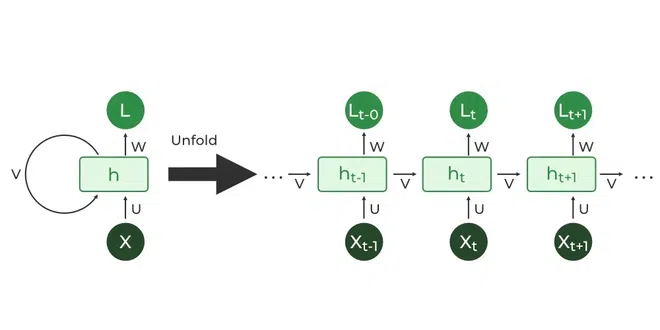
\includegraphics[width=0.55\textwidth]{rnn_image.png}
    \caption{Illustration du fonctionnement des Réseaux de Neurones Récurrents (RNN). Source : \url{https://miro.medium.com/v2/resize:fit:660/1*uLTBA8Myf6_IwtpfLr4Xpg.png}}
    \label{fig:rnn_architecture}
\end{figure}

\subsection{Long Short-Term Memory (LSTM)}

Les réseaux Long Short-Term Memory (\gls{lstm}) représentent une extension sophistiquée des réseaux de neurones récurrents (\gls{rnn}) traditionnels, conçue pour remédier à leurs limitations dans la capture des dépendances à long terme, notamment les problèmes de disparition ou d'explosion du gradient. Introduite par Hochreiter et Schmidhuber en 1997 \cite{hochreiter1997long}, l’architecture \gls{lstm} repose sur une cellule mémoire interne capable de conserver de l’information sur de longues séquences, contrôlée par un système de portes spécialisées.

À chaque instant temporel \( t \), les opérations fondamentales d'une cellule \gls{lstm} sont décrites par les équations suivantes :

\begin{align*}
f_t &= \sigma(W_f x_t + U_f h_{t-1} + b_f) \quad &\text{(Porte d'oubli)} \\
i_t &= \sigma(W_i x_t + U_i h_{t-1} + b_i) \quad &\text{(Porte d'entrée)} \\
\tilde{c}_t &= \tanh(W_c x_t + U_c h_{t-1} + b_c) \quad &\text{(État cellulaire candidat)} \\
c_t &= f_t \odot c_{t-1} + i_t \odot \tilde{c}_t \quad &\text{(Mise à jour de la cellule)} \\
o_t &= \sigma(W_o x_t + U_o h_{t-1} + b_o) \quad &\text{(Porte de sortie)} \\
h_t &= o_t \odot \tanh(c_t) \quad &\text{(État caché)}
\end{align*}

où :
\begin{itemize}
    \item \( x_t \) représente l’entrée à l’instant \( t \) ;
    \item \( h_{t-1} \) est l’état caché précédent ;
    \item \( f_t \), \( i_t \), \( o_t \) sont respectivement les vecteurs de la porte d’oubli, d’entrée et de sortie ;
    \item \( c_t \) désigne l’état de la cellule mémoire à l’instant \( t \) ;
    \item \( \tilde{c}_t \) est l’état cellulaire candidat proposé ;
    \item \( \sigma \) est la fonction sigmoïde, \( \tanh \) la tangente hyperbolique, et \( \odot \) désigne le produit élément par élément.
\end{itemize}

Cette structure permet aux \gls{lstm} de décider dynamiquement quelles informations conserver, mettre à jour ou émettre, offrant ainsi une capacité de mémorisation sélective très utile pour le traitement de séquences complexes. Grâce à cette flexibilité, les \gls{lstm} se sont imposés comme une référence dans de nombreuses tâches telles que la modélisation du langage, la traduction automatique, ou encore l’analyse de séries temporelles.

\begin{figure}[H]
    \centering
    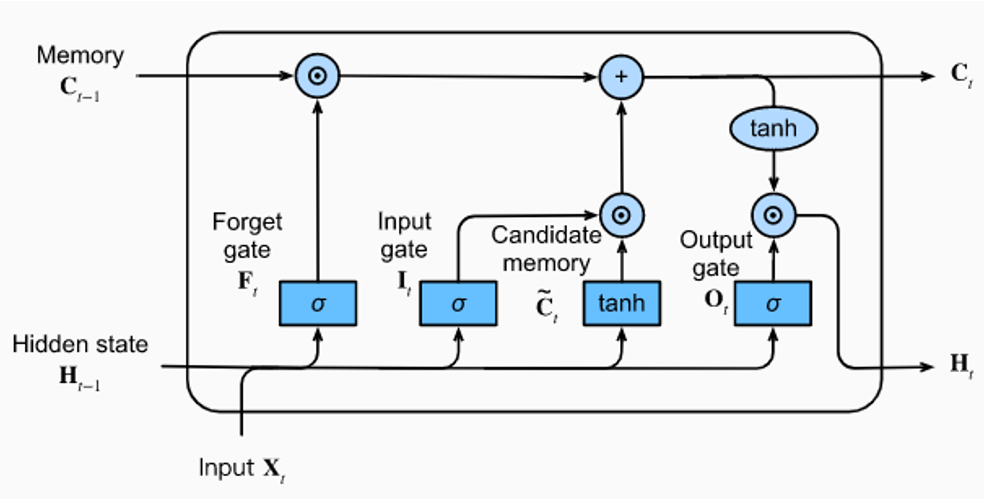
\includegraphics[width=0.55\textwidth]{lstm_image.png}
    \caption{Logique de l'architecture LSTM. Source : \url{https://sl.bing.net/bWWTQ1HkC7M}}
    \label{fig:lstm_architecture}
\end{figure}

\bigskip

\noindent Bien que puissants, les \gls{lstm} présentent une certaine complexité computationnelle en raison du nombre élevé de paramètres associés à leurs multiples portes. Pour proposer une alternative plus légère mais néanmoins efficace, la communauté a introduit une architecture simplifiée : le Gated Recurrent Unit (\gls{gru}).

\subsection{Gated Recurrent Unit (GRU)}

Le Gated Recurrent Unit (\gls{gru}) est une variante des \gls{rnn} introduite par Cho et al. en 2014 \cite{cho2014learning}, visant à réduire la complexité du modèle tout en maintenant des performances comparables à celles des \gls{lstm}. Contrairement aux \gls{lstm}, les \gls{gru} fusionnent les fonctions des portes d’oubli et d’entrée en une seule "porte de mise à jour", et n’utilisent pas d’état cellulaire distinct du vecteur caché. Cette simplification permet une convergence plus rapide et une efficacité accrue dans certaines tâches.

Les équations gouvernant une cellule \gls{gru} sont les suivantes :

\begin{align*}
z_t &= \sigma(W_z x_t + U_z h_{t-1} + b_z) \quad &\text{(Porte de mise à jour)} \\
r_t &= \sigma(W_r x_t + U_r h_{t-1} + b_r) \quad &\text{(Porte de réinitialisation)} \\
\tilde{h}_t &= \tanh(W_h x_t + U_h (r_t \odot h_{t-1}) + b_h) \quad &\text{(État candidat)} \\
h_t &= (1 - z_t) \odot h_{t-1} + z_t \odot \tilde{h}_t \quad &\text{(État caché)}
\end{align*}

où :
\begin{itemize}
    \item \( z_t \) est la porte de mise à jour ;
    \item \( r_t \) est la porte de réinitialisation ;
    \item \( \tilde{h}_t \) est l’état caché candidat ;
    \item \( h_t \) est l’état caché final de la cellule \gls{gru} à l’instant \( t \).
\end{itemize}

Cette architecture compacte permet aux \gls{gru} de s’adapter efficacement aux dépendances temporelles tout en limitant la charge computationnelle.

\begin{figure}[H]
    \centering
    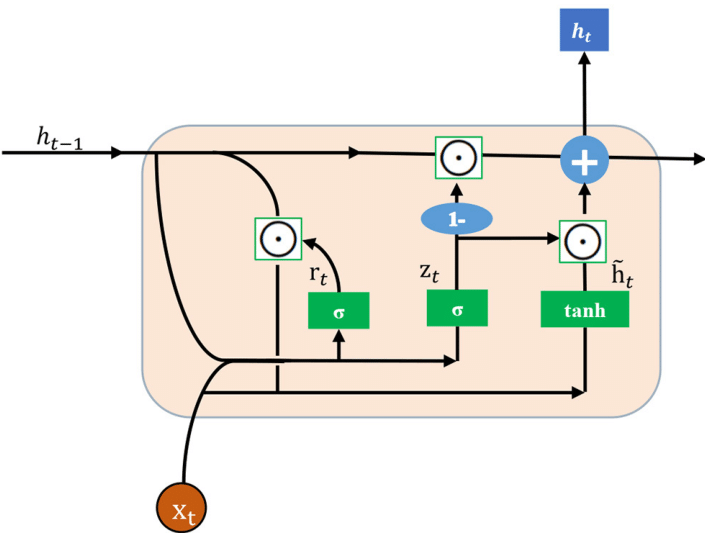
\includegraphics[width=0.45\textwidth]{gru_image.png}
    \caption{Illustration de l'unité récurrente à portes (GRU). Source : \url{https://sl.bing.net/bWWTQ1HkC7M}}
    \label{fig:gru_architecture}
\end{figure}

Cette architecture compacte permet aux \gls{gru} de s’adapter efficacement aux dépendances temporelles tout en limitant la charge computationnelle.

\vspace{0.5cm}

Cependant, malgré leur capacité à capturer des relations à long terme, les architectures séquentielles comme les \gls{lstm} et les \gls{gru} traitent les séquences de manière uniforme, sans accorder plus d’importance à certaines parties du texte qu’à d’autres. Pour pallier cette limitation, des mécanismes d’attention ont été introduits afin de permettre au modèle de se concentrer dynamiquement sur les éléments les plus pertinents de la séquence.

Parmi ces approches, le mécanisme d’attention proposé par Bahdanau et al. \cite{bahdanau2015neural} s’est imposé comme une extension efficace, initialement conçue pour la traduction automatique. Dans le cadre de ce mémoire, une adaptation simplifiée de cette attention est utilisée pour pondérer les sorties d’un \gls{gru} bidirectionnel dans une tâche de classification. La section suivante détaille ce mécanisme.

\section{Réseaux de Neurones Convolutionnels (CNN)}

Les réseaux de neurones convolutionnels (\gls{cnn}) sont des architectures largement utilisées en vision par ordinateur, mais leur application au traitement automatique du langage naturel (\gls{tln}) s’est révélée tout aussi prometteuse, notamment dans des tâches de classification de textes \cite{kim2014convolutional}. Leur principe repose sur l’extraction hiérarchique de caractéristiques à l’aide de filtres convolutifs glissants appliqués à une matrice représentant une séquence textuelle. 

Mathématiquement, l’opération de convolution discrète appliquée à une matrice d’entrée \( I \) et un noyau \( K \) est définie comme suit :

\begin{equation}
S(i, j) = (I * K)(i, j) = \sum_m \sum_n I(i + m, j + n) \cdot K(m, n)
\end{equation}

où \( S(i,j) \) désigne la sortie convoluée à la position \( (i,j) \), et les indices \( m,n \) parcourent les dimensions du filtre. Cette opération permet de détecter localement des motifs pertinents dans la structure du texte représenté sous forme matricielle.

Dans le cas d’un document textuel, chaque mot est d’abord représenté par un vecteur dense — soit appris durant l’entraînement, soit préentraîné (par exemple via \gls{glove} ou \gls{fasttext}). Ces vecteurs sont empilés pour former une matrice d’entrée de taille $L \times d$, où $L$ est la longueur du texte (ou le nombre de mots), et $d$ la dimension de l’embedding. Cette matrice est ensuite soumise à une \textit{couche de convolution}: des filtres (ou noyaux) glissent sur les lignes de la matrice, capturant des motifs locaux (comme des n-grammes) d’une taille fixée — par exemple, des fenêtres de 2, 3 ou 4 mots. Chaque filtre apprend à détecter une structure particulière (co-occurrence de termes, expressions spécifiques, tournures syntaxiques, etc.).

À la suite de cette convolution, une \textit{fonction d’activation} non linéaire, telle que la fonction ReLU (\textit{Rectified Linear Unit}), est généralement appliquée. Elle permet d’introduire de la non-linéarité dans le modèle et favorise la détection de motifs complexes.

Vient ensuite une \textit{opération de pooling}, souvent un max-pooling, qui réduit la dimension des représentations tout en conservant les informations les plus saillantes. Cette opération permet de rendre le modèle invariant aux petites variations dans la position des motifs détectés. Dans le cadre du \gls{tln}, cela revient à identifier les motifs les plus informatifs, quelle que soit leur position dans le texte.

Les représentations extraites par les filtres sont ensuite concaténées puis transmises à une ou plusieurs couches entièrement connectées (\textit{fully connected layers}), menant à une couche de sortie, généralement une \textit{softmax} (dans le cas de classification multiclasse) ou une \textit{sigmoid} (dans le cas binaire).

\begin{align}
\textit{sigmoid :} \quad \sigma(x) &= \frac{1}{1 + e^{-x}} \\[1em]
\textit{softmax :} \quad \text{softmax}(z_i) &= \frac{e^{z_i}}{\sum_{j=1}^{K} e^{z_j}} \quad \text{pour } i = 1, \dots, K
\end{align}

L’un des avantages majeurs des \gls{cnn} dans le traitement du texte est leur capacité à extraire des représentations discriminantes sans dépendre d’une modélisation explicite de l’ordre global de la séquence, tout en étant plus rapides à entraîner que les réseaux récurrents. En revanche, ils peinent parfois à capturer des dépendances à longue portée, raison pour laquelle ils sont souvent combinés à des architectures comme les \gls{gru} ou \gls{lstm}, comme c’est le cas dans ce mémoire avec les modèles hybrides \gls{cnn}-\gls{gru} et \gls{cnn}-\gls{lstm} \cite{zhou2015clstm}.

Ces architectures combinées bénéficient à la fois de la capacité des \gls{cnn} à extraire rapidement des motifs locaux, et de la capacité des réseaux récurrents à modéliser la dynamique temporelle et contextuelle des séquences. Cela en fait des candidats particulièrement pertinents pour la classification de textes biomédicaux, où les documents sont courts, denses en information, et s’appuient sur des structures linguistiques spécialisées.

\subsection{Mécanisme d’attention de Bahdanau}

Le mécanisme d'attention de Bahdanau, introduit dans le contexte de la traduction automatique neuronale \cite{bahdanau2015neural}, vise à surmonter les limitations des modèles séquentiels classiques qui compressent toute l’information d’une séquence dans un vecteur fixe. Cette compression peut être sous-optimale, notamment lorsque les séquences sont longues ou contiennent des informations dispersées.

L’attention permet au modèle de pondérer dynamiquement les éléments de la séquence en fonction de leur pertinence pour la tâche à accomplir. Autrement dit, au lieu de traiter toutes les parties d’un texte de manière égale, le modèle apprend à se concentrer davantage sur certaines parties pertinentes pour la prédiction.

Dans ce mémoire, une version simplifiée du mécanisme de Bahdanau est appliquée sur les sorties d’un \gls{gru} bidirectionnel. Concrètement, chaque sortie temporelle du \gls{gru} est transformée via un réseau feedforward afin de produire une importance (ou score d’attention). Ces scores sont ensuite normalisés via une fonction softmax pour obtenir des poids d’attention. Le vecteur de contexte est alors calculé comme une moyenne pondérée des états cachés de la séquence, où les poids reflètent la pertinence de chaque mot.

Le vecteur caché à un instant \( t \) dans un \gls{gru} bidirectionnel est défini comme la concaténation des vecteurs issus de la direction avant et arrière de la séquence :

\[
h_t = [\overrightarrow{h_t}; \overleftarrow{h_t}]
\]

où \( \overrightarrow{h_t} \) et \( \overleftarrow{h_t} \) sont respectivement les états cachés générés par les passes avant et arrière du \gls{gru}.

Le score d'attention pour chaque état caché à l'instant \( t \) est calculé comme suit :

\[
\text{score}_t = \mathbf{v}^\top \tanh(\mathbf{W} [\overrightarrow{h_t}; \overleftarrow{h_t}])
\]

L'importance relative de chaque élément de la séquence est ensuite calculée par une fonction softmax :

\[
\alpha_t = \frac{\exp(\text{score}_t)}{\sum_{t'} \exp(\text{score}_{t'})}
\]

Enfin, le vecteur de contexte, qui résume l'information pertinente des états cachés de la séquence, est obtenu par une somme pondérée des états cachés :

\[
\text{context} = \sum_t \alpha_t [\overrightarrow{h_t}; \overleftarrow{h_t}]
\]

Dans ces équations :

\begin{itemize}
    \item \( h_t \) est le vecteur caché à l’instant \( t \), qui est la concaténation des états cachés des directions avant et arrière;
    \item \( \alpha_t \) est le poids d’attention associé à l’état caché \( h_t \);
    \item \( \text{context} \) est le vecteur résultant, qui résume la séquence en mettant l’accent sur les éléments les plus pertinents.
\end{itemize}

Ce mécanisme permet au modèle d'exploiter à la fois les informations contextuelles antérieures et postérieures dans une séquence, ce qui est particulièrement utile pour des tâches comme la classification de textes biomédicaux, où un terme peut avoir un sens différent selon le contexte avant ou après son apparition.
\newline

Après avoir exploré le mécanisme d'attention de Bahdanau et son application dans des modèles séquentiels comme le \gls{gru} bidirectionnel, il est important de se pencher sur une autre composante essentielle dans les architectures de traitement du langage naturel : la représentation des mots et des phrases sous forme vectorielle. Ces représentations jouent un rôle fondamental dans la capture des relations sémantiques et contextuelles entre les termes.

Dans cette optique, plusieurs techniques de représentation vectorielle ont émergé pour mieux comprendre et modéliser le langage. Parmi les plus populaires, on trouve \gls{glove}, \gls{fasttext}, ainsi que des modèles de plus grande envergure spécifiquement conçus pour les domaines biomédicaux, tels que \gls{pubmedbert} et \gls{biobert}. Ces approches ont permis de dépasser les limites des représentations classiques, en intégrant à la fois des informations globales (comme les cooccurrences de mots) et des informations contextuelles plus fines.

La section suivante présente ces différentes techniques de représentation vectorielle, en mettant particulièrement l'accent sur leur application dans le domaine biomédical, où les termes sont souvent hautement spécialisés et contextuellement dépendants.

\vspace{0.5cm}
\section{Représentations de Vecteurs }

Les performances des modèles de traitement du langage naturel dépendent en grande partie de la manière dont les mots sont représentés numériquement. En effet, avant même l'application de modèles séquentiels ou de mécanismes d’attention, les textes doivent être transformés en vecteurs exploitables par les algorithmes d'apprentissage automatique.

Deux grandes familles de représentations vectorielles se distinguent : les \textit{word embeddings} statiques, qui attribuent un vecteur fixe à chaque mot indépendamment de son contexte, et les \textit{contextual embeddings}, qui ajustent dynamiquement les représentations en fonction du contexte d’apparition du mot dans la phrase.

Dans cette section, nous explorons tout d’abord les approches classiques basées sur les \textit{word embeddings}, notamment \gls{glove} et \gls{fasttext}, qui ont marqué une avancée significative dans la capture des relations sémantiques entre les mots. Ensuite, nous présentons des méthodes plus récentes et plus puissantes reposant sur des modèles de type Transformer, comme \gls{biobert} et \gls{pubmedbert}, qui produisent des représentations contextuelles particulièrement adaptées aux textes biomédicaux.

\subsection{Word Embeddings: GloVe and FastText}

Les \textit{word embeddings} statiques permettent de représenter chaque mot par un vecteur dense dans un espace continu de dimension réduite. Ces représentations sont apprises à partir de grands corpus de textes en exploitant les cooccurrences entre les mots. Deux des approches les plus influentes dans ce domaine sont \gls{glove} et \gls{fasttext}.

\begin{figure}[H]
    \centering
    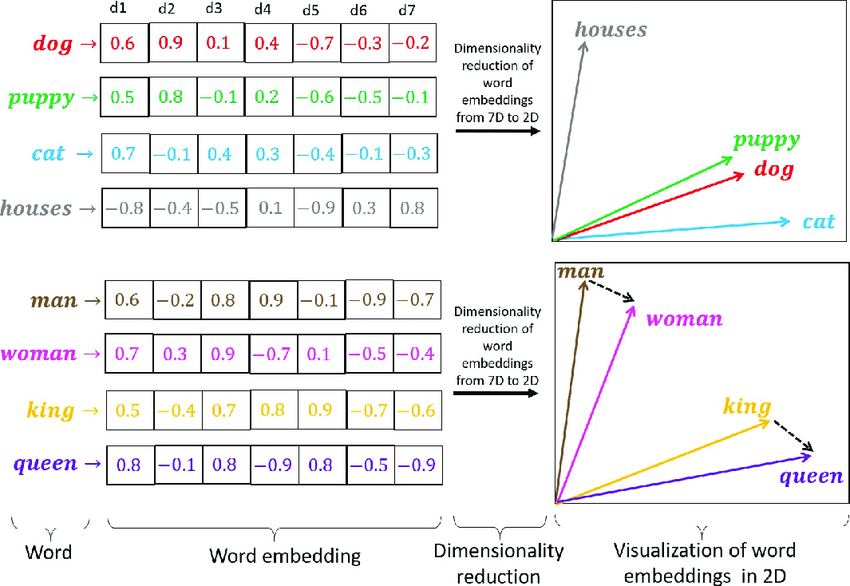
\includegraphics[width=0.65\textwidth]{we.png}
    \caption{Illustration du principe des \textit{word embeddings} : les mots similaires sont projetés dans des régions proches de l’espace vectoriel. Source : \url{https://sl.bing.net/jumSq5RbE1Q}}
    \label{fig:word_embeddings}
\end{figure}

\subsubsection{FastText}

\gls{fasttext} \cite{bojanowski2017enriching}, développé par Facebook \gls{ia} Research, est une extension de \gls{w2v}, une méthode d’apprentissage de représentations vectorielles des mots développée par Mikolov et al. Contrairement à \gls{glove} ou \gls{w2v}, qui considèrent chaque mot comme une unité atomique, \gls{fasttext}  représente un mot comme la somme des vecteurs de ses sous-unités, appelées \textit{n-grammes} de caractères. Formellement, si un mot \( w \) est composé de n-grammes \( g_1, g_2, \dots, g_K \), alors sa représentation vectorielle \( \mathbf{v}_w \) est définie comme :

\[
\mathbf{v}_w = \sum_{k=1}^{K} \mathbf{z}_{g_k}
\]

où \( \mathbf{z}_{g_k} \) est le vecteur associé au n-gramme \( g_k \).

Par exemple, le mot `chat'' avec des trigrammes (n=3), serait représenté par les n-grammes suivants : \_ch'', cha'', hat'', at\_''. \gls{fasttext} ajoute également des délimiteurs de mot (\_'' au début et à la fin) pour distinguer les positions dans le mot.

Cette représentation permet au modèle de partager l'information entre les mots ayant des morphologies similaires, ce qui le rend robuste aux mots rares ou inconnus (\textit{out-of-vocabulary}). De plus, FastText est capable de produire des vecteurs pour des mots absents du vocabulaire d’entraînement, tant que leurs sous-unités ont été observées.

En conservant les propriétés sémantiques de \gls{w2v} tout en capturant des régularités morphologiques (préfixes, suffixes, racines), FastText est particulièrement adapté à des domaines spécialisés comme le biomédical, où les termes sont souvent longs, composés et rares.

\subsubsection{GloVe}

\gls{glove} \cite{pennington2014glove} est une méthode d'apprentissage non supervisée qui combine les avantages des approches basées sur les fenêtres locales (comme \gls{w2v}) et des méthodes statistiques globales. Contrairement à Word2Vec, qui optimise une fonction de coût locale, \gls{glove} prend en compte des informations globales sur la distribution des mots dans le corpus entier. Il repose sur la construction d'une matrice de cooccurrence entre les mots dans un corpus, où chaque entrée \( X_{ij} \) correspond au nombre de fois que le mot \( j \) apparaît dans le contexte du mot \( i \), c'est-à-dire une mesure de la fréquence des cooccurrences entre les mots.

L’objectif du modèle est d’apprendre des vecteurs \( w_i \) et \( \tilde{w}_j \) pour chaque mot \( i \) et contexte \( j \) de sorte que leur produit scalaire approche le logarithme de \( X_{ij} \). Ce modèle s'exprime ainsi par la relation suivante :

\[
w_i^\top \tilde{w}_j + b_i + \tilde{b}_j \approx \log(X_{ij})
\]

où \( b_i \) et \( \tilde{b}_j \) sont des biais appris pour chaque mot et chaque contexte respectivement. Ce modèle est entraîné à optimiser cette relation sur toutes les paires de mots fréquents dans le corpus. L'optimisation de cette fonction permet de capturer les relations sémantiques et syntaxiques entre les mots. En particulier, les vecteurs appris par \gls{glove} sont capables de capturer des analogies de type :

\[
\vec{\text{roi}} - \vec{\text{homme}} + \vec{\text{femme}} \approx \vec{\text{reine}}
\]

Les embeddings produits par \gls{glove} sont ainsi capables de représenter des relations complexes entre les mots, non seulement sémantiques, mais aussi analogiques, ce qui les rend particulièrement utiles dans des applications de traitement du langage naturel comme la classification de texte, la recherche d'informations, et la génération de texte.

Un avantage clé de \gls{glove} est qu'il combine les informations locales de cooccurrence avec une représentation globale du corpus, ce qui permet d'apprendre des représentations de mots qui capturent non seulement des relations sémantiques proches mais aussi des relations plus abstraites, comme les analogies. Contrairement aux modèles locaux, qui se concentrent uniquement sur les relations entre les mots dans une fenêtre fixe, \gls{glove} intègre toute la structure globale des cooccurrences.

Cependant, une limitation de \gls{glove} réside dans son incapacité à gérer les ambiguïtés contextuelles des mots. Par exemple, le mot "banco" peut avoir des significations très différentes selon le contexte, mais \gls{glove} produira une seule représentation vectorielle qui ne tiendra pas compte de ces variations. Ce manque de contextualisation a motivé l'émergence de modèles plus avancés, tels que les modèles de représentation contextuelle des mots (par exemple, \gls{bert}), qui abordent ce problème en générant des embeddings différents en fonction du contexte dans lequel le mot apparaît.

\begin{figure}[H]
    \centering
    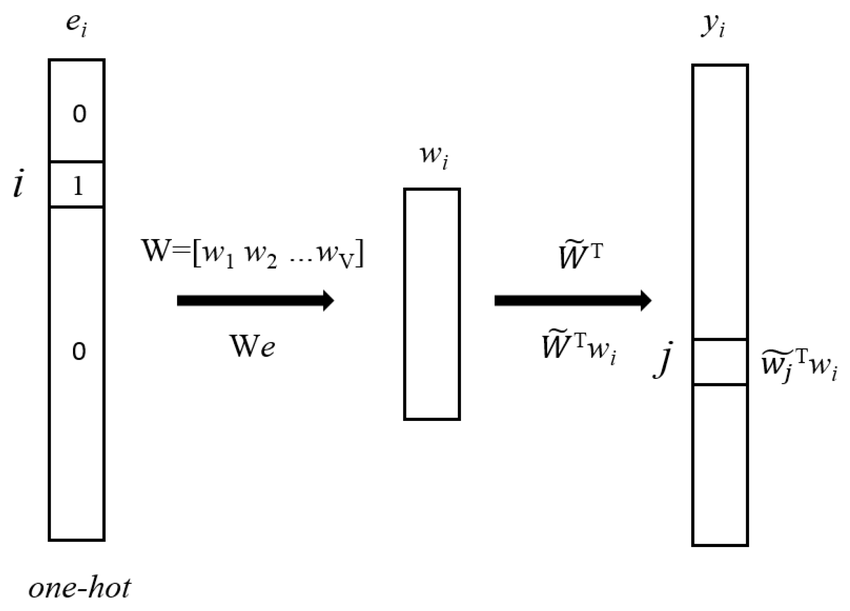
\includegraphics[width=0.35\textwidth]{glove.png}
    \caption{Architecture du modèle GloVe, illustrant la construction des vecteurs à partir des cooccurrences. L'entrée est une représentation \textit{one-hot} d’un mot à un instant donné. Les matrices d'intégration des mots sont utilisées comme matrices de poids, et la sortie du modèle est un vecteur obtenu par produit scalaire entre les vecteurs de mots. Source : \url{https://www.researchgate.net/figure/The-model-architecture-of-GloVe-The-input-is-a-one-hot-representation-of-a-word-The_fig1_337461648}}
    \label{fig:glove_architecture}
\end{figure}

% Ici, développe BioBERT et PubMedBERT
\subsection{Contextual Embeddings: BioBERT and PubMedBERT}

Bien que les \textit{word embeddings} statiques comme \gls{glove} et \gls{fasttext} aient significativement amélioré la qualité des représentations lexicales, ils présentent une limitation majeure : chaque mot y est associé à un vecteur unique, quelle que soit sa signification dans le contexte. Cela pose problème pour les mots polysémiques ou ambigus, fréquents dans le langage naturel et particulièrement critiques en biomédecine.

Pour pallier cette limite, les modèles récents s'appuient sur des architectures de type Transformer, capables de produire des représentations contextuelles dynamiques. Dans ces modèles, un même mot peut être représenté par des vecteurs différents selon le contexte dans lequel il apparaît.

Dans cette section, nous explorons deux représentations contextuelles spécialement entraînées sur des corpus biomédicaux : \gls{biobert} et \gls{pubmedbert}. Ces modèles, basés sur l’architecture de \gls{bert}, capturent des nuances sémantiques essentielles pour des tâches complexes telles que l’extraction d’informations biomédicales, la classification de documents scientifiques, ou encore la normalisation de concepts médicaux.

\subsection{BioBERT comme vecteur de plongement contextuel}

\gls{biobert} est une variante du modèle \gls{bert} spécialement préentraînée sur des corpus biomédicaux, tels que PubMed Abstracts et PMC Full-text articles \cite{lee2020biobert}. À l’instar de BERT, il génère des \textit{plongements de mots contextuels} (\textit{contextual embeddings}) : chaque mot est représenté par un vecteur dense qui dépend non seulement du mot lui-même, mais aussi de son contexte environnant.

Contrairement aux méthodes de plongement statique comme \gls{glove} ou \gls{w2v}, qui assignent un seul vecteur à chaque mot indépendamment du contexte, \gls{biobert} est capable de moduler dynamiquement les représentations en fonction des autres tokens présents dans la même phrase. Cela est rendu possible grâce à son architecture fondée sur des couches de type Transformer exploitant le mécanisme d’auto-attention (\textit{self-attention}).

Le mécanisme de self-attention calcule les dépendances entre tous les tokens d’une séquence, permettant à chaque mot de se représenter en fonction des autres :

\begin{equation}
\textit{Attention}(Q, K, V) = \text{softmax} \left( \frac{QK^{T}}{\sqrt{d_k}} \right) V
\end{equation}

où $Q$, $K$ et $V$ sont respectivement les matrices de requêtes, de clés et de valeurs dérivées des représentations d’entrée, et $d_k$ est la dimension des vecteurs clés. Cette opération permet au modèle de pondérer les interactions entre chaque paire de mots, capturant ainsi efficacement les relations sémantiques et syntaxiques, même à longue distance.

Le processus débute par une tokenisation via WordPiece (figure.~\ref{fig:wordpiece}), qui découpe les mots en sous-unités, puis par un encodage positionnel et segmentaire. Les tokens sont ensuite traités par plusieurs couches de Transformer, où le mécanisme d’auto-attention calcule, pour chaque token, une représentation vectorielle tenant compte de tous les autres tokens de la séquence. La sortie de ces couches est une série de vecteurs contextuels riches, adaptés à des tâches spécifiques comme la classification, la reconnaissance d’entités biomédicales ou l’extraction de relations.

\begin{figure}[H]
    \centering
    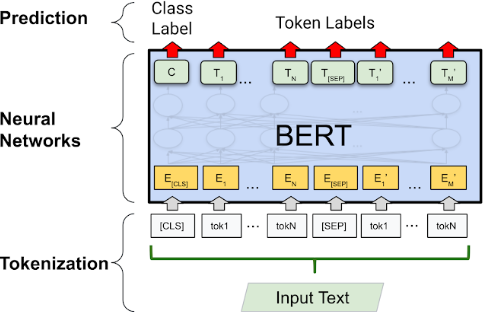
\includegraphics[width=0.5\textwidth]{tokenization_bert.png}
    \caption{Illustration du processus de tokenisation WordPiece suivi par l'encodage et les couches Transformer. Source : \url{https://research.googleblog.com/2021/12/a-fast-wordpiece-tokenization-system.html}}
    \label{fig:wordpiece}
\end{figure}

\gls{biobert} conserve l’architecture bidirectionnelle de \gls{bert} — chaque couche reçoit à la fois le contexte gauche et droit de chaque mot — mais il est initialisé avec les poids de \gls{bert} de base et affiné (\textit{fine-tuned}) sur de grands corpus biomédicaux. Cette spécialisation rend \gls{biobert} particulièrement performant dans les tâches du domaine de la santé : classification de textes biomédicaux, reconnaissance d'entités nommées, question-réponse clinique, etc.

\subsection{PubMedBERT comme vecteur de plongement contextuel}

\gls{pubmedbert} est une variante du modèle \gls{bert} qui a été préentraînée spécifiquement sur des textes biomédicaux extraits de la base de données PubMed, un des plus grands corpus de la littérature scientifique dans le domaine médical. PubMedBERT se distingue par le fait qu'il a été conçu pour mieux capturer les spécificités lexicales et les relations complexes qui existent dans les textes médicaux et biologiques, en particulier dans les domaines de la recherche biomédicale et des publications cliniques \cite{gu2020domain}. 

À l’instar de \gls{biobert}, \gls{pubmedbert} génère des \textit{plongements de mots contextuels} (\textit{contextual embeddings}) qui varient selon le contexte dans lequel les mots apparaissent. Cependant, \gls{pubmedbert} se distingue par son préentraînement exclusif sur les articles de PubMed, ce qui lui permet de mieux comprendre la terminologie et la sémantique propres à la biomédecine. En effet, \gls{pubmedbert} est capable de générer des vecteurs denses qui intègrent des informations spécifiques à la terminologie médicale, permettant ainsi des performances accrues dans des tâches comme l’extraction d’entités biomédicales, la classification de publications scientifiques ou encore l’analyse de relations entre concepts médicaux.

Le modèle s'appuie sur l’architecture Transformer et le mécanisme d’auto-attention pour produire des représentations vectorielles dépendant du contexte des mots, tout comme \gls{biobert}. La tokenisation initiale est réalisée à l’aide de WordPiece, un processus de découpage de mots en sous-unités qui permet une meilleure gestion des mots rares ou composés. Cela permet au modèle de traiter efficacement la grande variété de termes techniques rencontrés dans la littérature biomédicale.

Le processus de traitement des tokens dans \gls{pubmedbert} suit une approche similaire à celle de \gls{biobert} : une tokenisation via WordPiece (cf. Fig.~\ref{fig:wordpiece}) permet de découper les termes médicaux complexes en sous-unités, suivie par l'application d'un encodage positionnel et segmentaire. Les tokens sont ensuite passés par plusieurs couches de Transformer où chaque token est représenté par un vecteur contextuel calculé grâce au mécanisme d’auto-attention, prenant en compte l'ensemble des tokens de la séquence. La sortie de ces couches est une série de vecteurs contextuels qui sont utilisés pour des tâches spécifiques, telles que la classification de textes biomédicaux, l'extraction d'informations cliniques ou l'identification d'entités nommées dans des publications scientifiques.

Ainsi \gls{pubmedbert} est une solution puissante pour les applications biomédicales, où la compréhension fine de la terminologie médicale et scientifique est essentielle. Son préentraînement sur PubMed, combiné à l’architecture Transformer, lui permet d’obtenir de solides résultats dans des tâches complexes telles que la reconnaissance d'entités biomédicales, la classification de documents scientifiques et l’extraction d’informations cliniques, tout en prenant en compte les particularités linguistiques du domaine médical.

\section{Visualisation des représentations des données avec t-SNE}
\label{sec:tsne}

La visualisation des représentations vectorielles est une étape importante pour mieux comprendre comment un modèle de traitement du langage naturel apprend à distinguer les différentes classes à partir des données textuelles. Dans ce projet, nous utilisons l’algorithme \gls{tsne}~\cite{van2008visualizing} afin de projeter des vecteurs de haute dimension dans un espace bidimensionnel pour une visualisation intuitive.

\gls{tsne} (t-distributed Stochastic Neighbor Embedding) repose sur une modélisation probabiliste de la proximité entre points. Dans l’espace d’origine (de haute dimension), la similarité entre deux points $x_i$ et $x_j$ est définie comme une probabilité conditionnelle $p_{j|i}$, donnée par :

\begin{equation}
p_{j|i} = \frac{\exp(-\|x_i - x_j\|^2 / 2\sigma_i^2)}{\sum_{k \neq i} \exp(-\|x_i - x_k\|^2 / 2\sigma_i^2)}
\end{equation}

La probabilité symétrique conjointe est ensuite définie par :

\begin{equation}
p_{ij} = \frac{p_{j|i} + p_{i|j}}{2n}
\end{equation}

où $n$ est le nombre total de points. Dans l’espace projeté de faible dimension, une distribution $q_{ij}$ est définie sur les points projetés $y_i$ et $y_j$ en utilisant une distribution de Student à une seule liberté (plus lourde en queue que la Gaussienne) :

\begin{equation}
q_{ij} = \frac{(1 + \|y_i - y_j\|^2)^{-1}}{\sum_{k \neq l} (1 + \|y_k - y_l\|^2)^{-1}}
\end{equation}

L’objectif de \gls{tsne} est alors de minimiser la divergence de Kullback-Leibler (KL) entre ces deux distributions de similarité :

\begin{equation}
\mathcal{L} = KL(P \| Q) = \sum_{i \neq j} p_{ij} \log \left( \frac{p_{ij}}{q_{ij}} \right)
\end{equation}

Cette minimisation est effectuée par descente de gradient, et permet de préserver les structures locales des données — les paires de points proches en haute dimension restant proches dans l’espace 2D projeté.

Appliqué à différentes étapes du pipeline, \gls{tsne} permet d’obtenir une représentation visuelle des données telles qu’elles sont perçues par le modèle — que ce soit à l’entrée (par exemple, les embeddings de type \gls{glove} ou \gls{biobert}) ou à travers les activations intermédiaires après passage dans les couches du modèle (\gls{lstm}, attention, etc.).

L’interprétation des projections \gls{tsne} repose sur la conservation de la structure locale des données. En d’autres termes, si deux points sont proches dans l’espace projeté, ils étaient probablement aussi proches dans l’espace original à haute dimension. Ainsi, une bonne séparation visuelle entre groupes (ou classes) dans la carte \gls{tsne} peut indiquer que le modèle a appris des représentations discriminantes. À l’inverse, un chevauchement important peut signaler que les classes sont peu séparables dans l’espace appris, ce qui peut se traduire par des erreurs de classification.

Dans le cadre de ce travail, \gls{tsne} nous a permis de visualiser les regroupements de données issus de différentes classes, d'identifier des zones de confusion potentielle entre classes, et d'observer l'évolution des représentations apprises par le modèle au cours de l'entraînement.

Cette visualisation n’est pas simplement illustrative : elle offre une lecture qualitative du comportement du modèle et peut orienter des choix méthodologiques, par exemple en suggérant l’introduction de techniques de rééquilibrage ou l’ajustement de l’architecture si les classes restent difficilement séparables.

\section{L'apprentissage par petites touches dans le cadre du TALN : définitions, méthodes et défis}

L'apprentissage par petites touches \gls{fsl} représente une approche où les modèles doivent apprendre efficacement à partir de seulement quelques exemples par classe, un scénario couramment rencontré dans des contextes où il est difficile d'obtenir une quantité suffisante de données annotées. Cette approche est particulièrement utile en \gls{tln}, où les jeux de données peuvent être rares ou difficiles à annoter manuellement, comme dans les applications spécifiques à des domaines tels que la biomédecine ou le droit.

\subsection{Définitions et Concepts}

L'apprentissage par petites touches repose sur l'idée qu'un modèle peut apprendre des tâches complexes en utilisant très peu d'exemples. Cette capacité est essentielle pour surmonter les limitations des méthodes traditionnelles qui nécessitent de grandes quantités de données annotées pour obtenir de bonnes performances. Dans ce cadre, un k-shot se réfère au nombre d'exemples utilisés par classe pour entraîner un modèle. Par exemple, dans le cadre d'un problème de 5-shot learning, le modèle est entraîné avec cinq exemples par classe.

L'un des concepts clés du \gls{fsl} est la capacité des modèles à généraliser à partir de peu d'exemples. Cela nécessite de fortes capacités d'abstraction et de transfert de connaissances acquises lors de pré-entraînements sur des jeux de données plus larges, comme le montrent les travaux sur les architectures basées sur \gls{bert} et ses variantes \cite{devlin2019bert, lee2020biobert, lu2020pubmedbert}.

\subsection{Méthodes et Techniques}

Les méthodes de \gls{fsl} en \gls{tln} incluent des approches telles que le meta-learning (apprentissage de l'apprentissage), qui permet aux modèles de se former rapidement sur de nouvelles tâches avec peu d'exemples. Des techniques comme Matching Networks \cite{vinyals2016matching}, Prototypical Networks \cite{snell2017prototypical} et MAML (Model-Agnostic Meta-Learning) \cite{finn2017model} sont couramment utilisées. Ces méthodes se basent sur des mécanismes permettant au modèle d'apprendre à partir de peu d'exemples, en optimisant la capacité à adapter rapidement le modèle à de nouvelles tâches.

Les Transformers comme \gls{bert} \cite{devlin2019bert} et ses dérivés, tels que \gls{biobert} \cite{lee2020biobert} ou \gls{pubmedbert} \cite{lu2020pubmedbert}, ont été particulièrement efficaces dans les tâches de \gls{fsl} en TAL, car ils sont capables de capturer des représentations contextuelles riches et adaptatives. Ces modèles sont souvent pré-entraînés sur de vastes corpus et sont ensuite adaptés (fine-tunés) pour des tâches spécifiques avec peu d'exemples.

\subsection{Défis de l'Apprentissage par Petites Touches}

L'un des défis majeurs de l'apprentissage par petites touches est la généralisation. Le modèle doit être capable de faire des prédictions fiables malgré le nombre limité d'exemples d'entraînement. Cette difficulté est accentuée dans des domaines spécifiques comme la biomédecine, où la richesse sémantique et la polysémie des termes rendent le modèle susceptible de faire des erreurs si le contexte n'est pas bien compris \cite{jin2019recurrent, zhang2020biowordvec}. Les techniques telles que l'entraînement multitâche et le transfert d'apprentissage peuvent aider à surmonter ces obstacles en tirant parti de l'information présente dans des tâches ou des domaines similaires.

Le contraste entre les classes dans un jeu de données de Few-Shot peut également être un défi. Les modèles doivent être capables de distinguer des exemples très similaires tout en étant robustes aux variations dans les données d'entrée. Des approches comme l'augmentation de données et des techniques de régularisation peuvent être utiles pour améliorer la robustesse des modèles en \gls{fsl}. 

\section{Problèmes de déséquilibre des classes et techniques d’adaptation}
\label{sec:class-imbalance}

Le déséquilibre des classes est un problème fréquent dans la classification de textes biomédicaux, où certaines classes sont surreprésentées tandis que d’autres, souvent plus rares mais cliniquement importantes, sont sous-représentées. Cette disparité peut fortement biaiser l’apprentissage du modèle, qui tend alors à privilégier la classe majoritaire au détriment de la précision sur les classes minoritaires. Pour y remédier, plusieurs techniques d’adaptation ont été développées, parmi lesquelles des méthodes de rééchantillonnage et des stratégies de pondération des classes dans la fonction de perte. Ces techniques sont particulièrement pertinentes dans des contextes à faible volume de données ou à fort déséquilibre, comme en biomédecine.

\subsection{Méthodes de rééchantillonnage}

Les méthodes de rééchantillonnage visent à modifier la distribution des données afin de compenser le déséquilibre entre les classes. On distingue principalement deux approches :
\begin{itemize}
    \item le \textbf{suréchantillonnage}, qui augmente artificiellement la proportion des exemples minoritaires ;
    \item le \textbf{sous-échantillonnage}, qui réduit la taille des classes majoritaires pour équilibrer la distribution.
\end{itemize}

Bien que les deux types de méthodes soient couramment utilisés dans la littérature, notre projet se concentre exclusivement sur les techniques de \textbf{suréchantillonnage}. Ce choix repose sur une revue d’articles spécialisés dans l’apprentissage sur données déséquilibrées, notamment dans le domaine biomédical, où la conservation des données majoritaires est souvent cruciale pour préserver la richesse des cas cliniques. Par ailleurs, les méthodes de suréchantillonnage permettent d’enrichir la classe minoritaire sans altérer la structure globale du jeu de données.

Parmi les approches de suréchantillonnage, nous avons retenu deux techniques largement reconnues : \gls{smote} (Synthetic Minority Over-sampling Technique)~\cite{chawla2002smote} et sa variante Borderline-\gls{smote}~\cite{han2005borderline}. Ces méthodes ont démontré leur efficacité dans plusieurs études pour améliorer la performance des modèles sur des jeux de données fortement déséquilibrés.

\subsubsection{SMOTE — \textbf{Synthetic Minority Over-sampling Technique}}

\gls{smote}~\cite{chawla2002smote} est une méthode de suréchantillonnage qui vise à résoudre les problèmes de déséquilibre de classes dans les jeux de données, en particulier ceux où les classes minoritaires sont sous-représentées. Contrairement à des approches plus simples, comme la duplication aléatoire d’exemples minoritaires, \gls{smote} génère de nouveaux exemples synthétiques par interpolation, ce qui introduit une plus grande diversité dans les données.

Le principe fondamental de \gls{smote} consiste à sélectionner aléatoirement un des $k$ plus proches voisins d’un échantillon minoritaire, puis à créer un nouvel exemple le long du segment qui relie ces deux points dans l’espace des caractéristiques. Formellement, si $x_i$ est un exemple minoritaire et $x_i^{(NN)}$ l’un de ses voisins proches, un nouvel exemple synthétique $x_{\text{new}}$ est généré selon la formule :

\begin{equation}
x_{\text{new}} = x_i + \delta \cdot (x_i^{(NN)} - x_i), \quad \text{où } \delta \sim \mathcal{U}(0,1)
\end{equation}

où $\delta$ est un facteur de pondération aléatoire, tiré d’une distribution uniforme. Cette interpolation linéaire produit des instances qui sont proches des données existantes, tout en enrichissant l’espace des caractéristiques de la classe minoritaire de manière plus fluide que des duplications exactes.

Cette technique présente plusieurs avantages : elle réduit le risque de surapprentissage, améliore la définition des frontières de décision, et permet aux classifieurs d'apprendre à mieux généraliser dans les zones de faible densité. Elle est particulièrement pertinente dans les contextes biomédicaux où certaines conditions rares ou maladies spécifiques sont peu représentées dans les données.

Cependant, \gls{smote} présente également des limites. Notamment, il peut créer des instances synthétiques non représentatives si les voisins utilisés se trouvent près des frontières entre classes, ce qui peut introduire du bruit. De plus, en étendant artificiellement la minorité, il peut exacerber le chevauchement entre classes si le problème initial n'est pas linéairement séparable. Des variantes comme Borderline-\gls{smote} ont été proposées pour pallier ces inconvénients en adaptant la génération d’exemples aux zones les plus ambiguës.

Le principe de \gls{smote} est illustré dans la Figure~\ref{fig:smote_algo}, qui présente l'algorithme sous forme de pseudocode. Celui-ci détaille les étapes de génération d'exemples synthétiques par interpolation aléatoire entre un échantillon minoritaire et ses voisins les plus proches. Cette méthode peut être combinée à d’autres techniques, comme le sous-échantillonnage de la classe majoritaire ou la pondération de la fonction de perte, afin d’optimiser les performances sur des jeux de données déséquilibrés.

\begin{figure}[H]
    \centering
    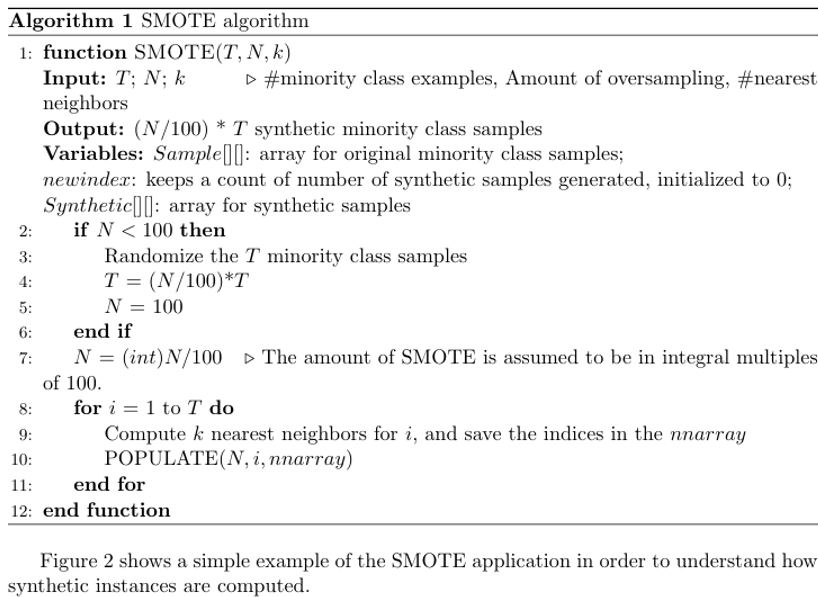
\includegraphics[width=0.8\textwidth]{smote.png}
    \caption{Algorithme \gls{smote} : génération d'exemples synthétiques à partir des voisins proches d'une instance minoritaire. Adapté de \cite{chawla2002smote}.}
    \label{fig:smote_algo}
\end{figure}

\subsubsection{Borderline-SMOTE}

Borderline-\gls{smote}~\cite{han2005borderline} est une variante de \gls{smote} qui cible spécifiquement les exemples situés à proximité des frontières de décision, c’est-à-dire les zones les plus susceptibles d’entraîner des erreurs de classification. Dans les applications sensibles comme le diagnostic médical, où les erreurs sur des cas ambigus peuvent être critiques, cette méthode renforce la capacité du modèle à discriminer correctement les classes dans les situations les plus complexes. Elle fonctionne en identifiant les échantillons minoritaires qui sont entourés de nombreux exemples de la classe majoritaire (situations "borderline") et en générant de nouveaux exemples à partir de ceux-là, afin de densifier ces zones critiques de l’espace de décision.

\section{Pondération des classes dans la fonction de perte}

La pondération des classes dans la fonction de perte est une méthode utilisée pour compenser le déséquilibre des classes en attribuant un poids plus élevé aux classes minoritaires. Cette approche permet de corriger le biais induit par un déséquilibre des classes sans altérer les données elles-mêmes. Elle est particulièrement utile dans les domaines où certaines classes sont cliniquement importantes mais sous-représentées, comme en biomédecine \cite{Chawla2002SMOTE} ou en science politique \cite{King2001Logit}.

Soit $y_i$ l'étiquette réelle de l'échantillon $i$, et $\hat{y}_i$ la prédiction du modèle pour cet échantillon. La fonction de perte classique pour une classification binaire (par exemple, l'entropie croisée) est donnée par :

$$
\mathcal{L}_\text{classique} = - \sum_{i=1}^{N} \left[ y_i \log(\hat{y}_i) + (1 - y_i) \log(1 - \hat{y}_i) \right]
$$

Cependant, dans le cas de classes déséquilibrées, cette fonction de perte peut entraîner un modèle qui favorise la classe majoritaire. Pour résoudre ce problème, on modifie cette fonction de perte en attribuant des poids $w_1$ et $w_0$ aux classes 1 et 0, respectivement. La fonction de perte pondérée devient alors :

$$
\mathcal{L}_\text{pondérée} = - \sum_{i=1}^{N} \left[ w_1 \cdot y_i \log(\hat{y}_i) + w_0 \cdot (1 - y_i) \log(1 - \hat{y}_i) \right]
$$

où $w_1$ et $w_0$ sont les poids associés respectivement aux classes 1 et 0. Ces poids peuvent être définis en fonction de la fréquence des classes dans le jeu de données. 


\vspace{1em}
Dans un problème multi-classe, chaque étiquette $y_i$ appartient à l'une des classes possibles, disons $C = \{1, 2, \dots, K\}$, où $K$ est le nombre total de classes. Le modèle prédit une probabilité $\hat{y}_i$ pour chaque classe $k$, c'est-à-dire $\hat{y}_i = P(\hat{y} = k | x_i)$ \cite{Han2005Borderline}.

La fonction de perte classique pour la classification multi-classe, telle que l'entropie croisée, est donnée par :

$$
\mathcal{L}_\text{classique} = - \sum_{i=1}^{N} \sum_{k=1}^{K} y_{ik} \log(\hat{y}_{ik})
$$

où $y_{ik}$ est l'étiquette binaire pour l'échantillon $i$ et la classe $k$ (soit 1 si $x_i$ appartient à la classe $k$, sinon 0), et $\hat{y}_{ik}$ est la probabilité prédite pour cette classe.

Pour adapter la fonction de perte au déséquilibre des classes dans un cadre multi-classe, on attribue un poids $w_k$ à chaque classe $k$. La fonction de perte pondérée devient alors :

$$
\mathcal{L}_\text{pondérée} = - \sum_{i=1}^{N} \sum_{k=1}^{K} w_k \cdot y_{ik} \log(\hat{y}_{ik})
$$

où $w_k$ est le poids associé à la classe $k$.

Comme pour le cas binaire, ces poids peuvent être définis de manière inversement proportionnelle à la fréquence des classes dans le jeu de données. Les poids peuvent être calculés de différentes manières, en fonction du déséquilibre des classes. 

La perte focale, proposée par Lin et al. \cite{Lin2017Focal}, cette méthode introduit un facteur de modulation pour focaliser l'apprentissage sur les exemples difficiles à classer, tout en conservant une pondération selon la classe (où $\gamma$ est un paramètre de focalisation) :
$$
\mathcal{L}_\text{local} = - \sum_{i=1}^{N} \sum_{k=1}^{K} w_k \cdot (1 - \hat{y}_{ik})^\gamma \cdot y_{ik} \log(\hat{y}_{ik})
$$.

\chapter{État de l’art}

\section{Panorama des méthodes de classification des textes biomédicaux}

La classification automatique de textes biomédicaux constitue un domaine central du traitement automatique du langage naturel (\gls{tln}), particulièrement essentiel pour des applications comme l'analyse des publications scientifiques, l'extraction d'informations cliniques ou encore les systèmes de soutien au diagnostic. Ce domaine a évolué parallèlement aux progrès réalisés en apprentissage automatique, et en particulier en apprentissage profond. L'objectif de cette section est de présenter l'évolution des approches de classification des textes biomédicaux, en se concentrant sur les travaux majeurs qui ont influencé ce domaine, tout en soulignant les motivations qui ont conduit à la réalisation de ce travail de thèse.

Dans les premières années de développement de la classification automatique des textes, les modèles étaient principalement basés sur des représentations simples comme le \textit{bag-of-words}. Ces approches traditionnelles incluaient également des méthodes comme les machines à vecteurs de support (SVM) ou encore les classifieurs Naïve Bayes. Ces techniques, bien que solides, peinaient à capturer les relations contextuelles complexes entre les termes, essentielles dans le domaine biomédical. Les corpus biomédicaux, souvent caractérisés par une forte spécialisation du vocabulaire et une grande ambiguïté sémantique, nécessitaient une approche plus sophistiquée, capable de comprendre ces relations subtiles.

L’évolution vers des modèles séquentiels a commencé dans les années 2010 avec l'émergence des réseaux neuronaux récurrents (\gls{rnn}), et plus particulièrement les variantes \gls{lstm} et \gls{gru}. Ces modèles ont permis de mieux modéliser les dépendances temporelles et contextuelles des mots dans une séquence de texte. En effet, dans des domaines comme la biologie ou la médecine, les relations entre les mots ne sont pas indépendantes, mais dépendent du contexte dans lequel ils apparaissent. Les \gls{rnn}, introduits par Elman (1990)~\cite{elman1990finding}, ont été les premiers modèles capables de traiter des séquences de données en capturant ces dépendances, mais ils souffraient d'un problème majeur : le phénomène du \textit{vanishing gradient} qui rendait difficile l'apprentissage sur de longues séquences. C’est dans ce contexte que les \gls{lstm}, proposés par Hochreiter et Schmidhuber (1997)~\cite{hochreiter1997long}, ont vu le jour, en introduisant des mécanismes de mémoire qui ont grandement amélioré la gestion de ces longues dépendances dans les données.

Les \gls{gru}, introduits plus récemment par Cho et al. (2014)~\cite{cho2014learning}, ont simplifié l'architecture des \gls{lstm}, tout en conservant des performances similaires, avec l'avantage de nécessiter moins de paramètres. Ces avancées ont permis une meilleure gestion des dépendances contextuelles, et ont donc trouvé une application naturelle dans le domaine biomédical, où il est crucial de capturer les relations entre les différentes entités médicales présentes dans un texte.

Parallèlement, les représentations de mots statiques comme \gls{w2v} et \gls{glove}, ainsi que des embeddings spécifiques au domaine comme BioWordVec~\cite{zhang2020biowordvec}, ont permis d’améliorer la représentation sémantique des termes. Ces modèles ont aidé à surmonter la limitation des représentations basées uniquement sur le comptage de mots, en fournissant des vecteurs denses qui capturent les relations sémantiques entre les mots.

Cependant, c'est avec l'essor des modèles basés sur les Transformers que la classification des textes biomédicaux a connu un véritable tournant. Les modèles tels que \gls{biobert}~\cite{lee2020biobert} et \gls{pubmedbert}~\cite{gupta2021pubmedbert}, préentraînés sur des corpus biomédicaux spécifiques, ont permis de capturer des relations contextuelles beaucoup plus fines, en prenant en compte l’ensemble du contexte autour d’un terme. Ces modèles ont permis de réaliser des avancées significatives dans la classification des textes médicaux, en particulier dans des tâches complexes comme l'extraction d'entités médicales et la reconnaissance de relations entre différentes entités.

À partir de 2018, la recherche s’est également orientée vers des scénarios plus complexes comme l’apprentissage par faible supervision (\gls{fsl}), où les modèles sont capables de s'adapter à des ensembles de données peu annotées ou déséquilibrées. Des techniques d'adaptation de domaine et de méta-apprentissage ont également été explorées pour permettre une meilleure généralisation et une plus grande robustesse des modèles face à des variations de langage ou des domaines spécifiques.

En nous appuyant sur ces différentes avancées, notre travail s'inscrit dans cette continuité de la recherche. Nous proposons de combiner ces techniques de manière innovante pour surmonter les défis spécifiques de la classification des textes biomédicaux, notamment la gestion du vocabulaire spécialisé, l'ambiguïté des termes et le déséquilibre des classes dans les corpus. Ce travail s’inspire largement des modèles séquentiels, en particulier des \gls{lstm}, \gls{gru} et des architectures récentes comme \gls{biobert}, pour aborder la classification dans ce domaine avec des solutions adaptées et performantes.

\subsection{Approches classiques}

Avant l’émergence des réseaux neuronaux profonds, la classification de textes biomédicaux reposait principalement sur des méthodes d’apprentissage automatique traditionnelles. Ces dernières s’appuyaient sur des représentations vectorielles creuses (\textit{sparse}), telles que le modèle \textit{Bag-of-Words} ou la pondération TF-IDF (\textit{Term Frequency–Inverse Document Frequency}), qui ignorent totalement l’ordre des mots ainsi que leur structure syntaxique ou sémantique. Les modèles classiques comme le classifieur Naïve Bayes, les machines à vecteurs de support (SVM) ou encore les arbres de décision étaient fréquemment utilisés, recevant en entrée ces vecteurs issus de représentations lexicales simples.

Par exemple, Japkowicz et Stephen (2002) \cite{japkowicz2002class} ont mis en évidence les limites de ces approches dans les contextes de déséquilibre des classes, phénomène courant dans les données biomédicales. De même, King et Zeng (2001) \cite{King2001Logit} ont étudié les performances dégradées des modèles de régression logistique face aux événements rares, ce qui pose un défi dans la classification de documents médicaux peu représentés. Si ces méthodes présentent l’avantage d’être interprétables et rapides à entraîner, elles ne permettent pas de capturer les relations sémantiques entre mots ni leur contexte d’apparition dans la phrase.

Ainsi, les modèles de classification de textes biomédicaux ont considérablement évolué avec les progrès du traitement du langage naturel et de l'apprentissage profond. Nous allons dans la suite nous concentrer sur les travaux spécifiques qui ont influencé la manière dont les modèles actuels sont utilisés dans le domaine biomédical. Dans les sections suivantes, nous explorerons des études précises, notamment celles portant sur l’application des \gls{lstm}, \gls{rnn} et des architectures plus complexes, pour mieux comprendre leurs contributions à la classification des textes dans le contexte biomédical. Ces travaux, tirés de la littérature, serviront de base à la conception et à l'implémentation de la méthode proposée dans ce travail de thèse.

Nous commencerons par examiner en détail les recherches ayant intégré des architectures récurrentes pour traiter des données biomédicales spécifiques, avant de nous intéresser aux récentes approches hybrides qui combinent plusieurs types de réseaux pour maximiser les performances de classification. Ces perspectives ouvriront la voie à la présentation de la méthodologie spécifique développée dans ce travail.

\subsection{Finding Structure in Time}

L’article fondateur de Jeffrey L. Elman intitulé \textit{Finding Structure in Time}~\cite{elman1990finding} marque une étape décisive dans l’évolution des modèles séquentiels pour le traitement du langage naturel. Dans ce travail, Elman introduit une architecture de réseau neuronal récurrent simple (SRN, \textit{Simple Recurrent Network}) destinée à apprendre des régularités temporelles dans des séquences linguistiques. Il ne s’agit pas simplement d’un développement technique, mais d’une démonstration empirique que des structures grammaticales et lexicales implicites peuvent émerger de l’exposition à des données séquentielles non annotées.

Le SRN fonctionne selon un principe fondamental : à chaque pas de temps $t$, l’entrée $x_t$ est combinée à un état de contexte $h_{t-1}$ (provenant de la couche cachée à l’instant précédent) pour produire un nouvel état caché $h_t$. Formellement, cela peut être représenté par :

\begin{equation}
h_t = \sigma(W_{xh} x_t + W_{hh} h_{t-1} + b_h), \quad y_t = \text{softmax}(W_{hy} h_t + b_y)
\end{equation}

où $\sigma$ est une fonction d’activation non linéaire (comme $\tanh$), $W_{xh}$, $W_{hh}$, et $W_{hy}$ sont des matrices de poids, et $y_t$ est la prédiction effectuée à l’instant $t$. La capacité du réseau à conserver l’information temporelle repose uniquement sur le passage récurrent de l’état caché, ce qui introduit une forme de mémoire.

Elman teste son modèle sur des tâches croissantes de complexité, démontrant que même un réseau récurrent simple peut développer des représentations internes qui capturent des structures linguistiques profondes :

\paragraph{Structure dans les séquences de lettres.} Le SRN est d’abord entraîné sur des séquences de lettres générées selon des règles probabilistes simples. Rapidement, le réseau parvient à prédire les lettres suivantes avec une précision significative, montrant qu’il a appris des régularités orthographiques implicites. Ce résultat suggère que l’apprentissage prédictif peut conduire à l’émergence de motifs structurés dans des flux continus de symboles.

\paragraph{Découverte implicite de la notion de mot.} Une expérience emblématique de l’article consiste à soumettre le SRN à un flux continu de caractères sans séparation explicite entre les mots. De façon remarquable, le réseau identifie implicitement les frontières lexicales, en capturant des statistiques de transition entre les lettres. Cette capacité d’induction structurelle sans supervision préfigure les modèles modernes d’apprentissage non supervisé.

\paragraph{Identification de classes lexicales à partir de l’ordre des mots.} Dans une tâche plus complexe, Elman expose le réseau à des séquences de mots respectant une grammaire artificielle. Le SRN apprend non seulement à prédire les éléments suivants mais organise les représentations internes de manière à regrouper les mots selon leur rôle grammatical (noms, verbes, déterminants, etc.). Ainsi, les représentations latentes révèlent l’acquisition spontanée de catégories syntaxiques.

Ce travail met en lumière plusieurs concepts clés : l’apprentissage distribué de représentations, l’importance de la mémoire dans le traitement séquentiel, et la capacité des réseaux à découvrir des structures hiérarchiques implicites. Il propose également des perspectives développementales : Elman postule que les contraintes temporelles et la capacité limitée de mémoire jouent un rôle dans la structuration progressive du langage chez l’enfant. Cette hypothèse a donné lieu à des travaux en psycholinguistique computationnelle, suggérant une convergence entre les processus d’apprentissage machine et cognitifs.

Cependant, le SRN souffre de limitations importantes, notamment le problème du gradient qui disparaît lors de la rétropropagation à travers le temps (\textit{vanishing gradient problem}), ce qui nuit à l’apprentissage de dépendances à long terme. Ces limites ont motivé l’émergence d’architectures plus robustes comme les réseaux LSTM~\cite{hochreiter1997long}, conçus spécifiquement pour surmonter ces difficultés.

En définitive, l’article de Elman constitue une pierre angulaire du développement des réseaux neuronaux pour le traitement du langage naturel, en montrant qu’un apprentissage prédictif simple peut induire une compréhension structurelle du langage. Ce paradigme reste central dans les architectures contemporaines, qu’il s’agisse des modèles récurrents, convolutionnels ou transformeurs.

\begin{figure}[H]
\centering
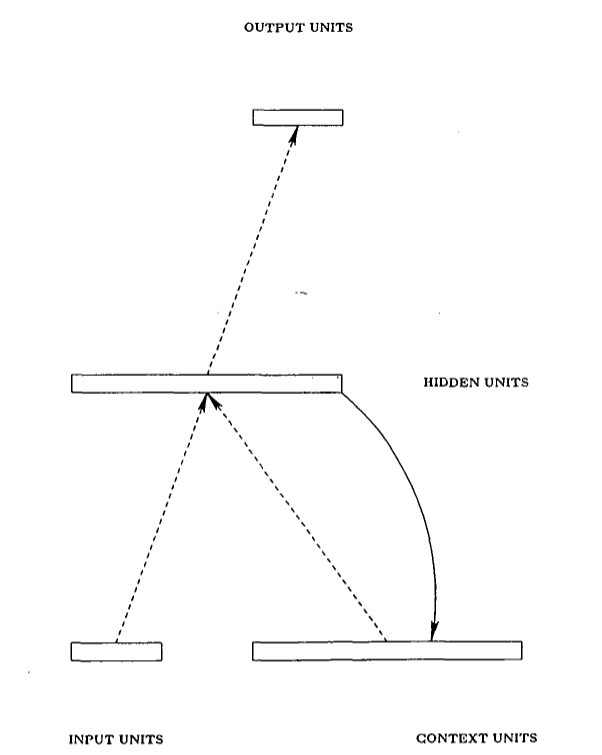
\includegraphics[width=0.3\linewidth]{rnn_elman.png}
\caption{Réseau récurrent simple selon Elman~\cite{elman1990finding}. Les activations de la couche cachée sont transférées à la couche de contexte avec un poids fixe de 1. Les connexions en pointillés sont les poids entraînables du réseau.}
\label{fig:elman_rnn}
\end{figure}

Enfin, l’article souligne que l’apprentissage efficace de structures hiérarchiques impose une contrainte sur la mémoire à court terme du réseau. Elman propose même une solution inspirée du développement humain : commencer l’apprentissage avec des séquences simples et augmenter progressivement leur complexité, une idée connue aujourd’hui sous le nom de \textit{curriculum learning}.

\subsection{Text Classification Improved by Integrating Bidirectional LSTM with Two-dimensional Max Pooling}

L’article de Zhou et al.~\cite{zhou2015text} propose une architecture innovante combinant un réseau bidirectionnel \gls{lstm} (BiLSTM) avec une opération de max pooling bidimensionnelle, dans le but explicite d'améliorer la classification des textes.

Le modèle repose d'abord sur un encodage bidirectionnel via un BiLSTM, qui permet de capturer simultanément les dépendances passées et futures dans une séquence. Contrairement aux \gls{rnn} classiques, le BiLSTM conserve des informations contextuelles des deux directions, ce qui est particulièrement utile dans le traitement des textes où les relations sémantiques peuvent dépendre de mots situés avant et après un terme cible.

Les auteurs utilisent des vecteurs de mots préentraînés \gls{glove}, construits à partir de 6 milliards de tokens issus de Wikipedia 2014 et du corpus Gigaword 5. Les mots absents de ce vocabulaire sont initialisés aléatoirement à l’aide d’une distribution uniforme dans l’intervalle $[-0{,}25, 0{,}25]$. Ces embeddings sont ensuite affinés pendant l’entraînement du modèle afin d’adapter les représentations lexicales à la tâche de classification.

L’innovation majeure introduite par les auteurs réside dans l’utilisation du \textit{2D max pooling} appliqué à la sortie du BiLSTM. Cette technique, inspirée des réseaux convolutionnels, permet d’extraire les caractéristiques les plus saillantes sur l’ensemble de la séquence encodée, réduisant ainsi le bruit et augmentant la robustesse du classifieur final. Grâce à cette combinaison, le modèle est capable de capturer non seulement des dépendances temporelles mais aussi des interactions locales plus fines entre les représentations cachées générées par le BiLSTM.

\begin{figure}[H]
    \centering
    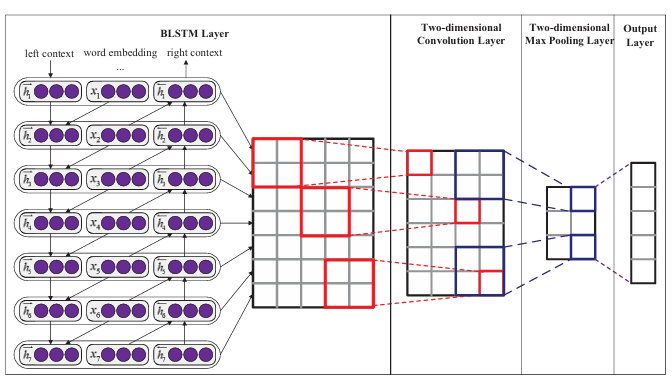
\includegraphics[width=0.5\textwidth]{bilstm.png}
    \caption{Architecture du modèle BLSTM-2DCNN pour une séquence de sept mots. Les vecteurs de mots ont une dimension de 3, et le BiLSTM comporte 5 unités cachées. La hauteur et la largeur des filtres convolutifs et des opérations de max pooling sont fixées à 2~\cite{zhou2015text}.}
    \label{fig:bilstm-arch}
\end{figure}

Les expérimentations, menées sur six jeux de données de classification textuelle (dont SST-1, SST-2, TREC, etc.), montrent que le modèle BLSTM-2DCNN surpasse non seulement les modèles \gls{rnn}, \gls{cnn} classiques, et les RecNN (Recursive Neural Networks), mais aussi les variantes proches comme le BLSTM-2DPooling ou le DSCNN (Deep Structured Convolutional Neural Network) proposé par Zhang et al.~(2016). Notamment, il atteint la meilleure précision sur les ensembles de données SST-1 et SST-2, souvent utilisés comme références dans les tâches de classification fine de sentiments.

Une analyse de sensibilité conduite sur SST-1 démontre également que l’utilisation de filtres convolutifs de grande taille permet de capturer davantage de motifs sémantiques complexes, ce qui peut améliorer significativement les performances. Ces résultats soulignent l’efficacité de la combinaison du BiLSTM avec des stratégies de réduction dimensionnelle en 2D, qui permettent de conserver à la fois les informations temporelles et les dimensions vectorielles issues des représentations de mots.

Ainsi, l’approche BLSTM-2DCNN représente une avancée notable dans la classification des textes, en offrant un compromis efficace entre richesse de représentation et simplicité de l’architecture, ce qui la rend particulièrement prometteuse pour des domaines complexes comme la biomédecine ou le juridique.

\subsection{BioBERT : Un modèle de langage préentraîné pour le domaine biomédical}

L’émergence des modèles de langage préentraînés comme \gls{bert} a révolutionné le traitement automatique du langage naturel (\gls{tln}), notamment en réduisant le besoin d’architectures spécifiques à chaque tâche grâce à un mécanisme d'attention bidirectionnelle. Cependant, malgré ses performances générales, \gls{bert} montre des limites dans les domaines spécialisés comme le biomédical, où le vocabulaire, la terminologie et les structures syntaxiques diffèrent notablement du langage général.

Pour répondre à cette problématique, Lee et al. (2020) ont introduit \gls{biobert}, une variante de \gls{bert} spécifiquement préentraînée sur de larges corpus biomédicaux, notamment les abstracts de PubMed (4,5 milliards de mots) et les articles en texte intégral de PMC (13,5 milliards de mots). L’objectif était d’adapter les représentations sémantiques de \gls{bert} au domaine biomédical, afin d'améliorer ses performances sur les tâches telles que la reconnaissance d’entités nommées (NER), l’extraction de relations (RE), et le question answering (QA).

\paragraph{Architecture de BioBERT.} \gls{biobert} reprend intégralement l'architecture de BERT\textsubscript{BASE}, composée de \textit{12 couches de transformeurs}, \textit{768 dimensions pour les représentations cachées}, \textit{12 têtes d’attention}, et environ \textit{110 millions de paramètres}. Il n’y a donc aucune modification structurelle par rapport à \gls{bert} ; l'amélioration provient uniquement du corpus de pré-entraînement et du vocabulaire spécialisé. \gls{biobert} est initialisé avec les poids de BERT\textsubscript{BASE} et continue le pré-entraînement avec un objectif de modélisation de langue masquée (MLM) sur les textes biomédicaux.

\begin{figure}[H]
    \centering
    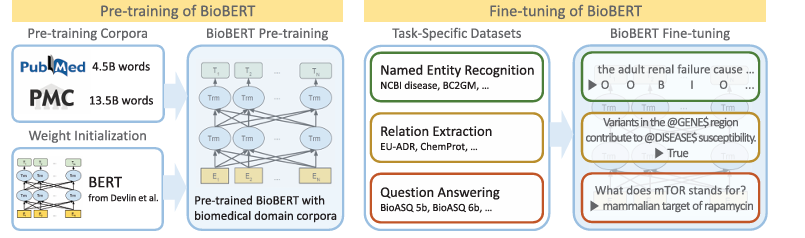
\includegraphics[width=0.75\textwidth]{biobert.png}
    \caption{Vue d'ensemble de la phase de pré-entraînement et de fine-tuning de BioBERT~\cite{lee2020biobert}.}
    \label{fig:biobert_architecture}
\end{figure}

Cette figure~\ref{fig:biobert_architecture} illustre le processus global de construction de \gls{biobert}, structuré en deux phases principales : le pré-entraînement et le fine-tuning. La première phase consiste à continuer l’entraînement du modèle BERT\textsubscript{BASE} sur de larges corpus spécialisés tels que PubMed et PMC, à l’aide de la tâche de modélisation de langage masqué (Masked Language Modeling). Cette étape vise à adapter les représentations linguistiques du modèle aux spécificités du domaine biomédical, sans modifier l’architecture initiale de \gls{bert}. La seconde phase, le fine-tuning, correspond à l’adaptation du modèle à des tâches précises du \gls{tln} biomédical telles que la reconnaissance d’entités nommées (NER), l’extraction de relations (RE) et le question answering (QA). Cette visualisation met en évidence que les gains de performance de \gls{biobert} ne proviennent pas d’un changement architectural, mais exclusivement du type et de la qualité du corpus utilisé lors de l’entraînement, soulignant ainsi l’importance des données spécialisées dans le succès de l’adaptation des modèles de langage préentraînés.

L'étude de Lee et al. (2020) a comparé différentes combinaisons de corpus pour le pré-entraînement, démontrant que plus le corpus est biomédical, meilleures sont les performances du modèle~\cite{lee2020biobert}:

\begin{table}[H]
\centering
\caption{Pré-entraînement de BioBERT selon les corpus textuels utilisés~\cite{lee2020biobert}}
\scriptsize
\resizebox{0.6\textwidth}{!}{%
\begin{tabular}{|l|l|}
\hline
\textbf{Modèle} & \textbf{Corpus utilisé} \\
\hline
BERT (baseline) & Wiki + Books \\
BioBERT (+PubMed) & Wiki + Books + PubMed \\
BioBERT (+PMC) & Wiki + Books + PMC \\
BioBERT (+PubMed + PMC) & Wiki + Books + PubMed + PMC \\
\hline
\end{tabular}%
}
\end{table}

L’évaluation de BioBERT a été menée sur plusieurs benchmarks de référence dans le domaine du traitement automatique du langage naturel biomédical. Ces benchmarks sont essentiels pour tester les capacités du modèle sur des tâches spécifiques et permettent de mesurer la performance de BioBERT sur des tâches fondamentales pour l’analyse et l’interprétation des textes biomédicaux. Parmi les principales tâches évaluées, on trouve la reconnaissance d’entités nommées (NER), l’extraction de relations (RE) et le question answering (QA).

La tâche de reconnaissance d’entités nommées, ou NER (Named Entity Recognition), consiste à identifier et classer les entités nommées présentes dans un texte. Ces entités peuvent inclure des termes comme les maladies, les médicaments, les gènes, etc. Plusieurs jeux de données ont été utilisés pour cette tâche, permettant de tester la capacité de BioBERT à reconnaître les entités médicales. Parmi ces jeux de données, on trouve le corpus NCBI Disease, qui contient des articles biomédicaux annotés sur les maladies, utilisé pour évaluer la capacité de BioBERT à identifier des entités médicales liées aux pathologies. Le jeu de données BC5CDR est spécifique à l’extraction d’entités liées aux maladies et aux médicaments, en mettant un accent particulier sur la relation entre les maladies et les substances chimiques. Le jeu JNLPBA, quant à lui, inclut des entités comme les protéines et les gènes, qui sont essentielles dans le domaine de la biologie moléculaire. Enfin, le corpus BioNLP13CG, provenant de la compétition BioNLP-2013, regroupe des entités relatives à la génomique, aux médicaments et à d’autres domaines de la biologie.

En ce qui concerne l’extraction de relations (RE), une autre tâche cruciale pour le traitement du langage biomédical, BioBERT a été évalué sur des jeux de données comme ChemProt et GAD. La tâche RE vise à identifier et classifier les relations entre différentes entités dans un texte, telles que les connexions entre maladies et traitements ou entre gènes et protéines. Le corpus ChemProt contient des relations entre substances chimiques et cibles biomoléculaires, et permet ainsi d’évaluer la capacité de BioBERT à extraire des relations biologiques. Le jeu de données GAD (Genetic Association Database), quant à lui, est utilisé pour détecter des relations entre des mutations génétiques et des maladies humaines, un domaine essentiel pour la génétique biomédicale.

Enfin, dans la tâche de question answering (QA), BioBERT a été testé sur le benchmark BioASQ, une compétition annuelle dédiée à l’extraction de réponses médicales à partir de PubMed et d'autres documents biomédicaux. Les questions posées dans BioASQ couvrent une large gamme de sujets médicaux et bioinformatiques, ce qui permet de tester la capacité de BioBERT à extraire des informations pertinentes et précises à partir de documents scientifiques complexes. Cette tâche est particulièrement importante dans un contexte où les médecins et chercheurs doivent pouvoir accéder rapidement à des réponses fiables basées sur une vaste quantité d’informations biomédicales.

\begin{figure}[H]
    \centering
    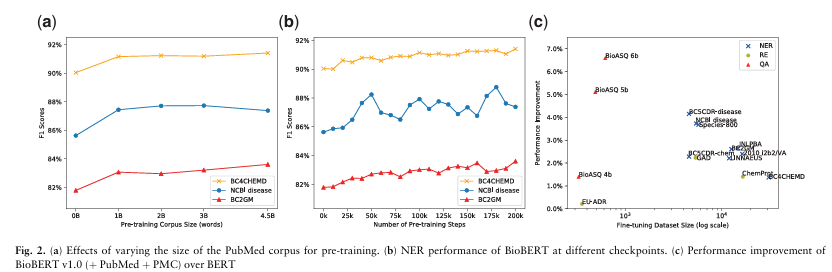
\includegraphics[width=0.8\textwidth]{result_biobert.png}
    \caption{(a) Effet de la taille du corpus PubMed sur le pré-entraînement. (b) Performances NER de BioBERT à différents checkpoints. (c) Amélioration obtenue par BioBERT v1.0 (PubMed + PMC) par rapport à BERT~\cite{lee2020biobert}.}
    \label{fig:biobert_results}
\end{figure}

Les auteurs de \gls{biobert} ont conduit une série d'expérimentations pour évaluer l'impact du volume de données biomédicales utilisées lors du pré-entraînement. Les résultats, illustrés dans la figure~\ref{fig:biobert_results}(a), montrent que l’augmentation progressive de la taille du corpus PubMed entraîne une amélioration significative des performances du modèle sur plusieurs tâches de reconnaissance d’entités nommées (NER). Plus précisément, les scores F1 augmentent de manière notable pour les jeux de données NCBI Disease, BC4CHEMD et BC5CDR. Toutefois, au-delà d’un certain seuil — environ 4,5 milliards de mots — les performances tendent à se stabiliser, indiquant que le modèle atteint une saturation en termes de bénéfices apportés par des données supplémentaires. Cela souligne qu’un pré-entraînement sur un large corpus biomédical est bénéfique, bien que l’effet marginal décroisse à mesure que le corpus s’élargit.

La figure~\ref{fig:biobert_results}(b) met en évidence l’évolution des performances de \gls{biobert} au cours du pré-entraînement, en fonction du nombre de pas d’apprentissage. On observe que les résultats s’améliorent globalement avec l’augmentation du nombre de pas, ce qui démontre la capacité du modèle à continuer à apprendre des représentations linguistiques pertinentes sur le long terme. Cette progression est particulièrement marquée pour certaines tâches comme celle du NCBI Disease, pour laquelle les fluctuations sont plus visibles mais tendent vers une convergence performante. Cette observation corrobore l'idée que le pré-entraînement prolongé, lorsqu’il est effectué sur un corpus spécialisé, permet une spécialisation fine du modèle aux subtilités du langage biomédical.

Enfin, la figure~\ref{fig:biobert_results}(c) compare directement les performances de \gls{biobert} par rapport au modèle \gls{bert} généraliste. L’amélioration est mesurée en fonction de la taille du jeu de données utilisé pour le fine-tuning, ce dernier étant représenté en échelle logarithmique. Il ressort de cette analyse que les gains les plus significatifs sont obtenus sur les tâches de question answering (QA), notamment sur les différentes versions de BioASQ, où l'amélioration dépasse les 6~\%. Les tâches de NER bénéficient également d’un gain notable, généralement compris entre 2~\% et 4~\%. En revanche, les tâches d’extraction de relations (RE) affichent des gains plus modestes, bien qu’ils restent constants. Un aspect particulièrement intéressant est que les plus fortes améliorations sont observées sur les jeux de données de petite taille, ce qui souligne l’intérêt de \gls{biobert} dans des contextes où les ressources annotées sont limitées. Ainsi, ces résultats confirment la pertinence du pré-entraînement sur des données spécialisées, et démontrent que la qualité du corpus joue un rôle central dans l’adaptation efficace des modèles de langage aux domaines spécifiques.

\newpage

\chapter{Architectures et expériences}

\section{Analyse exploratoire des données}

Les jeux de données analysés contiennent plusieurs variables textuelles ou métadonnées, décrites dans le tableau~\ref{tab:variables}. Parmi celles-ci, la variable \texttt{Abstract} a été retenue comme unique source d'information pour les tâches de classification. Elle contient un résumé riche et complet de l’article, intégrant la majorité des informations essentielles — y compris celles souvent redondantes avec les mots-clés ou les termes MeSH. Par conséquent, aucune procédure de sélection automatique de variables n’a été nécessaire. Ce choix permet de concentrer le traitement sur une seule séquence textuelle cohérente, tout en assurant une standardisation du pipeline de prétraitement.

Cette section propose une analyse exploratoire des deux jeux de données extraits de PubMed, contenant des résumés d’articles scientifiques liés à diverses pathologies. L’objectif est de mieux comprendre la structure des données, d’identifier des déséquilibres de classes, et de repérer certaines tendances textuelles pouvant influencer la performance des modèles.

Les deux jeux de données partagent les mêmes variables principales, notamment : un identifiant unique (\texttt{PMID}), le \texttt{Titre} de l’article, le \texttt{Résumé} (\texttt{Abstract}), les \texttt{Mots-clés}, l’année de publication (\texttt{PublicationYear}), les \texttt{MeSH Terms}, ainsi que l’étiquette de classe (\texttt{Label}). Une description complète de ces variables est disponible en annexe (voir Table~\ref{tab:variables}).

La première tâche concerne la classification binaire entre les articles liés au paludisme (classe 1) et ceux portant sur d’autres pathologies telles qu’Alzheimer ou la Dengue (classe 0). L’ensemble de données correspondant comporte \textit{29\,997} résumés (voir Figure~\ref{fig:word_distribution_binary_class}), collectés entre 1950 et 2024. La distribution des classes y est déséquilibrée, avec une surreprésentation des articles relatifs au paludisme. En termes de nombre de mots, le nombre de mots dans les résumés varie entre un minimum de 1 et un maximum de 4985 mots, avec une moyenne d’environ 243.86 mots par résumé.

La seconde tâche est une classification multiclasses impliquant \textit{42\,879} résumés, répartis en neuf catégories de maladies, allant de pathologies infectieuses (tuberculose, choléra, lèpre, etc.) à non infectieuses (leucémie, asthme, Parkinson, etc.) (voir Figure~\ref{fig:word_distribution_multi_class}). Ces données couvrent également la période de 1950 à 2024 et présentent un déséquilibre marqué entre les classes. Pour cette tâche, le nombre de mots dans les résumés varie de 0 (cellules vides) à 3814 mots, avec une moyenne de 219.25 mots par résumé.

À noter que les maladies infectieuses sont généralement causées par des agents pathogènes externes (bactéries, virus, parasites), tandis que les maladies non infectieuses résultent souvent de facteurs internes tels que des mécanismes chroniques, auto-immuns ou génétiques.

Les histogrammes des distributions des nombres de mots dans les résumés de ces deux tâches sont illustrés dans la Figure~\ref{fig:class_distributions}. Cette analyse permet de mieux comprendre les variations dans le nombre de mots, notamment les différences entre les résumés très courts et ceux plus détaillés, ce qui pourrait potentiellement influencer la performance des modèles de classification. Les histogrammes des distributions des mots pour chaque tâche sont présentés respectivement sous les Figures~\ref{fig:word_distribution_binary_class} et~\ref{fig:word_distribution_multi_class} en annexe.

\begin{center}
\begin{figure}[H]
\centering
\begin{minipage}{0.48\textwidth}
  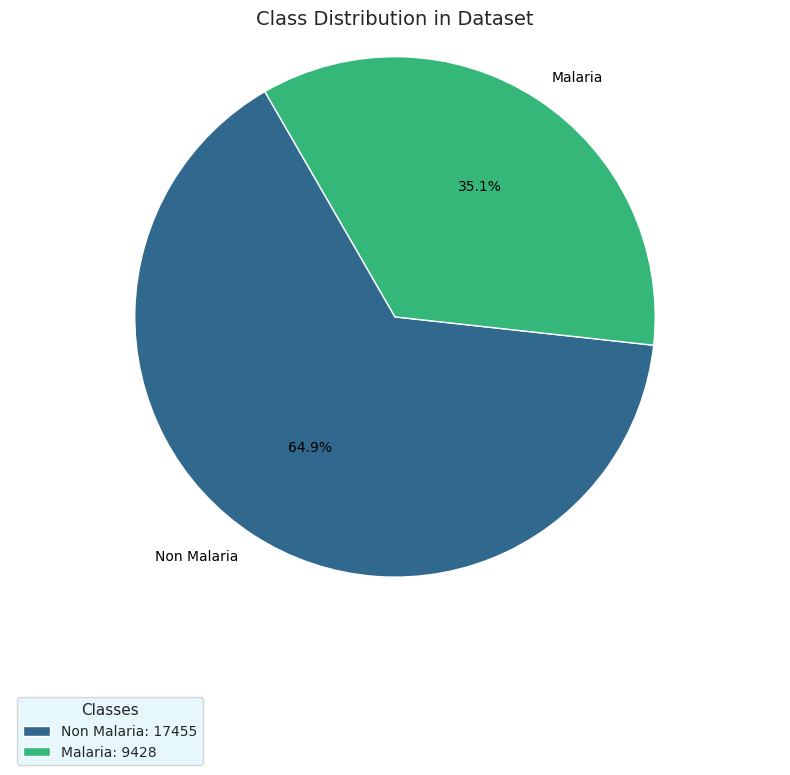
\includegraphics[width=0.65\linewidth]{binary_class_distribution.png}
\end{minipage}
\hfill
\begin{minipage}{0.48\textwidth}
  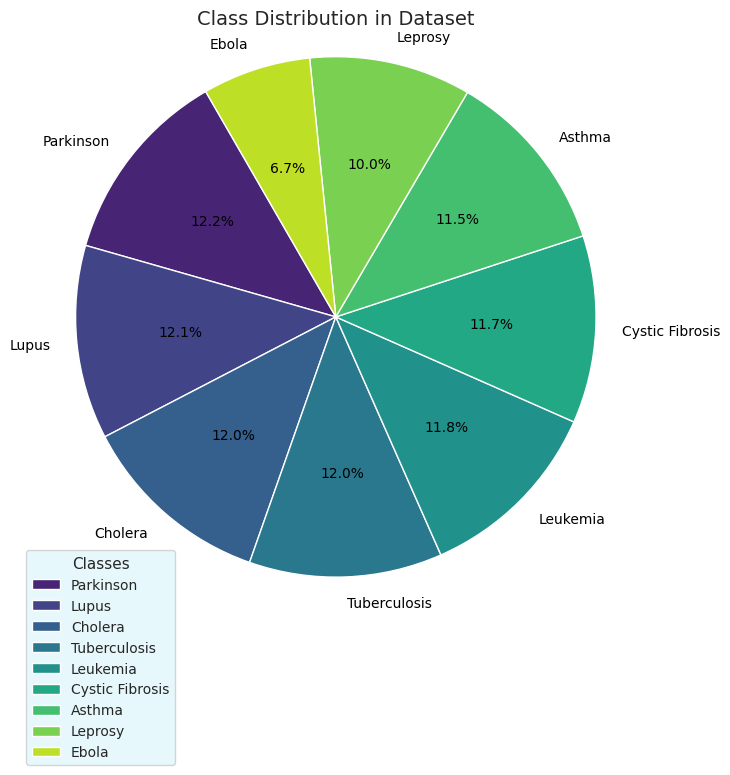
\includegraphics[width=0.65\linewidth]{multiclass_class_distribution.png}
\end{minipage}
\caption{Répartition des classes dans les jeux de données de classification binaire (gauche) et multiclasses (droite).}
\label{fig:class_distributions}
\end{figure}
\end{center}

\section{Prétraitement des données}

Le prétraitement des données est une étape clé dans la préparation des textes pour l’analyse. Il comprend plusieurs sous-étapes essentielles, notamment le nettoyage des textes, la tokenisation, la lemmatisation et la vectorisation.

Tout d'abord, les résumés sont nettoyés en supprimant les caractères spéciaux non pertinents, tout en conservant certains symboles mathématiques tels que les opérateurs de comparaison. Ensuite, le texte est converti en minuscules et les espaces inutiles sont éliminés pour standardiser les données.

Une fois le texte nettoyé, il est tokenisé, c'est-à-dire décomposé en mots individuels. À cette étape, la lemmatisation est appliquée. Chaque mot est réduit à sa forme de base (ou lemme), ce qui permet de minimiser la variabilité des termes tout en maintenant leur signification fondamentale. Par exemple, \textit{mangeraient}, \textit{mangeons} et \textit{manger} seraient tous réduits à \textit{manger}. De plus, les mots vides, c'est-à-dire les termes sans signification contextuelle importante (tels que \textit{et}, \textit{le}, \textit{de}), sont supprimés afin de ne conserver que les mots pertinents pour l'analyse.

Une fois les textes nettoyés et standardisés, le corpus est divisé en trois sous-ensembles distincts afin de structurer le processus d’entraînement. Le jeu de données est réparti en 70\% pour l’entraînement, 15\% pour la validation, et 15\% pour les tests. Cette séparation garantit une évaluation objective des modèles développés. L'ensemble d'entraînement est utilisé pour ajuster les paramètres du modèle, l'ensemble de validation permet de suivre la performance en cours d'entraînement et de détecter d’éventuels surapprentissages, tandis que l’ensemble de test fournit une estimation finale de la capacité du modèle à généraliser sur des données inédites.

Afin de mieux visualiser la répartition des termes dominants dans chaque tâche de classification, des nuages de mots ont été générés pour illustrer les termes les plus fréquents. Dans le nuage de mots pour la classification binaire, des termes comme \textit{parasite}, \textit{patient}, \textit{infection} et \textit{disease} ressortent en grande taille pour la classe 0, indiquant que ces termes sont particulièrement fréquents et significatifs dans les résumés relatifs à cette classe. En revanche, des mots tels que \textit{schistosomiasis}, \textit{prevalence}, et \textit{young} apparaissent en caractères plus petits, ce qui suggère qu’ils sont moins fréquents, mais toujours importants dans ce contexte.

Pour la classe 1, des mots comme \textit{malaria}, \textit{plasmodium}, et \textit{mosquito} sont affichés en grand, mettant en évidence leur importance et leur fréquence dans les résumés relatifs au paludisme. D'autres termes, tels que \textit{prevalence}, \textit{disease} et \textit{patient}, apparaissent en plus petites tailles, signifiant qu’ils sont également présents, mais dans une moindre mesure.

Un raisonnement similaire peut être appliqué à la classification multiclasses. Dans ce cas, les nuages de mots reflètent les caractéristiques uniques de chaque catégorie de maladie. Par exemple, pour les pathologies infectieuses, des termes comme \textit{tuberculosis}, \textit{cholera}, et \textit{leprosy} sont visibles en grand, tandis que pour les maladies non infectieuses, des mots comme \textit{leukemia}, \textit{asthma}, et \textit{Parkinson} dominent. Les termes généraux tels que \textit{disease}, \textit{prevalence}, et \textit{patient} sont présents dans les deux catégories, mais leur taille varie en fonction de leur fréquence dans les différentes classes.

Les résultats des nuages de mots pour chaque tâche de classification sont disponibles en annexe, respectivement dans les Figures~\ref{fig:binary_word_cloud} et~\ref{fig:multi_word_cloud}. Ces visualisations permettent de mieux comprendre la distribution des termes les plus significatifs dans les deux types de classification et offrent une perspective intéressante sur les caractéristiques sémantiques des données textuelles.

Dans le cadre des expériences impliquant des modèles entraînés sans embeddings préexistants (learn from scratch), ainsi que ceux utilisant des représentations vectorielles statiques telles que \gls{glove} et \gls{fasttext}, un pipeline spécifique de préparation des données a été développé. Ce pipeline inclut plusieurs étapes essentielles : la tokenisation des textes, la création d’un vocabulaire à partir du corpus d'entraînement, l'encodage des séquences en indices numériques, ainsi que le padding pour garantir une longueur uniforme des séquences. Un seuil de fréquence minimale est appliqué pour éliminer les mots rares, tandis que les termes absents du vocabulaire sont remplacés par un jeton spécial \texttt{<UNK>}. Les séquences sont ensuite converties en tenseurs, ce qui les rend compatibles avec l'entraînement de réseaux de neurones. Cette approche vise à fournir une représentation normalisée et cohérente du texte, particulièrement adaptée pour l’entraînement de modèles légers ou d’architectures récurrentes (\gls{lstm}/\gls{gru}), que ce soit avec des embeddings appris durant l’entraînement ou initialisés avec des matrices pré-entraînées comme celles de \gls{glove} ou \gls{fasttext}.

Lors des expériences impliquant des modèles utilisant des embeddings contextuels, un pipeline distinct est mis en place. Celui-ci repose sur l’utilisation d'un tokeniseur adapté, qui transforme chaque texte brut en une séquence de tokens, puis génère les identifiants d'entrée et les masques d'attention nécessaires. Le tokeniseur prend également en charge le padding et la troncature des séquences à une longueur maximale de 400 tokens, garantissant ainsi une taille uniforme des entrées. Ensuite, ces données sont intégrées dans une classe de dataset personnalisée, permettant de préparer les textes pour des modèles utilisant des embeddings contextuels. Les étiquettes de classification sont ajoutées sous forme de tenseurs, et chaque entrée est ainsi représentée par ses identifiants de tokens, ses masques d'attention et ses étiquettes correspondantes. 

\section{Présentation des architectures et types d’embeddings}

Afin de répondre aux deux tâches de classification (binaire et multiclasses), nous avons expérimenté plusieurs architectures de réseaux neuronaux, chacune combinée à des représentations textuelles différentes. Ces combinaisons visent à capturer des caractéristiques linguistiques et sémantiques variées, tout en tenant compte des contraintes de complexité et de temps de calcul.

Trois familles principales d’approches ont été explorées en termes de représentation des textes :

\begin{itemize}
    \item \textit{Sans embeddings pré-entraînés} : les vecteurs de mots sont appris \textit{from scratch} au cours de l'entraînement, ce qui peut convenir à des corpus très spécifiques mais exige généralement plus de données pour être efficace.
    
    \item \textit{Word embeddings statiques} : utilisation de vecteurs pré-entraînés tels que \texttt{GloVe} (300 dimensions) et \texttt{FastText} (300 dimensions). Ces représentations fournissent une sémantique enrichie mais restent fixes quel que soit le contexte d’apparition du mot.
    
    \item \textit{Embeddings contextuels} : recours à des modèles de type \gls{bert}, en particulier \gls{biobert} et \gls{pubmedbert}, spécifiquement entraînés sur des textes biomédicaux. Ces modèles produisent des représentations dynamiques, sensibles au contexte dans lequel chaque mot apparaît.
\end{itemize}

Concernant les architectures de modèles, les choix se sont appuyés sur des considérations à la fois théoriques (capacité de modélisation du langage), pratiques (temps d’inférence et d'entraînement), et empiriques (performances observées dans la littérature et sur des jeux similaires). Les combinaisons testées selon chaque tâche sont résumées ci-dessous :

\begin{itemize}
    \item \textbf{Tâche de classification binaire} :
    \begin{itemize}
        \item \gls{lstm} : capable de capturer des dépendances séquentielles à long terme.
        \item \gls{gru} : alternative plus efficace au \gls{lstm}, avec moins de paramètres à entraîner.
        \item \gls{gru} bidirectionnel avec attention de Bahdanau : mécanisme d’attention qui permet au modèle de se concentrer dynamiquement sur les segments pertinents du résumé, améliorant l’interprétabilité et la précision.
    \end{itemize}
    
    \item \textbf{Tâche de classification multiclasses} :
    \begin{itemize}
        \item \gls{lstm}, \gls{gru};
        \item \gls{cnn} + \gls{gru} et \gls{cnn} + \gls{lstm} : combinaison permettant de capturer à la fois des motifs locaux (via \gls{cnn}) et des dépendances globales (via \gls{gru} ou \gls{lstm} );
        \item \gls{gru} bidirectionnel avec attention de Bahdanau.
    \end{itemize}
\end{itemize}

En plus des performances de classification, l’évaluation a également porté sur des critères de complexité : temps d'entraînement, temps d'inférence, et charge mémoire. Ces éléments sont particulièrement critiques dans un contexte biomédical, où les ressources peuvent être limitées et les exigences de réactivité élevées.

Une comparaison détaillée entre les différentes combinaisons d’architectures et d’embeddings sera présentée dans les sections suivantes, en lien avec les performances obtenues et les métriques d’évaluation spécifiques à chaque tâche.

\section{Méthodologie d'entraînement}

L’entraînement du modèle a suivi une méthodologie en plusieurs étapes, inspirée des pratiques standards pour l'évaluation de modèles d'apprentissage automatique, comme décrit par Geurts et Wehenkel~\cite{geurts2006}. Cette approche comprend les étapes suivantes :

\begin{enumerate}
    \item \textit{Entraînement des modèles} : Tous les modèles ont été entraînés sur le jeu de données d'apprentissage, en utilisant différents algorithmes et/ou différentes valeurs de complexité. Cette étape permet de comparer les performances des différents modèles selon leur capacité à apprendre les patterns dans les données.

    \item \textit{Sélection du meilleur modèle} : Après l'entraînement initial, le modèle ayant obtenu les meilleures performances sur le jeu de validation a été sélectionné. Cette étape permet de choisir le modèle le plus performant tout en évitant le sur-apprentissage grâce à l'utilisation d'un jeu de validation distinct.

    \item \textit{Optimisation des hyperparamètres avec Grid Search} : Après la sélection du modèle, une phase d'optimisation des hyperparamètres a été réalisée à l'aide de la méthode \textit{Grid Search}. Cette méthode consiste à effectuer une recherche exhaustive sur un ensemble prédéfini d'hyperparamètres pour chaque modèle, dans le but de maximiser les performances. En utilisant le jeu de validation, \textit{Grid Search} explore toutes les combinaisons possibles des hyperparamètres pour trouver la meilleure configuration, garantissant ainsi une performance optimale du modèle.

    \item \textit{Réentraînement sur l'ensemble des données} : Une fois les meilleurs hyperparamètres identifiés via \textit{Grid Search}, le modèle a été réentraîné en utilisant l'ensemble des données disponibles, soit la combinaison du jeu de données d'apprentissage et du jeu de validation. Cette étape permet de maximiser l’utilisation des données pour améliorer la performance du modèle.

    \item \textit{Test sur le jeu de test} : Après le réentraînement, le modèle a été testé sur un jeu de test distinct afin d’évaluer sa capacité à généraliser sur de nouvelles données, ce qui permet d’obtenir une estimation précise de la performance du modèle.

    \item \textit{Réentraînement final} : Enfin, après l'évaluation finale, le modèle a été réentraîné pour une dernière itération en utilisant l'intégralité des données disponibles. Cette dernière étape permet de tirer le meilleur parti des données avant l’application du modèle à de nouveaux jeux de données ou scénarios réels.
\end{enumerate}

Cette méthodologie permet de garantir que le modèle est non seulement performant, mais aussi robuste et capable de généraliser sur des données inconnues, en suivant un processus rigoureux d'entraînement et de validation.

\section{Métriques d’évaluation pour la classification de textes biomédicaux}

Dans le cadre de la classification de textes, en particulier dans des domaines spécialisés comme la biomédecine, le choix des métriques d’évaluation est crucial pour mesurer de manière fiable les performances des modèles. Comme l’ont souligné Saito et al.~\cite{saito2015precision}, les métriques traditionnelles comme l’\textbf{accuracy} peuvent être trompeuses dans des contextes de déséquilibre de classes, ce qui est fréquent en biomédecine ou en apprentissage avec peu d’exemples.

L’\textbf{accuracy}, définie comme le rapport entre les prédictions correctes et le nombre total de prédictions, reste la métrique la plus utilisée. Toutefois, son efficacité diminue fortement en cas de classes déséquilibrées. Comme l’ont noté Japkowicz et Stephen~\cite{japkowicz2002class}, un modèle peut obtenir une accuracy élevée simplement en prédisant la classe majoritaire, sans réellement apprendre à discriminer les classes minoritaires.

Pour remédier à ces limites, la \textbf{balanced accuracy} a été introduite comme alternative plus équitable. Elle est définie comme la moyenne des rappels (\textit{recall}) pour chaque classe, permettant ainsi une évaluation robuste, même lorsque certaines classes sont fortement sous-représentées~\cite{brodersen2010balanced}. La formule de la balanced accuracy dans le cas binaire est donnée par :

\[
\textit{Balanced Accuracy} = \frac{1}{2} \left( \frac{TP}{TP + FN} + \frac{TN}{TN + FP} \right)
\]

où \( TP \) est le nombre de vrais positifs, \( FN \) le nombre de faux négatifs, \( TN \) le nombre de vrais négatifs et \( FP \) le nombre de faux positifs.

Dans le cas de la classification multi-classes, la balanced accuracy est calculée en moyennant les rappels de chaque classe :

\[
\textit{Balanced Accuracy} = \frac{1}{C} \sum_{i=1}^{C} \frac{TP_i}{TP_i + FN_i}
\]

où \( C \) représente le nombre total de classes et \( TP_i \), \( FN_i \) sont respectivement les vrais positifs et les faux négatifs pour la classe \( c_i \).

La \textbf{precision} et le \textbf{recall} sont deux métriques complémentaires : la première mesure la proportion de vrais positifs parmi les prédictions positives, tandis que la seconde mesure la proportion de vrais positifs correctement identifiés parmi tous les éléments réellement positifs. Le \textbf{F1-score}, leur moyenne harmonique, est recommandé dans les travaux récents sur la classification de textes en contexte médical, notamment par Jin et al.~\cite{jin2019recurrent}, car il pénalise les déséquilibres entre précision et rappel. 

Enfin l'\gls{auc} (Area Under the Curve), et plus précisément l’AUC-ROC (Receiver Operating Characteristic), est une métrique utilisée pour évaluer la capacité d’un modèle à distinguer entre les classes positives et négatives. Elle mesure l’aire sous la courbe ROC, qui trace le taux de vrais positifs en fonction du taux de faux positifs. Une \gls{auc} proche de 1 indique un excellent pouvoir discriminant, tandis qu’une AUC de 0{,}5 correspond à une performance aléatoire. Comme l’ont montré Saito et Rehmsmeier~\cite{saito2015precision}, dans les contextes de fort déséquilibre de classes – comme en biomédecine –, l’AUC-PR (Precision-Recall) est souvent plus informative que l’AUC-ROC, car elle se concentre davantage sur les performances en ce qui concerne la classe positive rare.

\section{Expérimentations}

L’étude est scindée en deux grandes catégories : la classification \textit{binaire} et la classification \textit{multiclasses}. Cette séparation repose sur la nature des tâches, les objectifs de prédiction, les architectures de sortie des modèles, et les fonctions de perte utilisées.

Dans la \textbf{classification binaire}, chaque exemple appartient à l’une des deux classes possibles : \texttt{Malaria} ou \texttt{Non-Malaria} \autoref{tab:binary_classes}. Le modèle utilise une unique sortie $ \hat{y} \in [0,1] $, interprétée comme la probabilité que l’entrée appartienne à la classe positive. On utilise alors la \textit{fonction de perte Binary Cross-Entropy (BCE)}, définie comme :

\begin{equation}
\mathcal{L}_{\text{BCE}}(y, \hat{y}) = - \left( y \cdot \log(\hat{y}) + (1 - y) \cdot \log(1 - \hat{y}) \right),
\end{equation}

où $ y \in \{0,1\} $ est la classe réelle et $ \hat{y} $ est la prédiction du modèle.

À l’inverse, dans la \textbf{classification multiclasses}, chaque entrée appartient à une seule classe parmi $K > 2$ classes (par exemple, 9 maladies différentes \autoref{tab:multiclass_classes}). Le modèle produit alors un vecteur de scores $\hat{\mathbf{y}} = (\hat{y}_1, \hat{y}_2, \ldots, \hat{y}_K)$ normalisé par une \textit{fonction softmax} :

\begin{equation}
\hat{y}_k = \frac{\exp(z_k)}{\sum_{j=1}^{K} \exp(z_j)},
\end{equation}

où $z_k$ est la sortie non normalisée (logit) pour la classe $k$. La \textit{fonction de perte Cross-Entropy (CE)} est alors :

\begin{equation}
\mathcal{L}_{\text{CE}}(\mathbf{y}, \hat{\mathbf{y}}) = - \sum_{k=1}^{K} y_k \log(\hat{y}_k),
\end{equation}

où $\mathbf{y}$ est le vecteur one-hot de la vraie classe.

Cette distinction structurelle influence plusieurs aspects du pipeline expérimental :
\begin{itemize}
    \item \textbf{Architecture de sortie} : une seule sortie avec activation sigmoïde pour le cas binaire, contre une couche de $K$ neurones avec softmax pour le multiclasses.
    \item \textbf{Fonction de perte} : BCE pour binaire, CE pour multiclasses.
    \item \textbf{Métriques d’évaluation} : les métriques telles que AUC, F1-score ou précision sont utilisées différemment selon les cas.
\end{itemize}

Pour ces raisons, nous présentons séparément les expérimentations liées à la classification binaire, puis celles concernant la classification multiclasses.


\subsection{Résultats expérimentaux de la classification binaire}

\subsubsection{Performances des modèles LSTM et GRU avec embeddings appris depuis zéro}

Les performances des modèles LSTM et GRU, entraînés avec des embeddings appris depuis zéro à partir du texte brut, sont résumées dans le tableau suivant :

\begin{table}[H]
\centering
\renewcommand{\arraystretch}{1.2}
\resizebox{1.05\textwidth}{!}{%
\begin{tabular}{|l|l|c|c|c|c|c|c|c|}
\hline
\textbf{Modèle} & \textbf{Type d'Embedding} & \textbf{Balanced Acc} & \textbf{F1 Score} & \textbf{Précision} & \textbf{Rappel} & \textbf{AUC} & \textbf{Temps Inf. (s)} & \textbf{Temps Appr. (min)} \\
\hline
LSTM & Learned (from scratch, Raw Text, 200d) & 89.50\% & 84.60\% & 75.66\% & \textbf{95.94\%} & 0.92 & 0.05 & 0.44 \\
\hline
GRU & Learned (from scratch, Raw Text, 200d) & \textbf{90.69\%} & \textbf{87.11\%} & \textbf{82.92\%} & 91.74\% & \textbf{0.96} & \textbf{0.04} & \textbf{0.37} \\
\hline
\end{tabular}
}
\caption{Résultats obtenus pour la classification binaire avec embeddings appris depuis zéro sur l'ensemble de test.}
\label{tab:model_performance_scratch}
\end{table}

Ces performances ont été obtenues après une phase d’optimisation des hyperparamètres sur l’ensemble de validation. Les meilleures configurations identifiées pour chaque modèle sont présentées dans le tableau placé en annexe (\autoref{tab:model-config}).

Ces résultats montrent que le modèle GRU surpasse légèrement le LSTM sur l’ensemble des métriques principales, notamment le F1 score (87.11\%), la précision (82.92\%) et l’AUC (0.96), tout en présentant un temps d’inférence plus faible (0.04s) et un nombre total de paramètres légèrement réduit (8,58M vs 8,77M). Cette efficacité peut être en partie attribuée à l’utilisation du même taux de dropout élevé (0.8) pour les deux modèles, jouant un rôle crucial dans la régularisation, et à une meilleure capacité du GRU à modéliser des séquences de manière plus compacte. Les résultats de cette configuration sont également intégrés à la figure~\ref{fig:model_performances_binary}, qui offre une vue d’ensemble comparative des performances de tous les modèles testés. Cette représentation graphique permet de visualiser rapidement les écarts entre les approches avec embeddings appris et celles utilisant des embeddings pré-entraînés, en mettant en évidence les gains ou pertes de performance selon les métriques clés.

\begin{figure}[H]
\centering
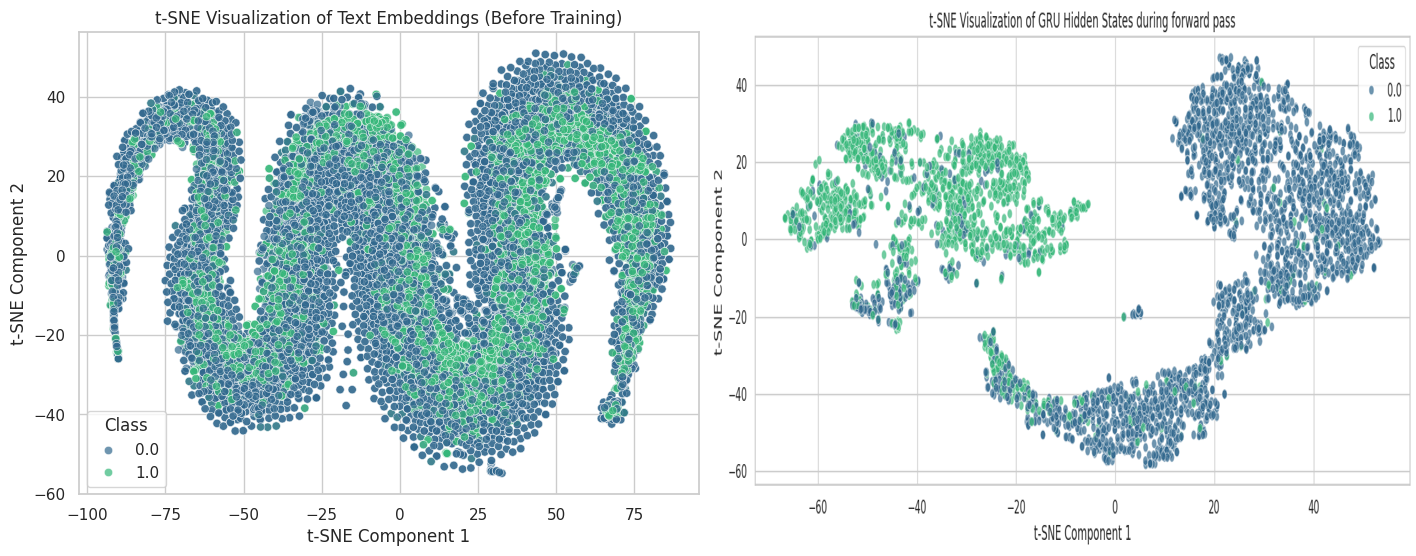
\includegraphics[width=0.7\linewidth]{No_Embeddings_GRU.png}
\caption{Projection t-SNE des représentations textuelles avant entraînement (à gauche, embeddings non ajustés) et après l'entrainement (à droite, avec le modèle GRU).}
\label{fig:tsne_gru}
\end{figure}

La figure \ref{fig:tsne_gru} illustre l’évolution des représentations au cours de l’apprentissage. À gauche, les embeddings sont initialisés aléatoirement et ne présentent aucune organisation discernable entre les classes, ce qui reflète l’absence de connaissance sémantique préalable. À droite, après passage dans le GRU entraîné, les documents sont projetés dans un espace latent où les clusters de classes apparaissent plus clairement séparés, malgré quelques zones de chevauchement.

Cela confirme que, même en partant de représentations totalement vierges, le modèle GRU parvient à construire un espace latent relativement discriminant. Les bonnes performances observées dans le tableau \ref{tab:model_performance_scratch} sont donc cohérentes avec cette transformation spatiale.

Néanmoins, malgré ces résultats prometteurs, les modèles entraînés avec des embeddings appris depuis zéro restent légèrement en retrait par rapport aux versions utilisant des embeddings pré-entraînés tels que GloVe ou FastText. Ces derniers encapsulent une structure linguistique riche issue de grands corpus, conférant une connaissance sémantique initiale que les embeddings aléatoires ne possèdent pas. En ce sens, l’intégration d’embeddings spécialisés, notamment ajustés sur des corpus biomédicaux, représenterait une piste intéressante pour améliorer encore les performances.

\subsubsection{Performances des modèles LSTM et GRU avec word embeddings : GloVe et FastText}

Les performances des modèles LSTM et GRU entraînés avec des word embeddings pré-entraînés (GloVe et FastText) sont résumées dans le tableau suivant :

\begin{table}[H]
\centering
\renewcommand{\arraystretch}{1.2}
\resizebox{1.05\textwidth}{!}{%
\begin{tabular}{|l|l|c|c|c|c|c|c|c|}
\hline
\textbf{Modèle} & \textbf{Type d'Embedding} & \textbf{Balanced Acc} & \textbf{F1 Score} & \textbf{Précision} & \textbf{Rappel} & \textbf{AUC} & \textbf{Temps Inf. (s)} & \textbf{Temps Appr. (min)} \\
\hline
LSTM & FastText (300d) & 84.27\% & 80.01\% & 83.06\% & 77.19\% & 0.95 & 0.07 & 0.85 \\
\hline
GRU & FastText (300d) & 89.96\% & 86.11\% & 81.46\% & 91.32\% & \textbf{0.97} & \textbf{0.03} & 0.43 \\
\hline
LSTM & GloVe (300d) & 89.74\% & 85.24\% & 77.85\% & \textbf{94.19\%} & 0.95 & 0.06 & 0.73 \\
\hline
GRU & GloVe (300d) & \textbf{90.70\%} & \textbf{87.75\%} & \textbf{86.53\%} & 89.01\% & 0.96 & 0.04 & \textbf{0.43} \\
\hline
\end{tabular}
}
\caption{Performances des modèles RNN avec word embeddings pré-entraînés sur l'ensemble de test.}
\label{tab:pretrained_embeddings}
\end{table}

Ces performances ont été obtenues à l’issue d’une phase d’optimisation des hyperparamètres sur l’ensemble de validation. Les configurations exactes des modèles et leurs paramètres optimaux sont disponibles en annexe dans le tableau \autoref{tab:model-config}.

L’analyse conjointe des résultats montre que les meilleures performances sont obtenues avec la combinaison GRU + GloVe. Cette configuration offre un excellent compromis entre précision (86.53\%), rappel (89.01\%) et temps d'inférence rapide (0.04s), tout en conservant un nombre modéré de paramètres (12,7M). Le taux de dropout élevé (0.8) dans ce cas agit efficacement comme régularisation, et l’optimiseur Adam combiné à un taux d’apprentissage de $1e^{-3}$ semble bien adapté. Une synthèse visuelle des résultats de performance pour ces configurations est présentée dans la figure~\ref{fig:model_performances_binary}, qui regroupe les principales métriques sous forme d’histogrammes comparatifs. Cette figure permet une lecture rapide des différences de performances entre les modèles GRU et LSTM, selon le type d’embedding utilisé (GloVe, FastText ou embeddings appris).

\begin{figure}[H]
\centering
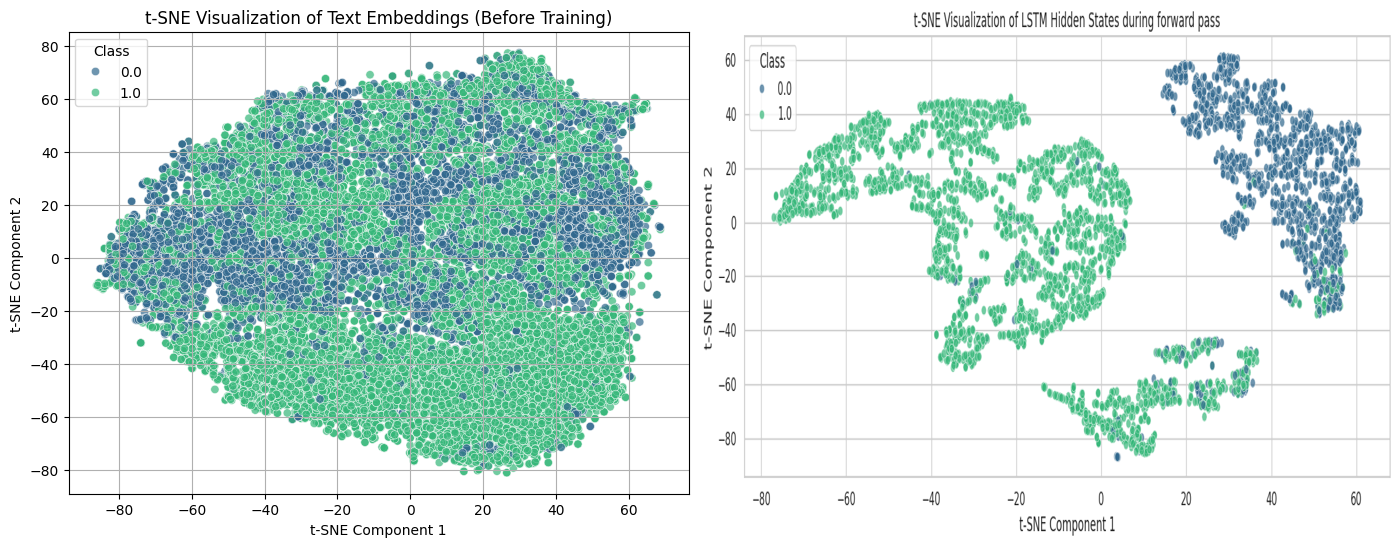
\includegraphics[width=0.7\linewidth]{Merged_Images.png}
\caption{Projection t-SNE des représentations textuelles avant entraînement (à gauche) et des états cachés du LSTM après entraînement (à droite) utilisant Glove (300d).}
\label{fig:tsne_lstm_glove}
\end{figure}

La figure \ref{fig:tsne_lstm_glove} illustre la manière dont les embeddings GloVe sont transformés par le LSTM au cours de l'entraînement. À gauche, les embeddings pré-entraînés présentent déjà une certaine organisation des classes, témoignant d’une structure sémantique initiale. À droite, après propagation dans le modèle LSTM, les représentations deviennent nettement plus discriminantes : les clusters de classes sont mieux définis, bien que quelques zones de chevauchement subsistent. Cela montre que le LSTM parvient à projeter efficacement les textes dans un espace latent où la séparation entre les classes est plus marquée.

Avant d'explorer les modèles utilisant des embeddings contextuels, il est pertinent de comparer les performances des modèles RNN lorsqu’ils apprennent les embeddings directement depuis les données, par rapport à l’utilisation de word embeddings pré-entraînés tels que GloVe ou FastText.

Les résultats présentés dans les tableaux~\ref{tab:pretrained_embeddings} et~\ref{tab:model_performance_scratch} montrent que les modèles GRU et LSTM sont capables d’apprendre des représentations lexicales efficaces directement à partir du texte brut. Par exemple, un GRU entraîné avec des embeddings appris depuis zéro atteint un F1 score de 87.11\% et une Balanced Accuracy de 90.69\%, soit des performances très proches, voire équivalentes, à celles obtenues avec des embeddings GloVe (87.75\% et 90.70\%).

En termes de précision, le GRU entraîné avec des embeddings appris (82.92\%) reste légèrement en retrait par rapport à sa version avec GloVe (86.53\%), mais compense avec un temps d’apprentissage plus court (0.37 min vs 0.43 min) et une inférence tout aussi rapide (0.04 s). Du côté du LSTM, les différences sont un peu plus marquées : le modèle avec GloVe surpasse celui avec embeddings appris sur toutes les métriques sauf le rappel, où le LSTM « from scratch » atteint un score impressionnant de 95.94\%, indiquant une très bonne capacité de détection des cas positifs.

\subsubsection{Performances des modèles GRU bidirectionnels avec l'attention de Bahdanau, les embeddings contextuels (PubMedBERT et BioBERT) et les words embeddings (Glove et FastText)}

Dans cette section, nous présentons les performances des modèles GRU bidirectionnel, noté ici \texttt{BiGRU}, utilisant des embeddings contextuels spécialisés, à savoir \gls{pubmedbert} et \gls{biobert}, qui ont été préalablement entraînés sur des corpus biomédicaux. Ces modèles sont particulièrement adaptés aux tâches de classification dans le domaine de la santé, car ils intègrent une compréhension fine du vocabulaire et des relations sémantiques propres au domaine biomédical.

Les résultats des différentes configurations du modèle BiGRU avec les embeddings GloVe, FastText, PubMedBERT et BioBERT sont synthétisés dans le tableau~\ref{tab:biGRU_performance_contextual_embeddings}.

\begin{table}[H]
\centering
\renewcommand{\arraystretch}{1.2}
\resizebox{1.05\textwidth}{!}{%
\begin{tabular}{|l|l|c|c|c|c|c|c|c|}
\hline
\textbf{Modèle} & \textbf{Type d'Embedding} & \textbf{Balanced Acc} & \textbf{F1 Score} & \textbf{Précision} & \textbf{Rappel} & \textbf{AUC} & \textbf{Temps Inf. (s)} & \textbf{Temps Appr. (min)} \\
\hline
BiGRU + Bahdanau & GloVe (300d) & 95.78\% & 96.50\% & 96.49\% & 96.50\% & 0.99 & 0.05 & 4.96 \\
\hline
BiGRU + Bahdanau & FastText (300d) & 96.02\% & 96.91\% & \textbf{96.93\%} & 96.93\% & 0.99 & 0.04 & 4.45 \\
\hline
BiGRU + Bahdanau & PubMedBERT (768d) & 96.09\% & 97.72\% & 97.05\% & \textbf{98.40\%} & \textbf{1.00} & 1.67 & 68.83 \\
\hline
BiGRU + Bahdanau & BioBERT (768d) & \textbf{96.10\%} & \textbf{98.00\%} & 97.00\% & 98.00\% & 0.99 & 1.68 & \textbf{70.37} \\
\hline
\end{tabular}
}
\caption{Performances des modèles BiGRU avec différents embeddings sur l'ensemble de test.}
\label{tab:biGRU_performance_contextual_embeddings}
\end{table}

Les résultats obtenus montrent des performances remarquables pour les modèles (dont les hyperparamètres sont précisés dans le tableau~\ref{tab:model-config}) utilisant des embeddings contextuels, en particulier \gls{biobert} et \gls{pubmedbert}. Ces configurations surpassent nettement les versions utilisant des embeddings classiques comme GloVe ou FastText.

Le modèle \textit{BiGRU + BioBERT} atteint un F1 score de 98.00\%, avec une précision de 97.00\% et un rappel de 98.00\%, illustrant une très grande capacité à détecter les classes positives, un aspect essentiel dans les applications biomédicales. Le modèle \textit{BiGRU + PubMedBERT}, quant à lui, enregistre un F1 score de 97.72\%, avec un rappel légèrement supérieur (98.40\%).

Il est particulièrement intéressant de comparer ces deux modèles en tenant compte non seulement de leurs performances, mais aussi de leur complexité et de leur mode d'intégration. En effet, dans le cas du modèle basé sur PubMedBERT, l'encodeur BERT a été utilisé en tant que composant gelé, c’est-à-dire que ses poids n'ont pas été mis à jour durant l'entraînement du modèle BiGRU. Cela se reflète directement dans le nombre total de paramètres entraînables : seulement \textbf{1,708,033} pour \textit{BiGRU + PubMedBERT}, contre \textbf{110,018,305} pour \textit{BiGRU + BioBERT}, dans lequel l’encodeur BERT a été fine-tuné conjointement avec le reste du modèle. Cette distinction est cruciale pour évaluer le coût réel de l'apprentissage et la capacité du modèle à s’adapter à la tâche cible.

Par ailleurs, cette architecture gelée de PubMedBERT a initialement été testée dans le cadre d’une classification binaire, où elle a permis d’identifier clairement l’impact de l'entraînement (ou non) des couches BERT sur les métriques finales, mais aussi sur les temps d’entraînement et d’inférence. Les résultats de cette évaluation sont présentés dans la figure~\ref{fig:model_performances_binary}, qui compare directement les performances des différentes configurations de modèles dans ce cadre binaire.

Enfin, il est important de noter que les représentations issues des modèles BERT sont déjà organisées de manière structurelle, comme le confirment les visualisations par t-SNE (voir figure~\ref{fig:tsne_lstm_glove}). Cette structure facilite la séparation des classes même avant fine-tuning, à la différence des embeddings appris depuis zéro où aucune organisation claire n’apparaît initialement (figure~\ref{fig:tsne_gru}).

Les deux modèles contextuels présentent un AUC très élevé : 0.99 pour BioBERT et 1.00 pour PubMedBERT, attestant de leur grande capacité de discrimination. En contrepartie, leur temps d'entraînement est significativement plus long (environ 70 minutes), bien que leur temps d’inférence (1.67 secondes) reste acceptable pour des applications en environnement clinique.

En résumé, cette analyse comparative montre que, malgré un coût computationnel nettement plus élevé, les modèles basés sur des embeddings contextuels spécialisés comme BioBERT (fine-tuné) offrent les meilleures performances. Toutefois, l’approche avec PubMedBERT gelé constitue une alternative viable dans des contextes où les ressources sont limitées, tout en bénéficiant de l'efficacité du langage pré-entraîné.

\subsection{Étude de l’impact du déséquilibre des classes : rééchantillonnage et pondération des pertes}

Dans le contexte de la classification de textes biomédicaux, le déséquilibre des classes peut fortement affecter les performances des modèles, en particulier sur les classes minoritaires. Or, certains modèles performants, notamment ceux basés sur des embeddings contextuels, sont très coûteux en ressources computationnelles, ce qui limite leur accessibilité et leur utilisation pratique dans certains contextes.

Afin d’examiner si des méthodes classiques de lutte contre le déséquilibre telles que le rééchantillonnage (\gls{smote}, Borderline-\gls{smote}) ou la pondération des classes dans la fonction de perte peuvent améliorer les performances, nous évaluons ici leur impact à la fois sur la qualité des prédictions (métriques d’évaluation) mais aussi sur les coûts d’entraînement et d’inférence. Cette analyse est cruciale pour déterminer si des techniques plus légères peuvent constituer une alternative intéressante, notamment lorsque les ressources disponibles sont limitées ou que l’utilisation de modèles lourds n’est pas envisageable.

Nous nous concentrons particulièrement sur les architectures LSTM et GRU avec embeddings appris depuis zéro (section~4.6.1.1), puis sur celles utilisant des embeddings statiques pré-entraînés comme GloVe et FastText (section~4.6.1.2), afin d’évaluer la pertinence et l’efficacité de ces méthodes de gestion du déséquilibre dans des contextes aux contraintes computationnelles variées.

\begin{table}[H]
\centering
\scriptsize
\caption{Performance of LSTM and GRU models with different resampling and weighting strategies (binary classification)}
\begin{tabular}{|l|l|c|c|c|c|}
\hline
\textbf{Training Strategy} & \textbf{Model} & \textbf{Accuracy} & \textbf{F1-score} & \textbf{Balanced Acc} & \textbf{Recall} \\
\hline
No resampling & LSTM & 90.70\% & 87.23\% & 90.46\% & 89.64\% \\
No resampling & GRU  & 91.74\% & 88.76\% & 91.81\% & 92.02\% \\
\hline
SMOTE & LSTM & 89.66\% & 86.40\% & 90.35\% & 92.72\% \\
SMOTE & GRU  & \textbf{92.04\%} & \textbf{89.09\%} & \textbf{91.96\%} & 91.67\% \\
\hline
Borderline-SMOTE & LSTM & 90.45\% & 87.25\% & 90.84\% & 92.16\% \\
Borderline-SMOTE & GRU  & 90.92\% & 87.87\% & 91.35\% & 92.79\% \\
\hline
Class Weights & LSTM & 90.13\% & 87.32\% & 91.43\% & \textbf{95.87\%} \\
Class Weights & GRU  & 91.97\% & 88.83\% & 91.55\% & 90.13\% \\
\hline
\end{tabular}
\label{tab:performance_resampling}
\end{table}

La \textbf{Table~\ref{tab:performance_resampling}} présente les performances des modèles LSTM et GRU entraînés selon différentes stratégies de gestion du déséquilibre des classes, notamment par rééchantillonnage (\textit{SMOTE}, \textit{Borderline-SMOTE}) et par pondération des classes dans la fonction de perte. Ces résultats sont également synthétisés visuellement dans la figure~\ref{fig:resampling}, qui met en évidence les effets de ces techniques sur les principales métriques de performance.

On observe que ces méthodes permettent d’améliorer certaines métriques clés, en particulier le rappel des classes minoritaires, sans compromettre la performance globale. Par exemple, le modèle GRU associé à SMOTE atteint une F1-score de 89.09\%et un rappel de 91.67\%, traduisant un bon équilibre entre précision et sensibilité. De même, le LSTM avec pondération des classes obtient un rappel exceptionnel de 95.87\%, ce qui est crucial dans des scénarios où la détection des cas rares est prioritaire.

Par ailleurs, les temps d’entraînement et d’inférence demeurent comparables aux versions de base (cf. sections~4.6.1.1 et~4.6.1.2), ce qui montre que ces techniques n'engendrent pas de surcoût computationnel significatif, et peuvent donc être facilement intégrées à des pipelines existants, y compris dans des environnements contraints.

Cependant, les gains observés avec SMOTE restent relativement modestes au regard de son potentiel théorique. Cette limite peut s'expliquer à la lumière des visualisations t-SNE (Figures~\ref{fig:tsne_gru} et~\ref{fig:tsne_lstm_glove}). Celles-ci révèlent que, bien que les modèles GRU et LSTM parviennent à structurer un espace latent relativement discriminant, des zones de chevauchement entre classes subsistent. Or, SMOTE repose sur l’hypothèse que les exemples proches dans l’espace des représentations appartiennent à la même classe, ce qui n’est pas toujours vrai dans des configurations à forte ambiguïté sémantique. En interpolant dans ces zones frontières, SMOTE peut involontairement générer des exemples ambigus, nuisant à l’apprentissage plutôt que de le renforcer.

En définitive, les approches par rééchantillonnage et pondération constituent des solutions simples, peu coûteuses et efficaces pour atténuer l’impact du déséquilibre, en particulier dans les cas où l’usage de modèles à embeddings contextuels lourds est prohibitif. Leur intégration se justifie d’autant plus qu’elles s’appuient sur des mécanismes génériques, adaptables à divers modèles et jeux de données.

\subsection{Apprentissage par petites touches (Few-Shot Learning)}

L’apprentissage par petites touches, ou \gls{fsl}, constitue une approche prometteuse dans les contextes à faibles ressources, en particulier pour la classification de maladies rares. Cette section évalue les capacités de généralisation de plusieurs modèles de classification \textit{binaire} lorsqu’ils sont entraînés avec un nombre limité d’exemples par classe (\textit{k-shot}).

Dans le cadre de notre investigation sur la capacité des modèles à \textit{généraliser} dans des conditions de données limitées, nous avons exceptionnellement introduit un modèle supplémentaire, \textit{CNN+LSTM}, combinant des couches convolutionnelles et récurrentes. Ce choix visait à accroître la complexité architecturale des modèles testés, afin d’explorer dans quelle mesure une structure plus expressive pouvait améliorer la généralisation en few-shot learning.

La Figure~\ref{fig:kshot_binary} illustre les performances comparées de plusieurs architectures sur cinq métriques : F1-score, Balanced Accuracy, Recall, Précision et Accuracy sur l’ensemble de test. Chaque ligne correspond à un modèle différent, et chaque colonne à une métrique. Ces résultats permettent d’analyser la stabilité, l’évolution avec $k$ et la performance globale de chaque approche.

Le modèle \textit{GRU-FastText} présente des résultats très faibles et peu évolutifs. F1, Recall et Balanced Accuracy stagnent autour de 0.2 à 0.3, quelle que soit la valeur de $k$, traduisant une incapacité du modèle à exploiter les faibles quantités d’exemples. Le modèle \textit{GRU-GloVe} ne fait pas mieux, montrant une instabilité importante et des métriques proches du hasard.

Le \textit{CNN+LSTM} est légèrement plus stable, avec une progression marginale pour les plus grands $k$, mais reste insuffisant avec un F1 inférieur à 0.25 même à $k=500$. Ce résultat suggère que, malgré sa complexité accrue, cette architecture n’est pas nécessairement mieux adaptée au contexte de few-shot learning binaire.

Le modèle \textit{GRU-BaselineFastText} affiche une amélioration progressive avec $k$, surtout en Recall et F1, bien que les valeurs absolues restent modestes (inférieures à 0.4).

Le modèle \textit{GRU-BaselineGloVe}, quant à lui, se démarque clairement. Il montre une progression régulière sur toutes les métriques, atteignant un F1 supérieur à 0.7 et une Balanced Accuracy proche de 0.9 pour $k=500$, ce qui suggère une bonne aptitude à généraliser à partir de peu d’exemples.

Ces tendances sont confirmées par la Figure~\ref{fig:kshot_binary_bi_Gru}, qui se concentre plus précisément sur le modèle \textit{BiGRU avec mécanisme d’attention de Bahdanau et embeddings GloVe}. On y observe la diminution progressive de la perte, accompagnée d’une amélioration constante du F1-score et de la Balanced Accuracy sur l’ensemble de test, en fonction de $k$. Cela illustre non seulement la stabilité de ce modèle, mais aussi sa robustesse dans des contextes à faibles ressources.

Ces résultats soulignent que dans des scénarios à faibles ressources, seuls certains modèles — notamment ceux dotés d’architectures avancées et de représentations lexicales spécialisées — parviennent à \textit{généraliser efficacement}. Le modèle \textit{BiGRU avec attention}, lorsqu’il est associé à GloVe, s’impose comme un candidat robuste pour la classification binaire biomédicale, même dans des conditions où les données étiquetées sont rares.

\subsection{Résultats expérimentaux de la classification multiclasses}

\subsubsection{Performances des modèles LSTM, GRU, CNN+LSTM et CNN+GRU avec embeddings appris depuis zéro}

Les performances des modèles CNN+LSTM, CNN+GRU, LSTM et GRU, entraînés avec des embeddings appris depuis zéro, sont présentées dans le tableau~\ref{tab:performances_multiclass} et sur ~\ref{fig:auc_multi}. Les hyperparamètres optimaux retenus pour chaque modèle sont détaillés dans le tableau~\ref{tab:hyperparams_multiclass}.

\begin{table}[H]
\centering
\resizebox{\textwidth}{!}           & \textbf{88.36\%}           & 88.40\%              & \textbf{89.34\%}            & \textbf{88.13\%}         & 22.85                    & 0.04                         \\ \hline
CNN+GRU            & Learned (from scratch, Raw Text, 250d)    & 86.77\%           & 87.11\%           & 87.09\%              & 88.35\%            & 86.77\%         & 13.38                    & \textbf{0.02}                         \\ \hline
LSTM               & Learned (from scratch, Raw Text, 250d)    & \textbf{88.13\%}           & \textbf{88.36\%}           & \textbf{88.46\%}              & 88.88\%            & \textbf{88.13\%}         & \textbf{9.03}                     & 0.07                         \\ \hline
GRU                & Learned (from scratch, Raw Text, 250d)    & 87.74\%           & 87.78\%           & 88.00\%              & 88.00\%            & 87.74\%         & 9.09                     & 0.03                         \\ \hline
\end{tabular}
}
\caption{Performances des modèles avec embeddings appris depuis zéro sur l’ensemble de test en classification multiclasses.}
\label{tab:performances_multiclass}
\end{table}

Ces résultats montrent que les modèles CNN+LSTM et LSTM obtiennent les meilleures performances en termes d’exactitude et de F-1 score, proches de 88\%. Le modèle GRU, bien que légèrement moins performant, reste compétitif, notamment grâce à des temps d’entraînement et d’inférence plus courts. Le modèle CNN+GRU est quant à lui le plus rapide à l’inférence, au prix d’une légère baisse de performance.

\begin{figure}[H]
\centering
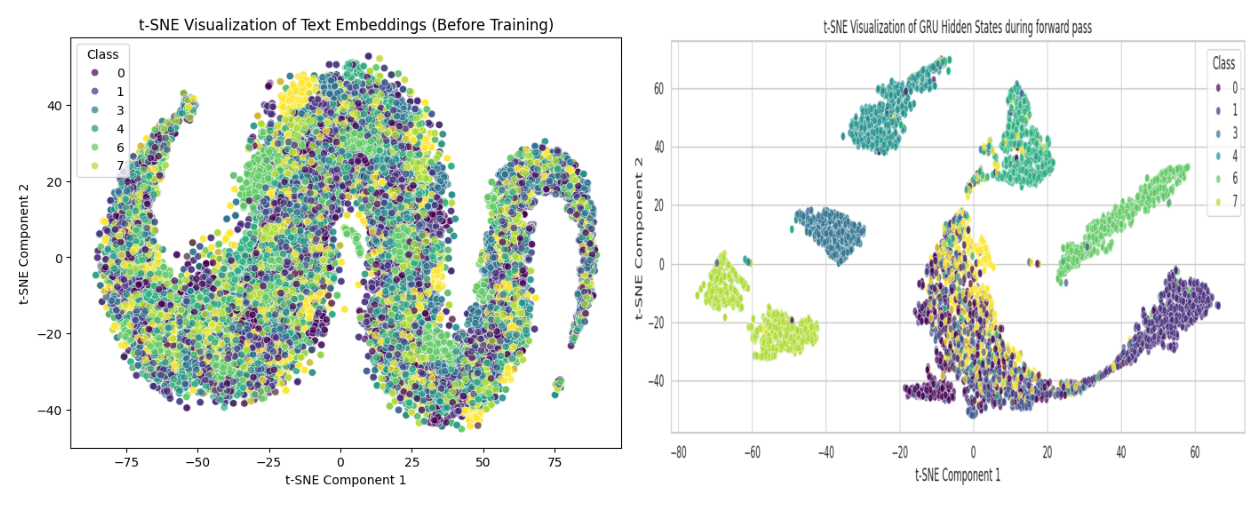
\includegraphics[width=0.7\linewidth]{no_embed_Multi_tsne_gru.png}
\caption{Projection t-SNE des représentations textuelles avant entraînement (à gauche, embeddings non ajustés) et après entraînement (à droite, avec le modèle GRU) en classification multiclasses.}
\label{fig:no_embed_Multi_tsne_gru}
\end{figure}

La figure~\ref{fig:gru_multi_tsne} présente la projection t-SNE des représentations textuelles avant entraînement (à gauche, embeddings non ajustés) et après entraînement (à droite, avec le modèle GRU) en classification multiclasses utilisant les embeddings GloVe (300d). Avant entraînement, les représentations initiales apparaissent peu structurées, avec un mélange important des différentes classes. Après entraînement, les états cachés du GRU se regroupent en clusters plus nets, traduisant une meilleure séparation des classes malgré quelques chevauchements résiduels. Les performances des modèles LSTM, GRU, CNN+LSTM et CNN+GRU exploitant ces embeddings pré-entraînés sont détaillées dans le tableau~\ref{tab:performances_pretrained}, où les meilleures valeurs sont mises en évidence en gras. Ces résultats sont également illustrés sous forme d’histogrammes dans la figure~\ref{fig:multi_class_performance}.

Ces observations confirment que, même en partant d’embeddings appris depuis zéro, les modèles étudiés sont capables d’apprendre des représentations discriminantes adaptées à la classification multiclasses. Toutefois, l’intégration d’embeddings pré-entraînés pourrait encore améliorer la qualité de la séparation des classes.

Bien que ces résultats soient encourageants, il convient de noter que les modèles entraînés exclusivement avec des embeddings appris depuis zéro ne bénéficient pas des connaissances linguistiques préalables présentes dans des embeddings pré-entraînés tels que GloVe ou FastText. Ces derniers intègrent une richesse sémantique issue de larges corpus textuels, conférant ainsi une meilleure capacité initiale à distinguer les classes. Dans cette optique, la prochaine section explore les performances des modèles lorsque des embeddings pré-entraînés sont utilisés, afin d’évaluer leur impact sur la classification multiclasses.

\subsubsection{Performances des modèles LSTM, GRU, CNN+LSTM et CNN+GRU avec word embeddings : GloVe et FastText}

Les performances des modèles CNN+LSTM, CNN+GRU, LSTM et GRU utilisant des embeddings pré-entraînés GloVe et FastText (300 dimensions) sont présentées dans le tableau~\ref{tab:performances_pretrained}. Les configurations d’hyperparamètres optimales sont celles détaillées dans la section précédente (cf. tableau~\ref{tab:hyperparams_multiclass}).

\begin{table}[H]
\centering
\resizebox{\textwidth}{!}           & \textbf{90.49\%}           & \textbf{90.73\%}              & \textbf{90.58\%}            & \textbf{90.50\%}         & \textbf{5.12}                     & 0.06                         \\ \hline
CNN+GRU            & FastText (300d)           & 88.91\%           & 88.96\%           & 89.15\%              & 89.15\%            & 88.91\%         & 8.25                     & 0.03                         \\ \hline
LSTM               & FastText (300d)           & 80.49\%           & 80.65\%           & 81.67\%              & 89.21\%            & 80.49\%         & $\sim$11.0               & 0.09                         \\ \hline
GRU                & FastText (300d)           & 92.26\%           & 92.26\%           & 92.46\%              & 92.31\%            & 92.26\%         & 2.67                     & \textbf{0.06}                         \\ \hline
CNN+LSTM           & GloVe (300d)              & 87.19\%           & 87.60\%           & 87.43\%              & 89.16\%            & 87.19\%         & 19.28                    & 0.06                         \\ \hline
CNN+GRU            & GloVe (300d)              & 87.62\%           & 87.72\%           & 87.89\%              & 88.33\%            & 87.62\%         & 12.74                    & 0.03                         \\ \hline
LSTM               & GloVe (300d)              & 89.17\%           & 89.25\%           & 89.51\%              & 89.51\%            & 89.17\%         & 41.73                    & 0.05                         \\ \hline
\end{tabular}
}
\caption{Performances des modèles avec embeddings pré-entraînés GloVe et FastText sur l’ensemble de test en classification multiclasses.}
\label{tab:performances_pretrained}
\end{table}

La figure~\ref{fig:gru_multi_tsne} illustre la projection t-SNE des représentations textuelles avant et après entraînement du modèle GRU utilisant des embeddings GloVe (300d). Avant entraînement, les embeddings initiaux apparaissent peu structurés, sans séparation nette entre les classes. En revanche, après entraînement, les états cachés du GRU s’organisent en clusters bien distincts, ce qui traduit l’acquisition de représentations internes discriminantes, efficaces pour la classification multiclasses.

\begin{figure}[H]
\centering
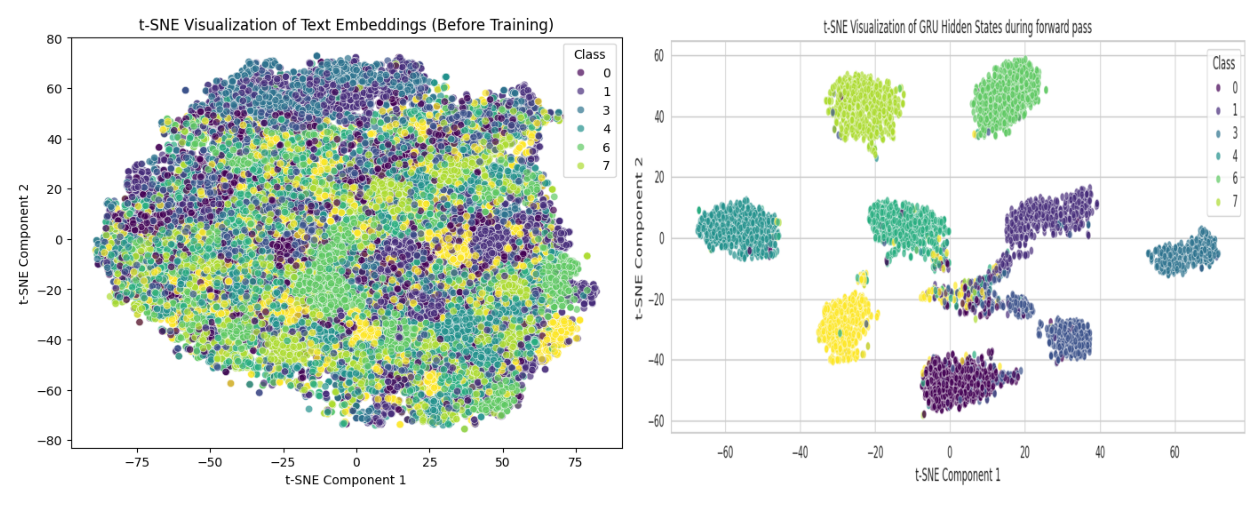
\includegraphics[width=0.7\linewidth]{gru_multi_tsne.png}
\caption{Projection t-SNE des représentations textuelles avant entraînement (à gauche, embeddings non ajustés) et après entraînement (à droite, avec le modèle GRU) en classification multiclasses utilisant GloVe (300d).}
\label{fig:gru_multi_tsne}
\end{figure}

Les résultats montrent que le modèle GRU associé aux embeddings FastText atteint les meilleures performances en termes d’exactitude (92.26\%), de F1-score et d’exactitude équilibrée, surpassant ainsi les autres architectures. Le CNN+LSTM avec FastText affiche également d’excellentes métriques, se positionnant juste derrière le GRU tout en bénéficiant d’un temps d’entraînement très réduit (5.12 minutes), ce qui représente un compromis intéressant entre précision et coût computationnel. On peut également voir ces résultats sous forme d'histogrammes via la figure~\ref{fig:multi_class_performance} et sur et sur ~\ref{fig:auc_multi}.

Les modèles utilisant GloVe présentent globalement des performances légèrement inférieures à celles obtenues avec FastText, avec notamment un temps d’entraînement plus élevé, en particulier pour le LSTM (près de 42 minutes). En termes de temps d’inférence, le CNN+GRU et le GRU sont les plus rapides, affichant des durées inférieures à 0.06 seconde, ce qui peut être un critère déterminant dans des contextes où la rapidité de prédiction est cruciale.

Il est également intéressant de noter que, comparés aux modèles entraînés \textit{from scratch}, ceux utilisant des word embeddings pré-entraînés (GloVe ou FastText) bénéficient d’une meilleure convergence et d’une généralisation plus stable, tout en réduisant la nécessité d’un entraînement long sur des jeux de données spécifiques.Cette approche permet aux modèles de s’appuyer sur des représentations linguistiques déjà riches, ce qui améliore notablement leurs performances sur des tâches complexes comme la classification multiclasses. Ces résultats motivent l’exploration de méthodes encore plus sophistiquées, en particulier les modèles basés sur des embeddings contextuels tels que ceux issus de PubMedBERT et BioBERT.

\subsubsection{Performances des modèles GRU bidirectionnels avec l'attention de Bahdanau, les embeddings contextuels (PubMedBERT et BioBERT) et les word embeddings (GloVe et FastText)}

Les résultats précédents ont montré l’intérêt des embeddings pré-entraînés statiques, tels que FastText et GloVe, pour améliorer les performances des modèles séquentiels classiques. Pour aller plus loin, cette section évalue l’impact des représentations contextuelles issues de modèles de langage de type BERT, spécifiquement adaptés au domaine biomédical, à savoir PubMedBERT et BioBERT. Ces représentations contextuelles sont intégrées dans une architecture BiGRU enrichie d’une couche d’attention de type Bahdanau, permettant de mieux capter les relations contextuelles dans les séquences textuelles.

Les hyperparamètres retenus pour ces modèles correspondent à ceux optimisés lors de la phase de réglage détaillée précédemment (cf. tableau~\ref{tab:hyperparams_multiclass}).

\begin{table}[H]
\centering
\resizebox{\textwidth}{!}{%
\begin{tabular}{|l|l|c|c|c|c|c|c|c|}
\hline
\textbf{Modèle}             & \textbf{Type d'Embedding} & \textbf{Exactitude} & \textbf{F1 Score} & \textbf{Exactitude équilibrée} & \textbf{Précision} & \textbf{Rappel} & \textbf{Temps d'entraînement (min)} & \textbf{Temps d'inférence (s)} \\ \hline
\textbf{BiGRU + Bahdanau}   & GloVe (300d)              & 92.17\%           & 92.21\%           & 92.35\%              & 92.40\%            & 92.17\%         & 10.56                    & 0.21                         \\ \hline
\textbf{BiGRU + Bahdanau}   & FastText (300d)           & 92.80\%           & 92.89\%           & 93.04\%              & 93.14\%            & 92.80\%         & 9.96                     & 0.22                         \\ \hline
\textbf{BiGRU + Bahdanau}   & PubMedBERT                & 91.89\%           & 91.90\%           & 92.16\%              & 91.96\%            & 91.89\%         & 33.33                    & 0.50                         \\ \hline
\textbf{BiGRU + Bahdanau}   & BioBERT                   & \textbf{92.23\%}  & \textbf{92.33\%}  & \textbf{92.01\%}     & \textbf{92.13\%}    & \textbf{92.21\%} & 35.66                    & 0.49                         \\ \hline
\end{tabular}
}
\caption{Performances des modèles BiGRU avec attention et différents types d'embeddings (statiques et contextuels) sur l’ensemble de test.}
\label{tab:performances_contextual}
\end{table}

La figure~\ref{fig:gru_multi_tsne} illustre la projection t-SNE des représentations extraites du modèle \textit{BiGRU + BioBERT} avant et après entraînement. Avant entraînement, les vecteurs issus de l’encodeur BERT gelé présentent une structure peu discriminante, avec un mélange important des classes. Après entraînement, les représentations apprises montrent une séparation nettement plus marquée entre les différentes classes, traduisant une meilleure adaptation du modèle à la tâche de classification multiclasses, et surpassant la séparation observée avec les embeddings statiques tels que GloVe.

Les résultats reportés dans le tableau~\ref{tab:performances_contextual} et sur ~\ref{fig:auc_multi} confirment les bénéfices des embeddings contextuels, en particulier avec BioBERT. Le modèle \textit{BiGRU + BioBERT}, dont l’encodeur est fine-tuné conjointement avec le reste du réseau, obtient les meilleures performances globales, notamment en F1-score (92.33\%) et précision (92.13\%). Toutefois, ce gain de performance s’accompagne d’un coût computationnel significatif, avec un temps d’entraînement dépassant 35 minutes et un temps d’inférence proche de 0.5 seconde par échantillon.

En comparaison, le modèle \textit{BiGRU + PubMedBERT}, qui utilise un encodeur BERT gelé — c’est-à-dire sans mise à jour des poids durant l’entraînement — affiche un nombre nettement plus faible de paramètres entraînables (\textbf{1,708,033} contre \textbf{110,018,305} pour BioBERT). Ce choix limite la capacité du modèle à s’adapter finement à la tâche, ce qui se traduit par des performances légèrement inférieures, mais avec un coût en temps et en ressources plus modéré.

Pour une meilleure visualisation et comparaison des différentes métriques d’évaluation (exactitude équilibrée, F1-score, précision et rappel), la figure~\ref{fig:multi_class_performance} présente un résumé sous forme d’histogrammes des performances obtenues par chacun des modèles testés.

En synthèse, les modèles basés sur BioBERT offrent un compromis optimal entre précision et expressivité, au prix d’une complexité et d’un temps d’entraînement plus élevés. Les variantes utilisant PubMedBERT proposent une alternative plus légère, convenant mieux aux contraintes computationnelles, mais avec un léger compromis sur la qualité prédictive. Les modèles reposant sur les embeddings statiques restent néanmoins compétitifs, particulièrement lorsqu’un compromis entre performance et rapidité est recherché.

\subsection{Étude de l’impact du déséquilibre des classes : rééchantillonnage et pondération des pertes}

Dans le cadre de la classification de textes biomédicaux, les déséquilibres entre classes peuvent avoir un impact considérable sur la qualité des prédictions, notamment en réduisant la capacité des modèles à bien généraliser sur les classes minoritaires. Cette problématique est d’autant plus critique que les modèles les plus performants reposent souvent sur des architectures lourdes, telles que les encodeurs contextuels de type BERT, dont le coût computationnel limite l’applicabilité dans des environnements contraints en ressources.

Dans cette optique, nous explorons ici l’efficacité de stratégies classiques de traitement du déséquilibre : le rééchantillonnage des données (via SMOTE et Borderline-SMOTE) ainsi que la pondération des classes dans la fonction de perte (weighted training). L’objectif est double : évaluer dans quelle mesure ces approches permettent d’améliorer les performances sur l’ensemble des classes, tout en analysant si elles constituent une alternative efficace et moins coûteuse à l’utilisation de modèles massivement pré-entraînés.

Pour cela, nous avons comparé les performances du modèle \textit{BiGRU} avec attention de Bahdanau, en combinaison avec différents types d’embeddings (GloVe, FastText, PubMedBERT et BioBERT), selon quatre stratégies d’apprentissage différentes : sans rééquilibrage, avec SMOTE, avec Borderline-SMOTE, et avec pondération des classes dans la fonction de perte. Le tableau \ref{tab:performance_multiclass} présente la synthèse des résultats obtenus, en termes d’exactitude, d’exactitude équilibrée, de F1-score, de précision et de rappel, pour chaque combinaison testée.

\begin{table}[H]
    \centering
    \scriptsize
    \caption{Performance comparison of models using SMOTE, Borderline-SMOTE, and Weighted Training (Multi-Class Classification)}
    \label{tab:performance_multiclass}
    \begin{tabular}{|l|l|l|c|c|c|c|c|}
    \hline
    \textbf{Training Strategy} & \textbf{Model} & \textbf{Embedding} & \textbf{Accuracy} & \textbf{Balanced Acc} & \textbf{F1-score} & \textbf{Precision} & \textbf{Recall} \\
    \hline
    No resampling & BiGRU+Bahdanau & GloVe (300d)     & 92.17\% & 92.35\% & 92.21\% & 92.40\% & 92.17\% \\
    No resampling & BiGRU+Bahdanau & FastText (300d)  & \textbf{92.80\%} & 93.04\% & \textbf{92.89\%} & \textbf{93.14\%} & \textbf{92.80\%} \\
    No resampling & BiGRU+Bahdanau & PubMedBERT       & 91.89\% & 92.16\% & 91.90\% & 91.96\% & 91.89\% \\
    \hline
    SMOTE         & BiGRU+Bahdanau & GloVe (300d)     & 90.60\% & 90.88\% & 90.58\% & 90.58\% & 90.60\% \\
    SMOTE         & BiGRU+Bahdanau & FastText (300d)  & 91.45\% & 91.71\% & 91.49\% & 91.59\% & 91.45\% \\
    SMOTE         & BiGRU+Bahdanau & PubMedBERT       & 92.38\% & 92.56\% & 92.36\% & 92.48\% & 92.38\% \\
    SMOTE         & BiGRU+Bahdanau & BioBERT          & 92.00\% & 92.00\% & 92.00\% & \textbf{93.00\%} & 92.00\% \\
    \hline
    Borderline-SMOTE & BiGRU+Bahdanau & GloVe (300d)   & 90.84\% & 91.09\% & 90.84\% & 90.86\% & 90.84\% \\
    Borderline-SMOTE & BiGRU+Bahdanau & FastText (300d)& 91.89\% & 92.16\% & 91.90\% & 91.96\% & 91.89\% \\
    Borderline-SMOTE & BiGRU+Bahdanau & PubMedBERT    & 92.07\% & 92.18\% & 92.02\% & 92.19\% & 92.07\% \\
    Borderline-SMOTE & BiGRU+Bahdanau & BioBERT       & 92.00\% & 92.00\% & 92.00\% & \textbf{93.00\%} & 92.00\% \\
    \hline
    Weighted Training & BiGRU+Bahdanau & GloVe (300d)  & 90.29\% & 90.54\% & 90.35\% & 90.51\% & 90.29\% \\
    Weighted Training & BiGRU+Bahdanau & FastText (300d)& 92.17\% & 92.43\% & 92.19\% & 92.32\% & 92.17\% \\
    Weighted Training & BiGRU+Bahdanau & PubMedBERT    & 92.33\% & \textbf{92.57\%} & 92.31\% & 92.32\% & 92.33\% \\
    Weighted Training & BiGRU+Bahdanau & BioBERT       & 92.00\% & \textbf{93.00\%} & 92.00\% & \textbf{93.00\%} & 92.00\% \\
    \hline
    \end{tabular}
\end{table}

L’analyse comparative met en évidence plusieurs tendances significatives. Tout d’abord, les résultats obtenus sans aucune méthode de rééquilibrage restent très compétitifs, en particulier avec les embeddings statiques. Le modèle \textit{BiGRU + FastText} se démarque avec une F1-score de 92,89\% et une précision de 93,14\%, constituant ainsi la meilleure configuration de base sans recours à des stratégies d’équilibrage.

L'application de la méthode SMOTE montre des effets contrastés. Si elle améliore légèrement les performances des modèles utilisant des embeddings contextuels, comme PubMedBERT (F1-score de 92,36\% contre 91,90\% sans rééchantillonnage), elle tend en revanche à dégrader celles obtenues avec des embeddings statiques. Par exemple, le modèle \textit{BiGRU + GloVe} voit sa F1-score chuter de 92,21\% à 90,58\%. Cela suggère que SMOTE, reposant sur une interpolation linéaire dans l’espace des caractéristiques, est moins adapté aux représentations fortement corrélées ou denses comme celles générées par GloVe ou FastText.

Cette hypothèse est corroborée par les visualisations t-SNE présentées précédemment. Celles-ci révèlent que les représentations statiques, notamment avec GloVe, génèrent des regroupements compacts avec des frontières de classes parfois floues, rendant l’injection d’exemples synthétiques potentiellement perturbatrice. À l’inverse, les embeddings contextuels comme ceux de PubMedBERT offrent une structuration plus diffuse de l’espace sémantique, avec des séparations de classes plus marquées. Dans ce cas, SMOTE et Borderline-SMOTE peuvent produire des exemples synthétiques plus cohérents et utiles au modèle, en particulier lorsqu’ils sont concentrés sur les zones de frontière.

Borderline-SMOTE, plus prudent dans la génération de données en se focalisant sur les régions proches des décisions limites, s'avère ainsi légèrement plus efficace que SMOTE classique, notamment en association avec FastText ou PubMedBERT. Toutefois, les gains restent marginaux et ne dépassent pas les meilleures performances obtenues sans rééchantillonnage.

À l’inverse, la pondération des classes dans la fonction de perte (weighted training) se distingue par sa robustesse et sa cohérence. Cette approche permet non seulement de maintenir les performances des modèles plus légers, mais également d’optimiser celles des modèles à base d’encodeurs contextuels. Le modèle \textit{BiGRU + PubMedBERT} atteint ainsi une balanced accuracy de 92,57\% (la plus élevée pour ce modèle) et une F1-score de 92,31\%. De même, la configuration \textit{BiGRU + BioBERT}, avec pondération, atteint une précision remarquable de 93,00\% tout en conservant une performance globale stable.

Ces résultats indiquent que la pondération des classes constitue une solution simple, stable et efficace pour améliorer la détection des classes minoritaires, sans recourir à la génération artificielle de données. Elle n’implique aucun coût additionnel notable en termes de temps d’entraînement ou de complexité architecturale, ce qui la rend particulièrement adaptée aux environnements contraints.

En conclusion, si les méthodes de rééchantillonnage peuvent présenter un intérêt dans certains cas spécifiques — notamment avec des embeddings contextuels bien structurés — elles n’égalent pas, dans notre cadre expérimental, les performances offertes par les stratégies de pondération. Ces dernières s’imposent comme un compromis optimal entre efficacité, stabilité et sobriété computationnelle, en particulier lorsqu’elles sont appliquées à des modèles contextuels comme PubMedBERT ou BioBERT.

\subsection{Apprentissage par petites touches (Few-Shot Learning)}

Tout comme cela a été réalisé dans le cas de la classification \textit{binaire}, nous explorons ici les performances des modèles dans un contexte de \textit{few-shot learning} appliqué à la classification \textit{multi-classes}. L'objectif est d'évaluer la capacité des différentes architectures à généraliser à partir d’un nombre très restreint d’exemples par classe (\textit{k-shot}), un scénario courant dans le domaine biomédical où les données annotées sont souvent rares ou déséquilibrées.

La Figure~\ref{fig:kshot_multi} présente une vue d’ensemble des performances comparées de plusieurs modèles selon cinq métriques : F1-score, balanced accuracy, recall, precision et accuracy. Chaque ligne du graphique représente un modèle différent, et chaque colonne correspond à une métrique d’évaluation. L’analyse de ces résultats permet de dégager plusieurs tendances marquantes.

Tout d’abord, les modèles \textit{GRU+FastText} et \textit{CNN+LSTM} montrent des performances globalement faibles et peu évolutives. Leurs métriques restent proches des valeurs aléatoires, même lorsque le nombre d’exemples $k$ augmente, ce qui traduit une incapacité manifeste à généraliser dans un contexte de few-shot learning. Le modèle \textit{GRU+GloVe} montre quant à lui une légère amélioration avec l’augmentation de $k$, mais reste très instable et globalement peu performant.

À l’inverse, le modèle \textit{GRU-BaselineFastText} se distingue par une progression plus régulière et cohérente des performances avec l’augmentation de $k$, en particulier en \textit{F1-score} et en \textit{recall}. Bien que les valeurs absolues restent modérées, cette tendance indique une meilleure capacité à exploiter les faibles volumes de données par rapport aux modèles précédents.

C’est toutefois le modèle \textit{GRU-BaselineGloVe} qui s’impose comme le plus performant dans ce scénario. Il affiche une amélioration nette et constante sur l’ensemble des métriques à mesure que $k$ augmente. Pour les plus grandes valeurs de $k$, il atteint un \textit{F1-score} avoisinant les 0.8, ainsi qu’une \textit{balanced accuracy} élevée et stable, témoignant d’une excellente capacité de généralisation dans des conditions de données limitées.

La figure~\ref{fig:kshot_multi_bi_Gru} illustre plus précisément l’évolution des performances du modèle \textit{BiGRU avec attention de Bahdanau} et embeddings GloVe dans le cadre du few-shot learning multi-classes. On y observe une diminution régulière de la fonction de perte, accompagnée d'une amélioration progressive et cohérente du \textit{F1-score} et de la \textit{balanced accuracy} sur l’ensemble de test à mesure que $k$ augmente. Ces résultats confirment la robustesse et la capacité de ce modèle à apprendre efficacement, même avec un nombre limité d’exemples par classe.

En définitive, ces résultats soulignent combien le choix combiné de l’architecture du modèle et des représentations lexicales est déterminant en contexte de few-shot learning multiclasses. Lorsque les données sont limitées, les modèles simples ou inadaptés montrent des difficultés à généraliser efficacement. À l’inverse, des configurations plus avancées — telles que \textit{BiGRU + Bahdanau + GloVe} — parviennent à maintenir des performances solides malgré la rareté des exemples. Cela confirme l’intérêt d’associer des embeddings spécialisés pré-entraînés à une architecture récurrente renforcée par un mécanisme d’attention, une approche qui s’avère particulièrement bien adaptée aux scénarios à faibles ressources et à forte complexité catégorielle.

\section{Critical Analysis and Discussion}

\subsection{Analyse approfondie des performances en classification binaire}

Les matrices de confusion présentées dans la figure~\ref{fig:cm_binary} fournissent un aperçu quantitatif essentiel des capacités discriminatives des architectures testées, notamment les réseaux GRU et LSTM, en tâche binaire. On observe une nette supériorité des modèles intégrant des embeddings pré-entraînés comme GloVe ou FastText par rapport à des embeddings appris de zéro ou des représentations one-hot classiques.

Cette amélioration se traduit principalement par une augmentation significative du rappel (sensibilité) — indicateur critique en milieu médical, où le coût d’une erreur de type II (faux négatif) est souvent bien plus élevé que celui d’une erreur de type I. En effet, un faible taux de faux négatifs garantit que les cas pathologiques sont détectés, limitant ainsi les omissions potentiellement graves.

Le modèle \textit{LSTM + FastText}, qui combine une architecture séquentielle à longue mémoire avec des représentations lexicales robustes, semble atteindre un compromis optimal entre rappel et précision (voir la légende de la figure~\ref{fig:cm_binary}). Ce résultat est corroboré par les courbes d’apprentissage stables observées, témoignant d’une bonne capacité à généraliser, notamment au travers d’une faible variance inter-folds lors de la validation croisée.

L’analyse qualitative des erreurs, illustrée par la figure~\ref{fig:binary_misclass}, met en lumière des cas ambigus où les énoncés ne contiennent que peu d’informations discriminantes ou sont partiellement contradictoires. Ces observations révèlent les limites inhérentes à des embeddings statiques dans la capture des nuances contextuelles et syntaxiques fines, suggérant qu’une modélisation plus dynamique ou contextuelle pourrait mieux appréhender ces subtilités.

Par ailleurs, la faible complexité computationnelle des modèles testés dans ce cadre binaire, notamment en termes de temps d’entraînement et d’inférence, confère à ces approches un avantage pratique non négligeable pour un déploiement rapide en production, notamment dans des environnements contraints (applications mobiles, dispositifs médicaux embarqués).

\subsection{Complexités et enjeux en classification multiclasses}

L’extension à la classification multiclasses induit une complexification notable de la tâche, comme visible dans la figure~\ref{fig:cm_multi}. La distribution des erreurs se complexifie, avec une augmentation du nombre de confusions inter-classes, particulièrement entre catégories sémantiquement proches.

Les modèles à embeddings contextuels, en particulier ceux fondés sur des architectures Transformer pré-entraînées sur des corpus biomédicaux spécialisés (BioBERT, PubMedBERT), associés à des mécanismes d’attention comme Bahdanau, s’imposent comme les meilleures solutions. Ces modèles exploitent la richesse sémantique et contextuelle des phrases, offrant des vecteurs dynamiques qui adaptent la représentation lexicale en fonction de l’environnement syntaxique et pragmatique.

La figure~\ref{fig:multi_misclassifications} illustre les confusions spécifiques entre classes, mettant en exergue que les erreurs proviennent majoritairement d’ambiguïtés lexicales ou de chevauchements sémantiques. Ces résultats confirment les limites des embeddings statiques, incapables de moduler finement leur représentation selon le contexte d’apparition des termes.

Les courbes AUC présentées dans la figure~\ref{fig:auc_multi} renforcent ce constat : les modèles contextuels dépassent régulièrement le seuil de 0.95, signe d’une excellente capacité à distinguer les classes même dans des contextes complexes. En comparaison, les modèles GloVe et FastText plafonnent autour de 0.85–0.90, ce qui, bien que correct, indique une marge d’amélioration non négligeable.

Cependant, cette meilleure performance s’accompagne d’un coût computationnel important. Les temps d’entraînement, multipliés par un facteur 3 à 5 selon la configuration matérielle, rendent ces modèles moins adaptés aux contraintes temps réel ou aux systèmes à ressources limitées. L’inférence plus lente limite également leur emploi dans des applications embarquées ou nécessitant des réponses instantanées.

\subsection{Capacité de généralisation et pertinence du few-shot learning}

L’évaluation des capacités de généralisation en contexte de faible disponibilité de données annotées révèle des dynamiques distinctes entre la classification binaire et multiclasses, influencées par la complexité intrinsèque du problème et la diversité des classes.

\paragraph{Cas binaire}

Dans le cadre de la classification binaire, le modèle \textit{BiGRU + Bahdanau + GloVe}, illustré en figure~\ref{fig:kshot_multi_bi_Gru}, montre une capacité remarquable à extraire rapidement des caractéristiques discriminantes avec peu d’exemples, atteignant un plateau de performance dès \( k \approx 20-30 \) exemples par classe. Cette efficacité s’explique par la nature dichotomique du problème où la frontière décisionnelle est globalement plus simple à modéliser, réduisant la dimension effective de l’espace des représentations latentes. Le mécanisme d’attention Bahdanau facilite ici une focalisation optimale sur les séquences caractéristiques, permettant d’augmenter la pertinence des vecteurs d’entrée même en cas de faible volume d’apprentissage.

Cette propriété est particulièrement cruciale dans des domaines sensibles comme la santé, où les cas positifs sont souvent rares et coûteux à annoter. Elle suggère que, sous ces conditions, des architectures récurrentes couplées à une attention peuvent combler en partie la limitation de données, réduisant la nécessité de vastes corpus.

\paragraph{Cas multiclasses}

La classification multiclasses, par contraste, présente une courbe d’apprentissage plus progressive et une amélioration continue jusqu’à \( k=30 \) exemples par classe, avec un plateau moins prononcé et des performances globalement plus faibles pour faibles échantillons. Cela s’explique par la complexité accrue liée à la multiplication des catégories, souvent sémantiquement proches, qui requiert une capacité plus fine à discriminer des motifs lexicaux et contextuels subtils.

L’espace latent est plus vaste et fragmenté, ce qui augmente la difficulté d’extraction de représentations cohérentes à partir d’un petit nombre d’exemples. Le mécanisme d’attention, bien que bénéfique, est mis à rude épreuve pour hiérarchiser les informations pertinentes dans une multitude de classes, accentuant la nécessité d’une architecture robuste et d’un enrichissement des embeddings via des modèles pré-entraînés contextualisés (BioBERT, PubMedBERT).

Cette dynamique met en évidence la limite du few-shot learning pur dans les scénarios multiclasses complexes, et justifie souvent la complémentarité avec des stratégies de transfert learning ou d’augmentation des données.

\subsection{Limites des techniques de sur-échantillonnage et impacts computationnels}

L’application de méthodes de rééquilibrage des classes comme SMOTE révèle des effets différenciés selon la nature binaire ou multiclasses du problème, avec des implications cruciales sur la structuration des espaces latents et la charge computationnelle.

\paragraph{Cas binaire}

En classification binaire, les résultats exposés dans la table~\ref{tab:performance_resampling} montrent que l’ajout de points synthétiques via SMOTE peut perturber les espaces latents déjà bien organisés par les architectures GRU/LSTM et les embeddings statiques. Les projections t-SNE illustrent que les clusters des deux classes sont clairement délimités ; l’introduction artificielle de données peut alors brouiller ces frontières, entraînant une dégradation des performances, notamment en termes de précision et rappel.

De plus, le sur-échantillonnage induit un surcoût computationnel non négligeable lors de la phase d’entraînement, sans gain compensatoire visible. En comparaison, la pondération des classes dans la fonction de perte offre une solution plus élégante et légère, modulant l’importance des erreurs liées aux classes minoritaires sans altérer la distribution des données réelles. Cette méthode est particulièrement adaptée à des scénarios binaires où la séparation entre les classes est souvent plus nette.

\paragraph{Cas multiclasses}

Dans le cadre multiclasses, les effets du sur-échantillonnage via SMOTE sont amplifiés. La multiplication des classes minoritaires et la proximité sémantique renforcent la probabilité que les données synthétiques introduisent du bruit, fragilisant les frontières de décision et complexifiant la tâche de classification. Les espaces latents deviennent plus hétérogènes et moins interprétables, ce qui peut provoquer des confusions inter-classes accrues, notamment entre catégories proches.

Le coût computationnel est également plus élevé, non seulement du fait du volume accru de données artificielles, mais aussi en raison de la complexité des modèles contextuels (transformers) souvent nécessaires pour ces tâches. Ces derniers sont par ailleurs sensibles aux perturbations dans la qualité des données d’entraînement, ce qui aggrave encore les effets délétères.

Par conséquent, les alternatives comme la pondération des classes ou l’adoption de mécanismes d’attention adaptés s’avèrent plus robustes et plus efficientes, en maintenant une meilleure stabilité des représentations et en limitant la surcharge calculatoire.

\subsection{Synthèse comparative et recommandations pratiques}

L’analyse comparative entre les contextes binaire et multiclasses met en lumière des choix architecturaux et méthodologiques à adapter selon la complexité du problème, la disponibilité des ressources et les contraintes d’application.

\paragraph{Cas binaire}

\begin{itemize}
    \item \textbf{Modèles adaptés :} Les architectures récurrentes simples (GRU/LSTM) avec embeddings statiques comme GloVe ou FastText sont largement suffisantes pour atteindre des performances élevées, tout en garantissant une faible latence et un coût matériel modéré.
    \item \textbf{Équilibrage des classes :} La pondération dans la fonction de perte est privilégiée, évitant les distorsions dans les espaces latents et limitant la complexité.
    \item \textbf{Déploiement :} Ces modèles légers sont particulièrement adaptés aux systèmes embarqués et aux applications nécessitant un temps réel strict, notamment en médecine où la rapidité et la fiabilité priment.
\end{itemize}

\paragraph{Cas multiclasses}

\begin{itemize}
    \item \textbf{Modèles adaptés :} Les modèles à base de transformers spécialisés (BioBERT, PubMedBERT) couplés à des mécanismes d’attention (Bahdanau) sont requis pour capter la richesse contextuelle et gérer la complexité sémantique des multiples classes.
    \item \textbf{Équilibrage des classes :} La pondération reste également la méthode recommandée, mais peut être combinée à des stratégies d’augmentation plus sophistiquées et à des techniques de transfert learning pour compenser la rareté des données.
    \item \textbf{Déploiement :} La lourdeur computationnelle et les temps d’inférence prolongés imposent une réflexion sur le contexte d’utilisation, favorisant les environnements disposant de ressources importantes et où la précision critique justifie l’investissement.
\end{itemize}

Ainsi, le choix entre modèles légers et lourds, entre stratégies d’équilibrage classiques ou avancées, doit être guidé par une analyse fine des exigences métier, des contraintes techniques et des caractéristiques propres au problème (binaire vs multiclasses). La compréhension approfondie des dynamiques de généralisation et des impacts des techniques d’augmentation est indispensable pour optimiser la conception des systèmes de classification dans les domaines à haute valeur ajoutée comme la santé ou le droit.

\chapter{Conclusion and Future Directions}

\section{Summary of Contributions}

Cette thèse a exploré en profondeur la classification automatique de textes biomédicaux à partir de résumés extraits de PubMed, en se focalisant sur des tâches à la fois binaires (paludisme vs non-paludisme) et multiclasses (9 catégories de maladies). 

Nous avons comparé plusieurs architectures d’apprentissage profond, notamment les \gls{lstm}, \gls{gru} et \gls{gru} bidirectionnels avec attention de Bahdanau, afin de capturer les dépendances séquentielles et le contexte linguistique complexe des textes biomédicaux. 

L’étude a mis en évidence l’intérêt des représentations lexicales, des embeddings appris de zéro aux embeddings statiques préentraînés (\gls{glove}, \gls{fasttext}) jusqu’aux embeddings contextuels issus de modèles transformeurs spécialisés (\gls{biobert}, \gls{pubmedbert}). Ces derniers ont montré des gains substantiels en précision, confirmant l’importance d’une connaissance préalable fine et spécifique au domaine biomédical.

La gestion du déséquilibre des classes, prégnante dans les données biomédicales, a été abordée par différentes méthodes, avec une préférence pour les fonctions de perte pondérées qui se sont révélées plus stables et efficaces que les techniques de sur-échantillonnage comme SMOTE.

Enfin, l’application de méthodes d’apprentissage avec peu d’exemples (\gls{fsl}) a permis de démontrer la capacité des meilleurs modèles à généraliser sur des maladies rares, souvent sous-représentées dans les corpus, soulignant leur potentiel dans des contextes à faibles ressources.

\section{Limitations and Potential Biases}

Malgré ces avancées, plusieurs limites sont à considérer. La disponibilité restreinte de données annotées et équilibrées demeure un obstacle majeur, limitant la généralisation des modèles aux nouvelles catégories ou aux contextes cliniques spécifiques. 

Les biais inhérents aux corpus biomédicaux, tels que la surreprésentation de certaines maladies ou l’évolution terminologique rapide, peuvent altérer la robustesse et la fiabilité des classifications. 

Sur le plan technique, les modèles transformeurs contextuels, bien que performants, exigent des ressources computationnelles importantes, limitant leur déploiement en temps réel ou sur des environnements contraints. De plus, l’interprétabilité de ces modèles complexes reste un défi pour leur adoption en milieu clinique.

\section{Perspectives: BioWordVec, Prompt Engineering, Clinical Applications}

Plusieurs axes de recherche futurs se dessinent pour renforcer et étendre ce travail :

\paragraph{Intégration de \gls{biowordvec}}  
L’utilisation d’embeddings spécifiques tels que \gls{biowordvec}, qui sont préentraînés sur d’importants corpus biomédicaux, représente une piste prometteuse pour enrichir la représentation sémantique des textes. Ces vecteurs de mots, conçus pour capturer les relations sémantiques propres au domaine biomédical, pourraient combiner les bénéfices des embeddings statiques traditionnels et des modèles contextuels plus lourds. Cette approche offrirait un bon compromis entre performance et complexité computationnelle, notamment pour des environnements où les ressources sont limitées, tout en conservant une bonne qualité de compréhension du langage spécialisé.

\paragraph{Prompt Engineering avec modèles génératifs}  
L’émergence des grands modèles de langage génératifs, tels que GPT ou T5, ouvre la voie à une nouvelle façon d’aborder la classification de textes biomédicaux via le prompt engineering. Plutôt que de réentraîner des modèles complexes, il est possible d’adapter rapidement et efficacement ces modèles en formulant des instructions (prompts) spécifiques. Cette technique promet de réduire considérablement les besoins en données annotées et en puissance de calcul, tout en permettant des classifications flexibles et personnalisées selon les besoins cliniques ou de recherche.

\paragraph{Applications cliniques collaboratives}  
Le développement de systèmes de classification textuelle biomédicale doit s’accompagner d’une validation rigoureuse en collaboration avec les professionnels de santé. Cette démarche permettra d’évaluer la pertinence et la fiabilité des modèles dans des scénarios réels, et d’intégrer des critères essentiels tels que l’interprétabilité et la transparence. Adapter les modèles aux exigences spécifiques des pratiques cliniques, notamment en matière de prise de décision et de surveillance scientifique, favorisera leur adoption et leur impact dans le secteur médical.

\paragraph{Apprentissage semi-supervisé et transfert multitâche}  
Pour pallier la rareté des données annotées, l’exploration de méthodes d’apprentissage semi-supervisé et de transfert multitâche constitue une direction importante. En exploitant des données non annotées et en transférant les connaissances acquises entre tâches connexes, ces techniques peuvent améliorer la robustesse des modèles et leur capacité à généraliser sur des catégories de maladies rares ou émergentes, tout en limitant la dépendance à des jeux de données coûteux à produire.

\paragraph{Compression et optimisation des modèles}  
Afin de rendre les modèles accessibles dans des contextes à ressources limitées, tels que les dispositifs embarqués ou les infrastructures hospitalières aux capacités restreintes, le développement de techniques de compression, quantification et distillation est nécessaire. Ces méthodes permettent de réduire la taille des modèles et leur consommation énergétique sans sacrifier significativement la performance, facilitant ainsi leur déploiement à grande échelle.

\paragraph{Éthique et biais}  
Enfin, la détection, l’analyse et la correction des biais présents dans les données et les modèles restent une priorité. Assurer une classification équitable et fiable est essentiel, particulièrement dans le domaine biomédical où les décisions impactent directement la santé des patients. Les travaux futurs devront s’inscrire dans une démarche éthique rigoureuse, garantissant la transparence, la responsabilité et le respect des normes en vigueur, afin de renforcer la confiance dans ces systèmes automatisés.


Ce travail ouvre ainsi la voie à des systèmes TALN biomédicaux à la fois puissants, pratiques et éthiquement responsables, capables d’accompagner efficacement les chercheurs et cliniciens dans la gestion et l’analyse de la littérature biomédicale.






















































































































\newpage
\appendix

\section{Annexe}

\section{Tables additionnelles}

\begin{table}[H]
\centering
\begin{tabular}{|l|p{10cm}|}
\hline
\textbf{Variable}       & \textbf{Description} \\ \hline
\texttt{PMID}           & Identifiant unique de l’article dans la base de données PubMed. \\ \hline
\texttt{Title}          & Titre de l’article scientifique. \\ \hline
\texttt{Abstract}       & Résumé de l’article, contenant des informations clés sur l’étude. \\ \hline
\texttt{Keywords}       & Liste de mots-clés associés à l’article. \\ \hline
\texttt{PublicationYear}& Année de publication de l’article. \\ \hline
\texttt{MeSH Terms}     & Termes issus du thésaurus médical MeSH, permettant une indexation thématique. \\ \hline
\texttt{Label}          & Étiquette de classe associée à l’article (utilisée pour la classification). \\ \hline
\end{tabular}
\caption{Description des variables présentes dans les jeux de données utilisés.}
\label{tab:variables}
\end{table}

\begin{table}[H]
\centering
\begin{tabular}{|p{3.5cm}|c|p{8cm}|}
\hline
\textbf{Classe} & \textbf{Label} & \textbf{Description} \\ \hline
Malaria & 1 & Articles liés au paludisme. \\ \hline
Non-Malaria (Alzheimer’s, Dengue) & 0 & Articles sur des maladies autres que le paludisme (Alzheimer, Dengue). \\ \hline
\end{tabular}
\caption{Détails des classes pour la tâche binaire.}
\label{tab:binary_classes}
\end{table}

\begin{table}[H]
\centering
\begin{tabular}{|l|l|l|}
\hline
\textbf{Label} & \textbf{Maladie}         & \textbf{Type}                           \\ \hline
0              & Tuberculose              & Infectieuse                             \\ \hline
1              & Choléra                  & Infectieuse                             \\ \hline
2              & Lèpre                    & Infectieuse                             \\ \hline
3              & Ebola                    & Infectieuse                             \\ \hline
4              & Leucémie                 & Non-infectieuse (Cancer)                \\ \hline
5              & Asthme                   & Non-infectieuse (Inflammatoire chronique)\\ \hline
6              & Parkinson                & Non-infectieuse (Neurodégénérative)     \\ \hline
7              & Lupus                    & Non-infectieuse (Autoimmune)            \\ \hline
8              & Mucoviscidose            & Non-infectieuse (Génétique)             \\ \hline
\end{tabular}
\caption{Détails des classes pour la tâche multiclasses.}
\label{tab:multiclass_classes}
\end{table}

\begin{table}[H]
\centering
\renewcommand{\arraystretch}{1.2}
\resizebox{1.05\textwidth}{!}{
\begin{tabular}{|l|l|c|c|l|c|r|}
\hline
\textbf{Model} & \textbf{Embedding} & \textbf{Hidden Dim} & \textbf{Dropout} & \textbf{Optimizer} & \textbf{LR} & \textbf{Params} \\
\hline
LSTM & Learned (200d) & 350 & 0.8 & RMSprop & 1e-3 & 8,773,551 \\
\hline
GRU  & Learned (200d) & 350 & 0.8 & Adam & 1e-3 & 8,580,351 \\
\hline
LSTM & FastText (300d) & 500 & 0.5 & AdamW & 5e-3 & 13,605,101 \\
\hline
GRU & FastText (300d) & 350 & 0.5 & RMSprop & 1e-3 & 12,685,551 \\
\hline
LSTM & GloVe (300d) & 450 & 0.3 & RMSprop & 4e-4 & 13,354,651 \\
\hline
GRU & GloVe (300d) & 350 & 0.8 & Adam & 1e-3 & 12,685,551 \\
\hline
BiGRU + Bahdanau & GloVe (300d) & 300 & 0.9 & RMSprop & 1e-4 & 13,265,401 \\
\hline
BiGRU + Bahdanau  & FastText (300d) & 350 & 0.8 & RMSprop & 1e-3 & 13,616,201 \\
\hline
BiGRU + Bahdanau & PubMedBERT (768d) & 256 & 0.6 & AdamW & 1e-4 & 1,708,033 \\
\hline
BiGRU + Bahdanau  & BioBERT (768d) & 256 & 0.6 & RMSprop & 1e-4 & 110,018,305 \\
\hline
\end{tabular}
}
\caption{Hyperparameters used for each model in the binary classification task. Loss function: Binary Cross-Entropy. Batch size: 16.}
\label{tab:model-config}
\end{table}

\begin{table}[H]
\centering
\resizebox{\textwidth}{!}{%
\begin{tabular}{|l|l|c|c|c|c|c|c|c|}
\hline
\textbf{Model} & \textbf{Embedding Type} & \textbf{Embedding Dim} & \textbf{Hidden Dim} & \textbf{Dropout} & \textbf{Num Layers} & \textbf{Optimizer} & \textbf{LR} & \textbf{Params} \\ \hline

CNN+LSTM       & Learned (from scratch)  & 250                    & 167                 & 0.3              & 1                   & AdamW              & 7e-4                        & 8,773,551 \\ \hline
CNN+GRU        & Learned (from scratch)  & 250                    & 167                 & 0.5              & 1                   & Adam               & 7e-4                        & 8,580,351 \\ \hline
LSTM           & Learned (from scratch)  & 250                    & 167                 & 0.5              & 1                   & Adam               & 9e-4                        & 8,773,551 \\ \hline
GRU            & Learned (from scratch)  & 250                    & 167                 & 0.5              & 1                   & Adam               & 1e-4                        & 8,580,351 \\ \hline

CNN+LSTM       & FastText (300d)         & 300                    & 450                 & 0.3              & 1                   & RMSprop            & 1e-3                        & 13,605,101 \\ \hline
CNN+GRU        & FastText (300d)         & 300                    & 300                 & 0.5              & 1                   & AdamW              & 1e-3                        & 12,685,551 \\ \hline
LSTM           & FastText (300d)         & 300                    & 450                 & 0.3              & 1                   & RMSprop            & 7e-3                        & 13,354,651 \\ \hline
GRU            & FastText (300d)         & 300                    & 300                 & 0.5              & 1                   & Adam               & 1e-3                        & 12,685,551 \\ \hline

CNN+LSTM       & GloVe (300d)            & 300                    & 250                 & 0.3              & 2                   & Adam               & 8e-4                        & 13,354,651 \\ \hline
CNN+GRU        & GloVe (300d)            & 300                    & 250                 & 0.3              & 1                   & Adam               & 7e-4                        & 12,685,551 \\ \hline
LSTM           & GloVe (300d)            & 300                    & 250                 & 0.3              & 1                   & Adam               & 7e-3                        & 13,354,651 \\ \hline
GRU            & GloVe (300d)            & 300                    & 250                 & 0.3              & 1                   & Adam               & 7e-4                        & 12,685,551 \\ \hline

BiGRU+Bahdanau & GloVe (300d)            & 300                    & 300                 & 0.9              & 1                   & RMSprop            & 9e-5                        & 13,265,401 \\ \hline
BiGRU+Bahdanau & FastText (300d)         & 300                    & 350                 & 0.8              & 1                   & RMSprop            & 1e-3                        & 13,616,201 \\ \hline
BiGRU+Bahdanau & PubMedBERT (768d)             & 768 (BERT)            & 256                 & 0.5              & 1                   & Adam               & 9e-5                        & 1,708,033 \\ \hline
BiGRU+Bahdanau & BioBERT (768d)             & 768 (BERT)            & 256                 & 0.5              & 1                   & AdamW              & 1e-4                        & 110,018,305 \\ \hline

\end{tabular}
}
\caption{Hyperparameters used for each model in the multi-class classification task. Loss function: CrossEntropyLoss. Batch size: 16.}
\label{tab:hyperparams_multiclass}
\end{table}

\begin{table}[H]
\centering
\resizebox{\textwidth}{!}{%
\begin{tabular}{|l|l|c|c|c|c|c|c|c|}
\hline
\textbf{Model}             & \textbf{Embedding Type}   & \textbf{Accuracy} & \textbf{F1 Score} & \textbf{Balanced Acc} & \textbf{Precision} & \textbf{Recall} & \textbf{Training Time} & \textbf{Inference Time} \\ \hline
\textbf{CNN+LSTM}           & Learned (from scratch)    & 88.13\%           & 88.36\%           & 88.40\%              & 89.34\%            & 88.13\%         & 22.85                    & 0.04                         \\ \hline
\textbf{CNN+GRU}            & Learned (from scratch)    & 86.77\%           & 87.11\%           & 87.09\%              & 88.35\%            & 86.77\%         & 13.38                    & 0.02                         \\ \hline
\textbf{LSTM}               & Learned (from scratch)    & 88.13\%           & 88.36\%           & 88.46\%              & 88.88\%            & 88.13\%         & 9.03                     & 0.07                         \\ \hline
\textbf{GRU}                & Learned (from scratch)    & 87.74\%           & 87.78\%           & 88.00\%              & 88.00\%            & 87.74\%         & 9.09                     & 0.03                         \\ \hline
\textbf{CNN+LSTM}           & FastText (300d)           & \textbf{90.50\%}           & \textbf{90.49\%}           & \textbf{90.73\%}              & \textbf{90.58\%}            & \textbf{90.50\%}         & \textbf{5.12}                     & 0.06                         \\ \hline
\textbf{CNN+GRU}            & FastText (300d)           & 88.91\%           & 88.96\%           & 89.15\%              & 89.15\%            & 88.91\%         & 8.25                     & 0.03                         \\ \hline
\textbf{LSTM}               & FastText (300d)           & 80.49\%           & 80.65\%           & 81.67\%              & 89.21\%            & 80.49\%         & $\sim$11.0               & 0.09                         \\ \hline
\textbf{GRU}                & FastText (300d)           & 92.26\%           & 92.26\%           & 92.46\%              & 92.31\%            & 92.26\%         & 2.67                     & \textbf{0.06}                         \\ \hline
\textbf{CNN+LSTM}           & GloVe (300d)              & 87.19\%           & 87.60\%           & 87.43\%              & 89.16\%            & 87.19\%         & 19.28                    & 0.06                         \\ \hline
\textbf{CNN+GRU}            & GloVe (300d)              & 87.62\%           & 87.72\%           & 87.89\%              & 88.33\%            & 87.62\%         & 12.74                    & 0.03                         \\ \hline
\textbf{LSTM}               & GloVe (300d)              & 89.17\%           & 89.25\%           & 89.51\%              & 89.51\%            & 89.17\%         & 41.73                    & 0.05                         \\ \hline
\textbf{GRU}                & GloVe (300d)              & 92.15\%           & 92.14\%           & 92.35\%              & 92.13\%            & 92.15\%         & \textbf{2.33}                     & 0.05                         \\ \hline
\textbf{BiGRU + Bahdanau}   & GloVe (300d)              & 92.17\%           & 92.21\%           & 92.35\%              & 92.40\%            & 92.17\%         & 10.56                    & 0.21                         \\ \hline
\textbf{BiGRU + Bahdanau}   & FastText (300d)           & 92.80\%           & 92.89\%           & 93.04\%              & 93.14\%            & 92.80\%         & 9.96                     & 0.22                         \\ \hline
\textbf{BiGRU + Bahdanau}   & PubMedBERT                & 91.89\%           & \textbf{91.9\%}  & 92.16\%    & 91.96\% & 91.89\% & 33.33                    & 0.50                         \\ \hline
\textbf{BiGRU + Bahdanau}   & BioBERT                   & \textbf{92.23\%}  & \textbf{92.33\%}          & \textbf{92.01\%}             & \textbf{92.13\%}            & \textbf{92.21\%}         & 35.66                    & 0.49                         \\ \hline
\end{tabular}
}
\caption{Performance Metrics of Multi-Class Classification Models on the Test Set: Accuracy, F1 Score, Balanced Accuracy, Precision, Recall, Training and Inference Times.}
\label{tab:model_performance_multiclass}
\end{table}


\begin{table}[H]
\centering
\scriptsize
\caption{Performance of LSTM and GRU models with different resampling and weighting strategies (binary classification)}
\begin{tabular}{|l|l|c|c|c|c|}
\hline
\textbf{Training Strategy} & \textbf{Model} & \textbf{Accuracy} & \textbf{F1-score} & \textbf{Balanced Acc} & \textbf{Recall} \\
\hline
No resampling & LSTM & 90.70\% & 87.23\% & 90.46\% & 89.64\% \\
No resampling & GRU  & 91.74\% & 88.76\% & 91.81\% & 92.02\% \\
\hline
SMOTE & LSTM & 89.66\% & 86.40\% & 90.35\% & 92.72\% \\
SMOTE & GRU  & \textbf{92.04\%} & \textbf{89.09\%} & \textbf{91.96\%} & 91.67\% \\
\hline
Borderline-SMOTE & LSTM & 90.45\% & 87.25\% & 90.84\% & 92.16\% \\
Borderline-SMOTE & GRU  & 90.92\% & 87.87\% & 91.35\% & 92.79\% \\
\hline
Class Weights & LSTM & 90.13\% & 87.32\% & 91.43\% & \textbf{95.87\%} \\
Class Weights & GRU  & 91.97\% & 88.83\% & 91.55\% & 90.13\% \\
\hline
\end{tabular}
\vspace{0.5em}
\caption*{\textit{Note: All models trained with batch size = 16 and use GloVe (300d) embeddings.}}
\label{tab:performance_resampling_multi}
\end{table}







\section{Figures additionnelles}

\begin{figure}[H]
\centering
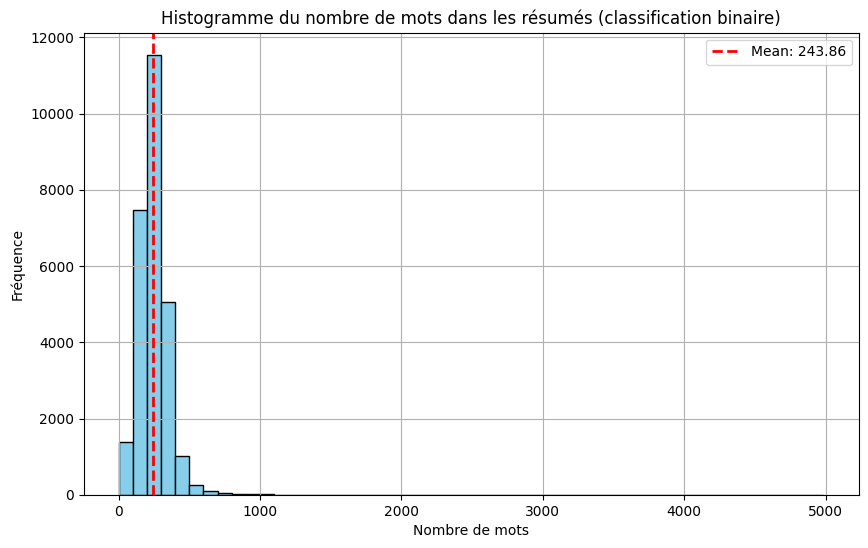
\includegraphics[width=0.5\linewidth]{word_distribution_per_abstract_binary_class.png}
\caption{Répartition du nombre de mots dans les résumés pour la tâche de classification binaire.}
\label{fig:word_distribution_binary_class}
\end{figure}

\begin{figure}[H]
\centering
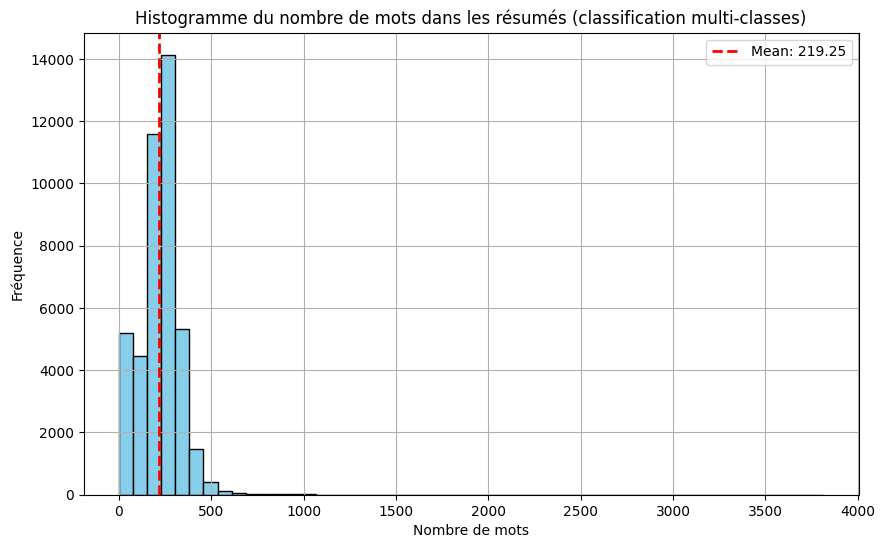
\includegraphics[width=0.5\linewidth]{word_distribution_per_abstract_multi_class.png}
\caption{Répartition du nombre de mots dans les résumés pour la tâche de classification multiclasses.}
\label{fig:word_distribution_multi_class}
\end{figure}

\begin{figure}[H]
\centering
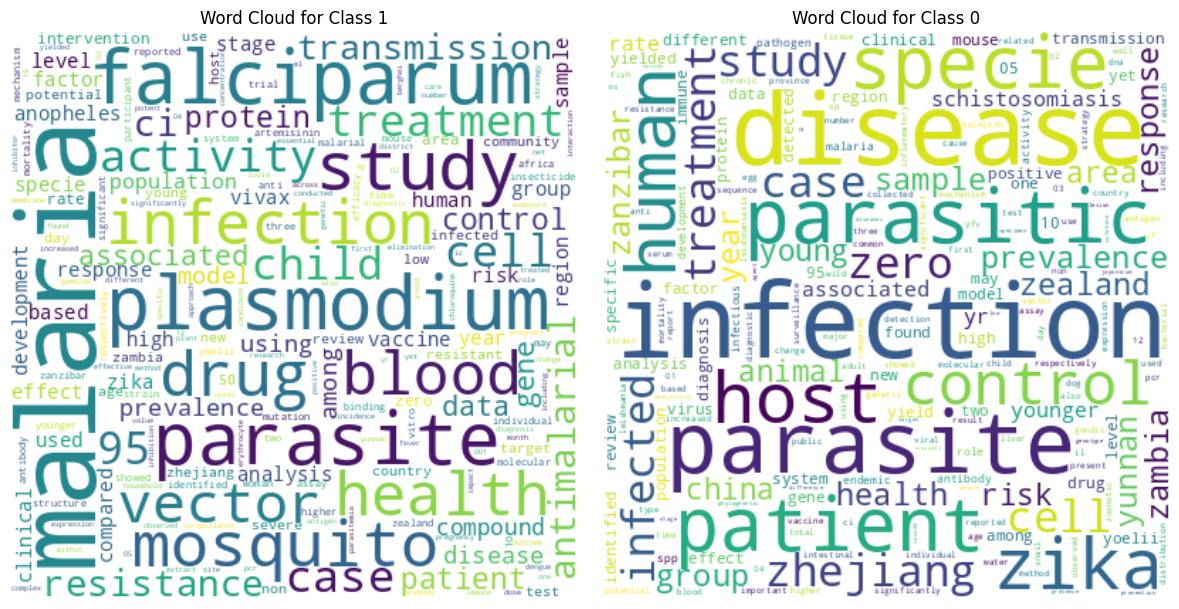
\includegraphics[width=0.75\textwidth]{binary_word_cloud.png}
\caption{Nuage de mots pour la classification binaire, illustrant les termes les plus fréquents associés à chaque classe.}
\label{fig:binary_word_cloud}
\end{figure}

\begin{figure}[H]
\centering
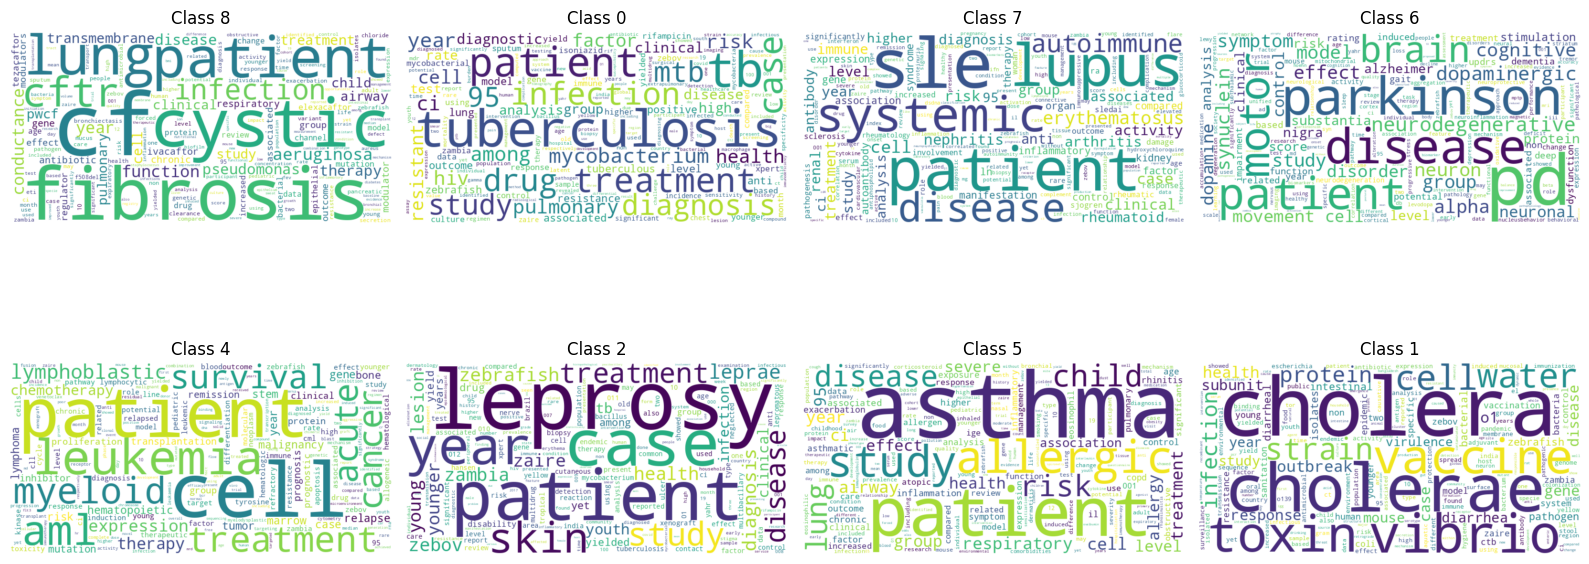
\includegraphics[width=0.9\textwidth]{multi_word_cloud.png}
\caption{Nuage de mots pour la classification multiclasses, illustrant les termes dominants pour chaque catégorie de maladie(pour 8 classes).}
\label{fig:multi_word_cloud}
\end{figure}

\begin{figure}[H]
\centering
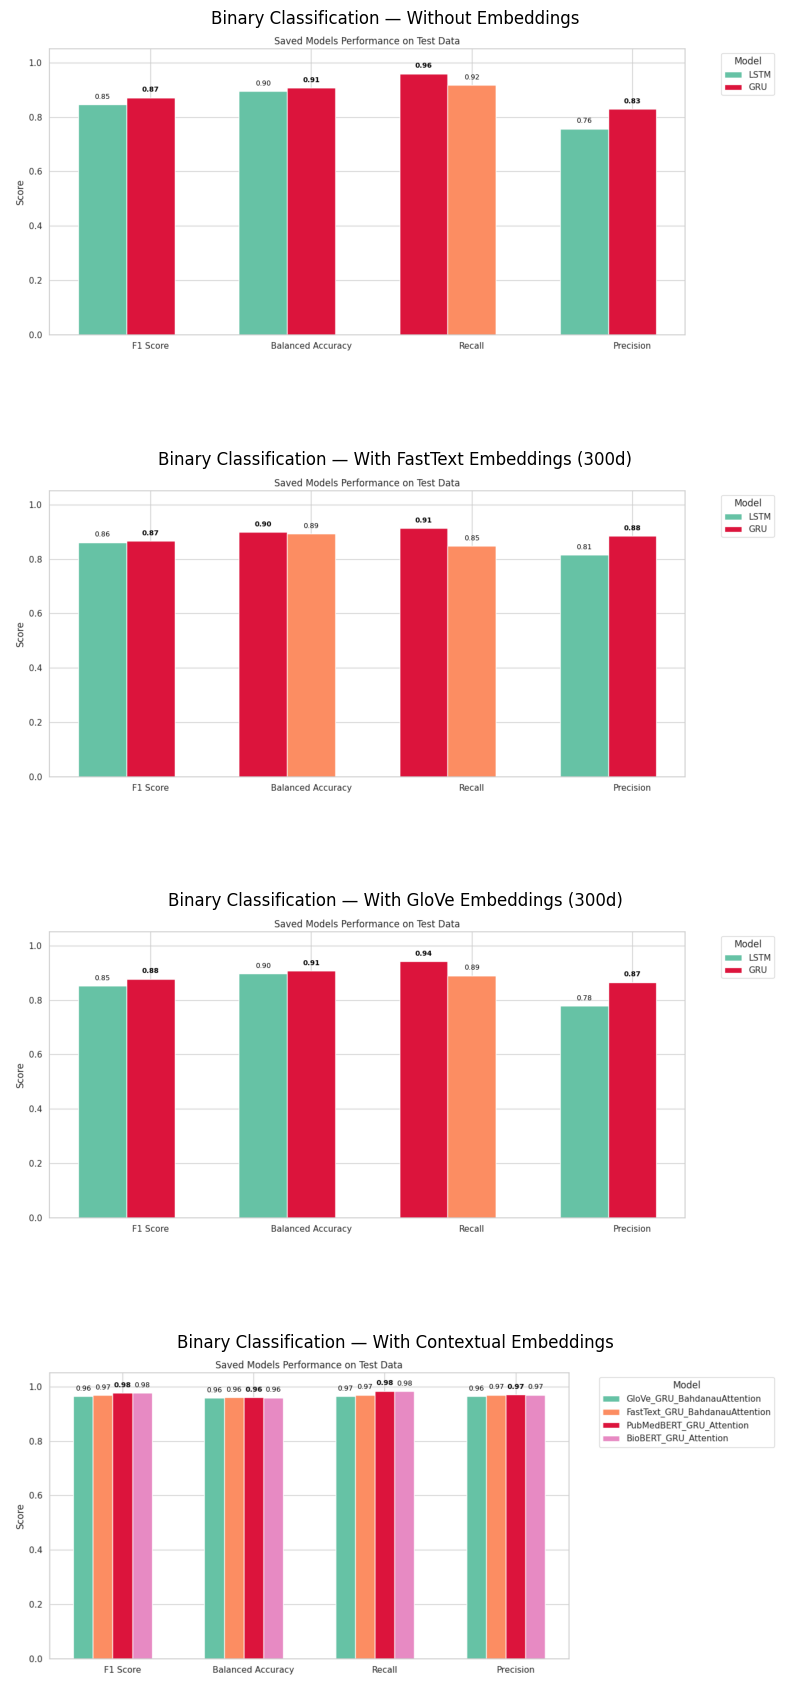
\includegraphics[width=0.6\textwidth]{model_performances_binary.png}
\caption{Performances des modèles (classification binaire)}
\label{fig:model_performances_binary}
\end{figure}

\begin{figure}[H]
\centering
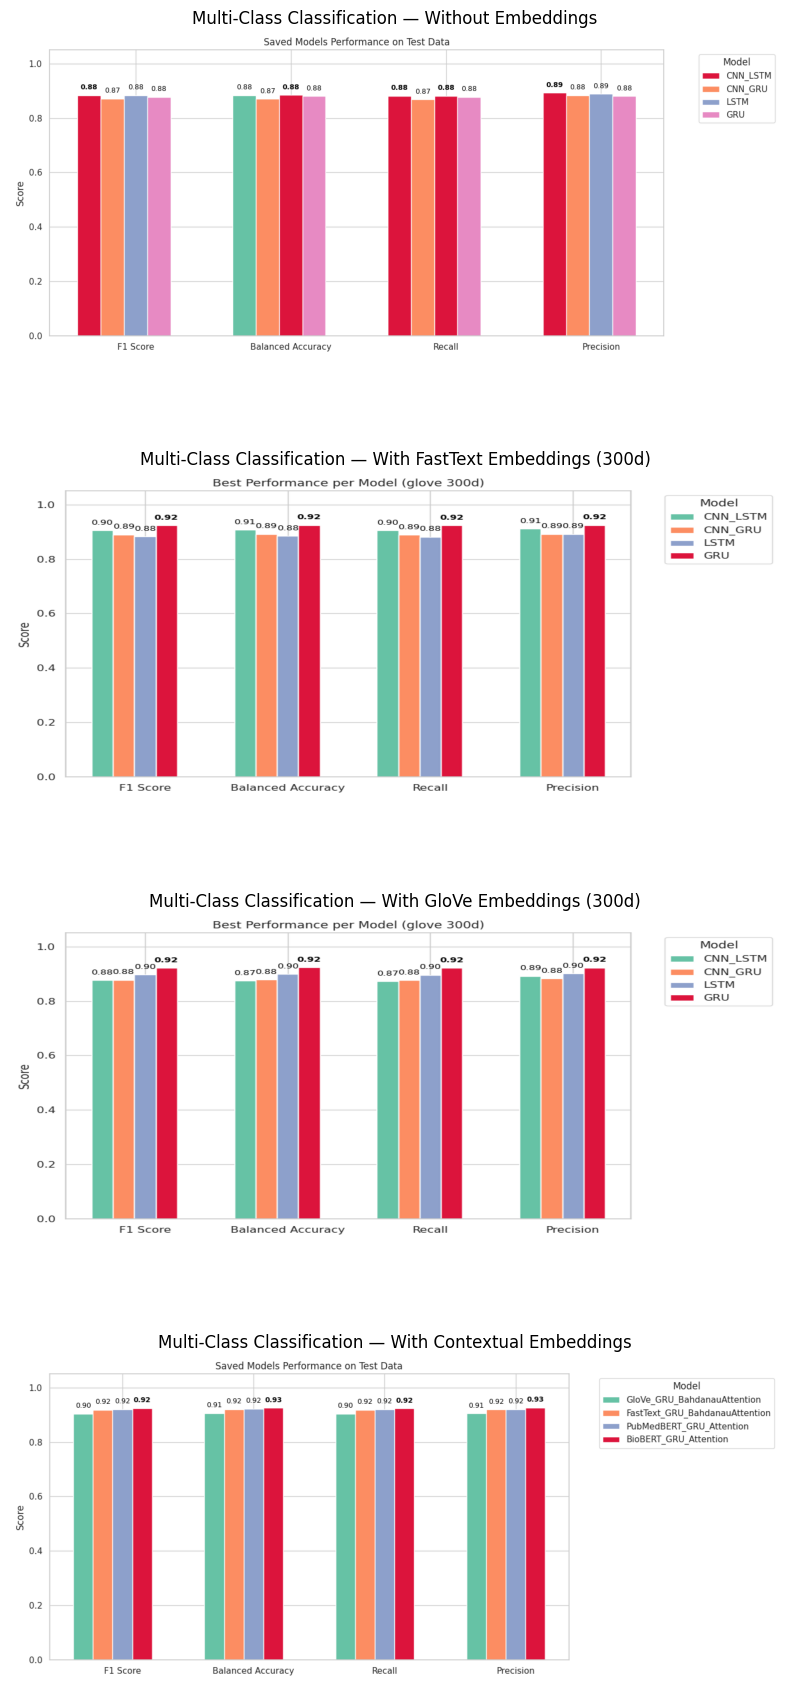
\includegraphics[width=0.6\textwidth]{multi_class_performances.png}
\caption{Performances des modèles (classification multiclasses)}
\label{fig:multi_class_performance}
\end{figure}

\begin{figure}[H]
\centering
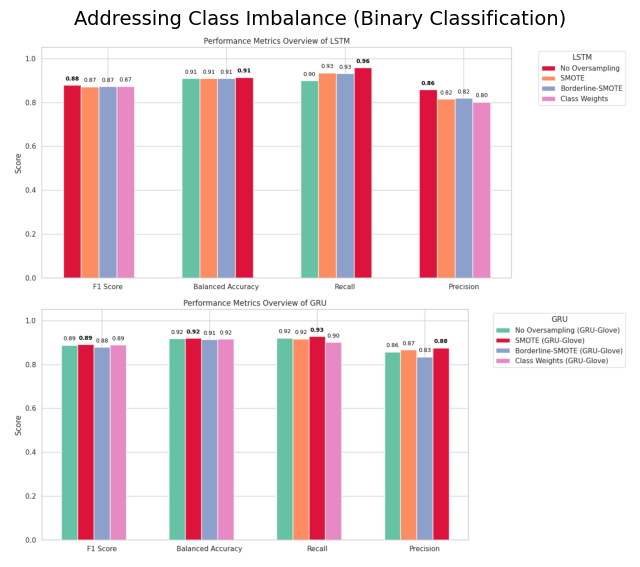
\includegraphics[width=0.6\textwidth]{resampling.png}
\caption{Performances des modèles GRU et LSTM après application des techniques de rééchantillonnage (SMOTE, Borderline-SMOTE) et de pondération des classes dans la fonction de perte (classification binaire).}
\label{fig:resampling}
\end{figure}

\begin{figure}[H]
\centering
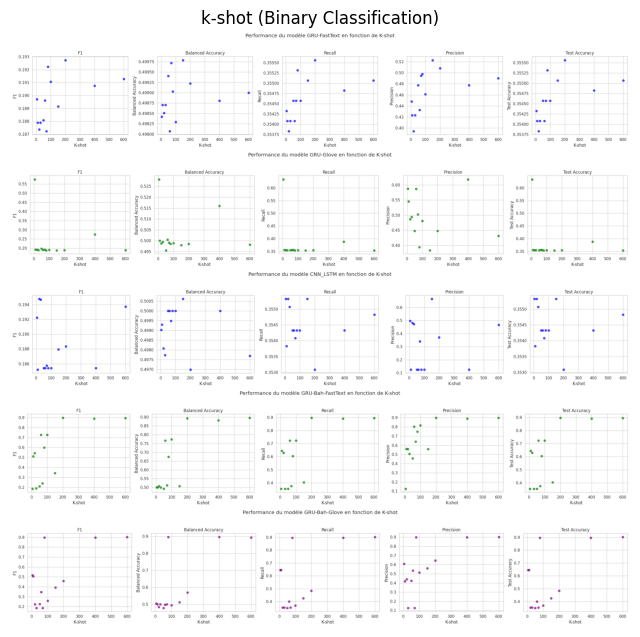
\includegraphics[width=0.7\textwidth]{kshot_binary.png}
\caption{k-shot (Binary Classification)}
\label{fig:kshot_binary}
\end{figure}

\begin{figure}[H]
\centering
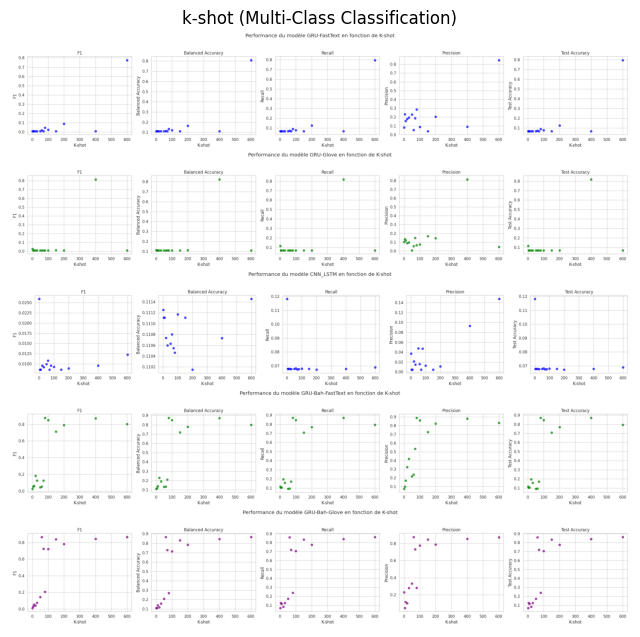
\includegraphics[width=0.7\textwidth]{kshot_multi.png}
\caption{k-shot (Multi-Class Classification)}
\label{fig:kshot_multi}
\end{figure}

\begin{figure}[H]
\centering
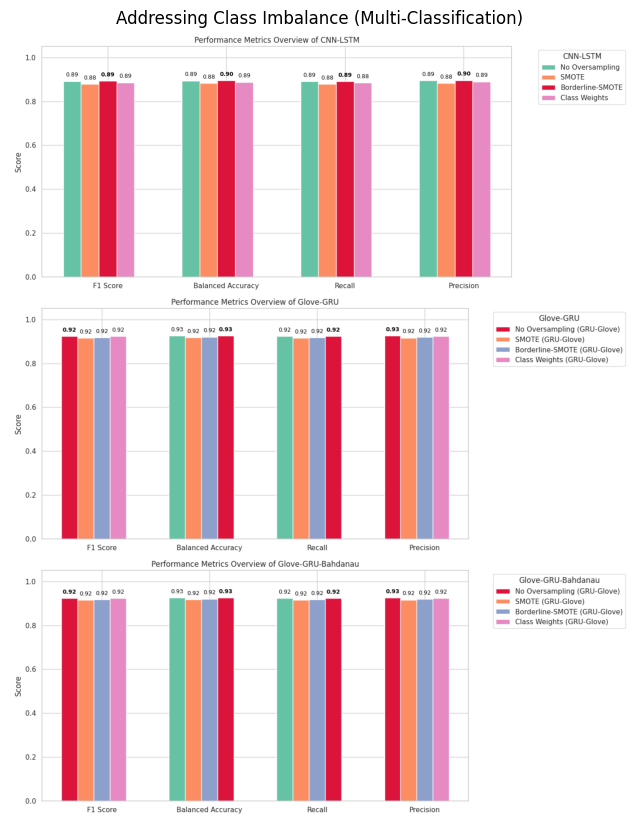
\includegraphics[width=0.5\textwidth]{resampling_multi.png}
\caption{Performances des modèles GRU et LSTM après application des techniques de rééchantillonnage (SMOTE, Borderline-SMOTE) et de pondération des classes dans la fonction de perte (Classification Multiclasses).}
\label{fig:resampling_multi}
\end{figure}


\begin{figure}[H]
\centering
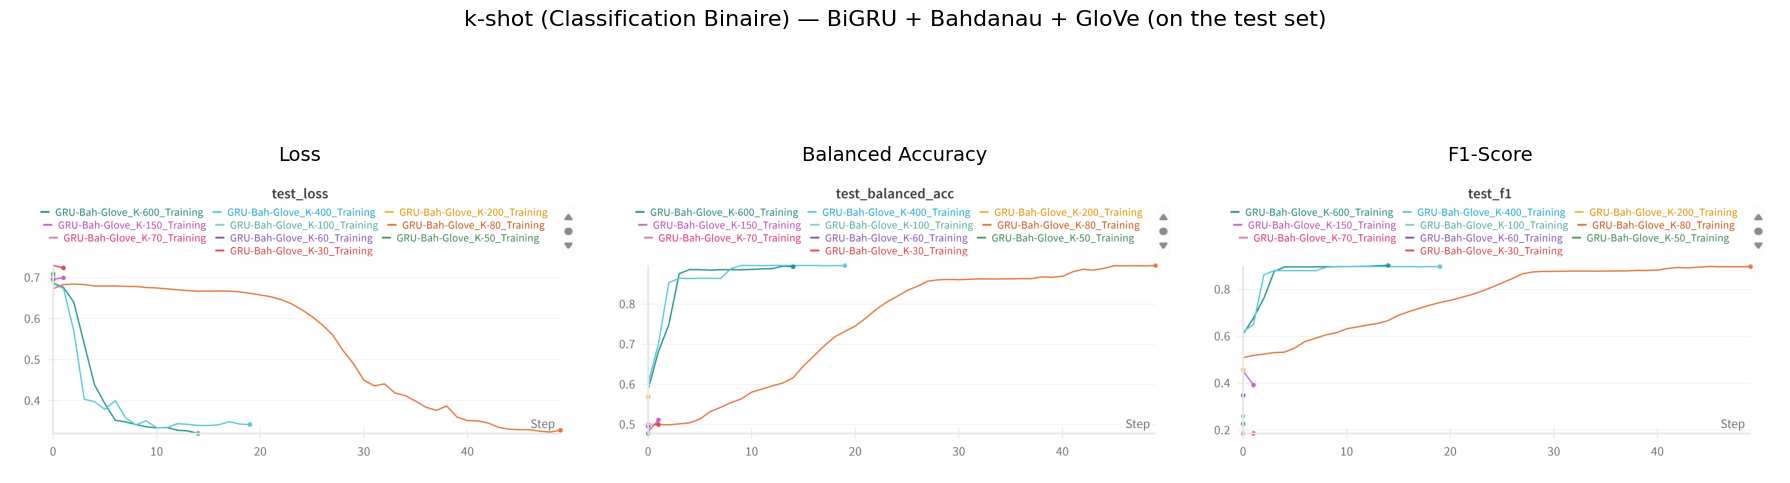
\includegraphics[width=1\textwidth]{kshot_binary_biGRU.png}
\caption{Évolution de la perte, du F1-score et de la Balanced Accuracy pour le modèle BiGRU + Bahdanau + GloVe selon la valeur de $k$ (classification binaire).}
\label{fig:kshot_binary_bi_Gru}
\end{figure}

\begin{center}
\begin{minipage}[t]{\textwidth}
\centering
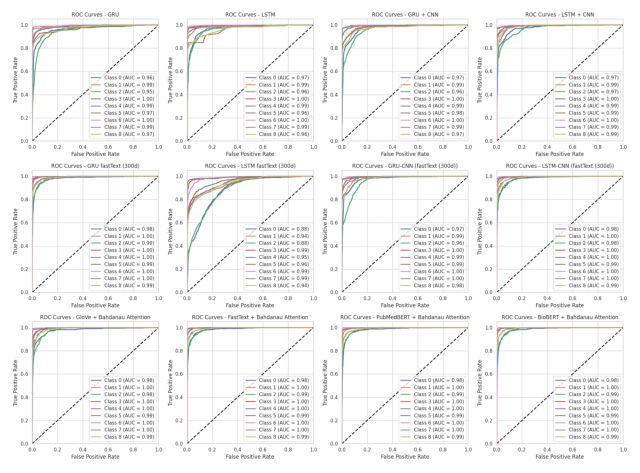
\includegraphics[width=\linewidth]{auc_multi_class.png}
\small\textbf{Figure:} AUC Curve for Multi-Class Classification
\label{fig:auc_multi}
\end{minipage}
\end{center}
\begin{figure}[H]
\centering
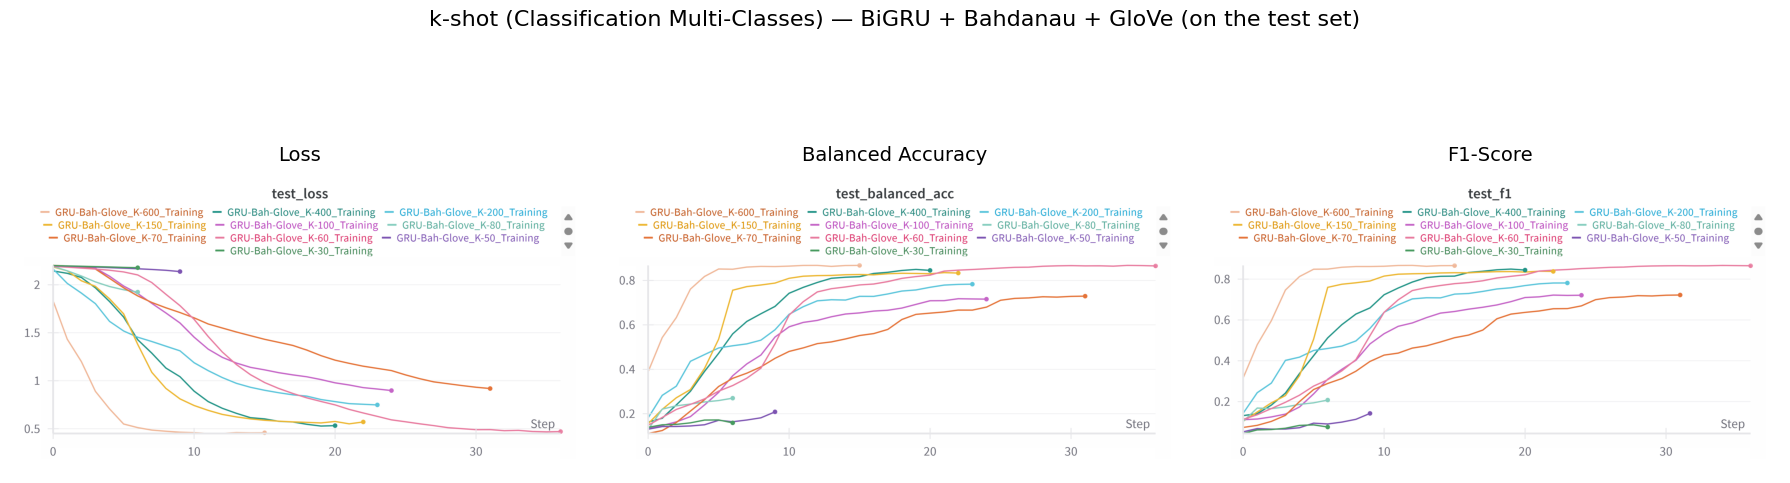
\includegraphics[width=1\textwidth]{kshot_multi_biGRU.png}
\caption{Évolution de la perte, du F1-score et de la Balanced Accuracy pour le modèle BiGRU + Bahdanau + GloVe selon la valeur de $k$ (classification multiclasses).}
\label{fig:kshot_multi_bi_Gru}
\end{figure}

\begin{figure}[H]
\centering
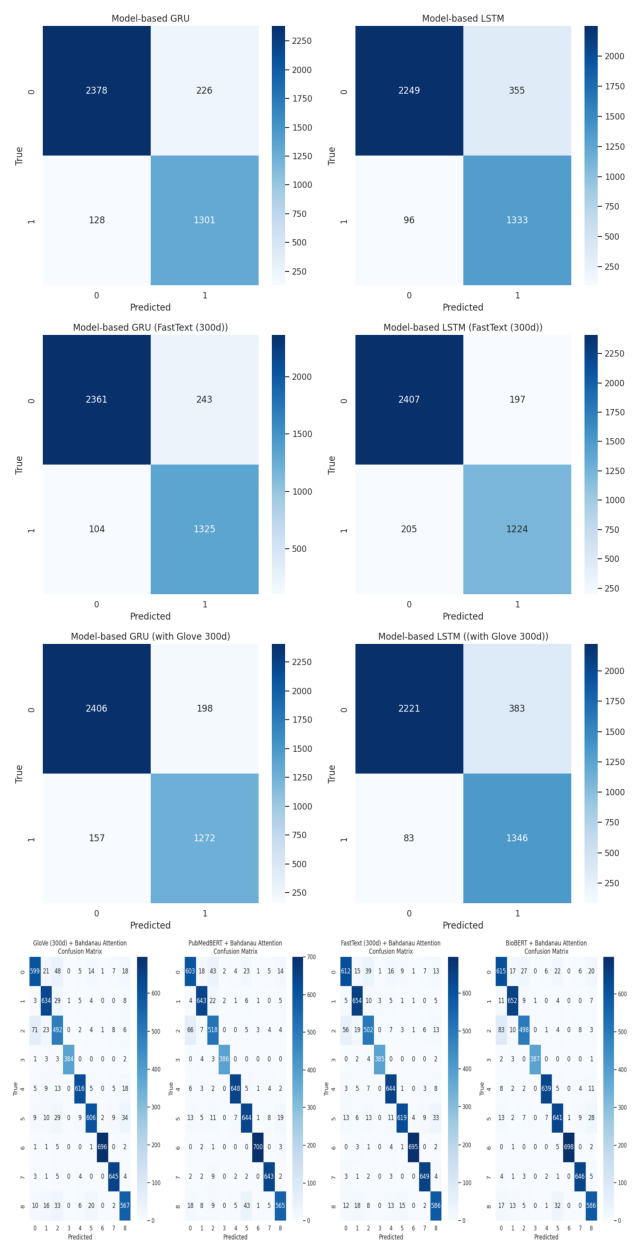
\includegraphics[width=0.8\linewidth]{cm_binary.png}
\caption{Confusion matrices for Binary Classification}
\label{fig:cm_binary}
\end{figure}

\begin{figure}[H]
\centering
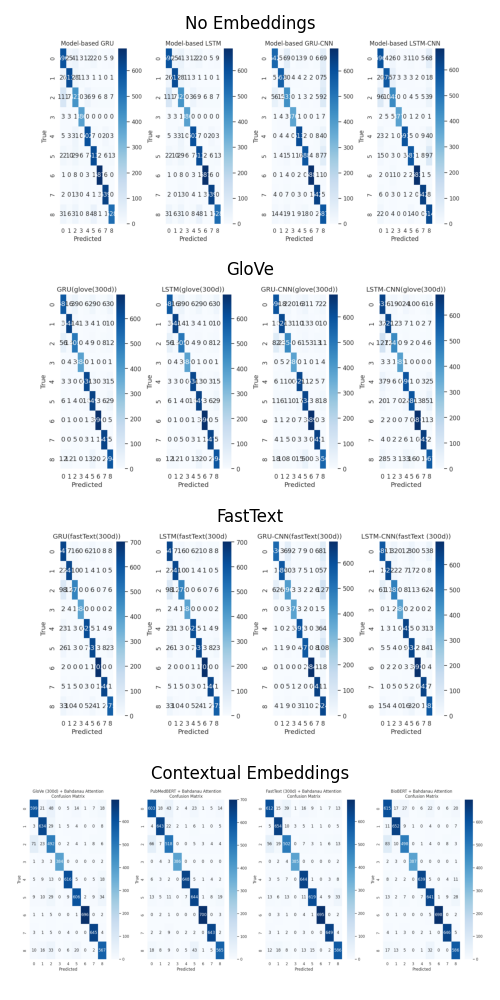
\includegraphics[width=0.8\linewidth]{cm_multi.png}
\caption{Confusion matrices for Multi-Class Classification}
\label{fig:cm_multi}
\end{figure}

\begin{figure}[H]
\centering
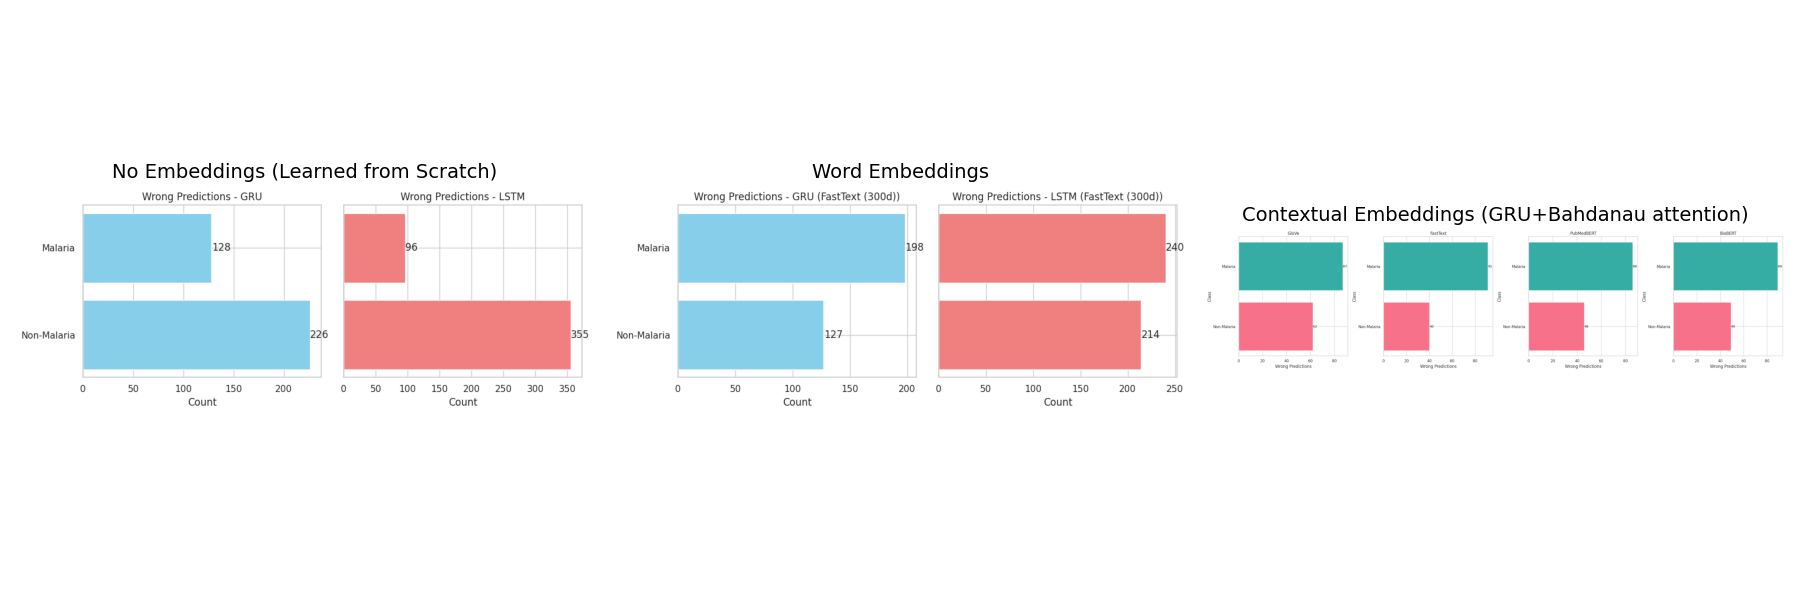
\includegraphics[width=0.8\linewidth]{binary_misclass_results.png}
\caption{Misclassifications for Binary Classification}
\label{fig:binary_misclass}
\end{figure}

\begin{figure}[H]
\centering
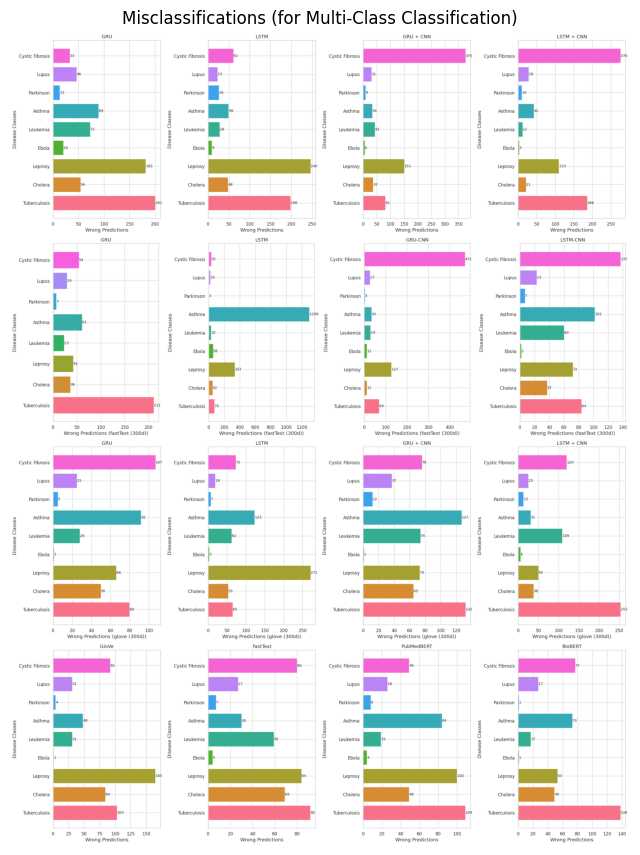
\includegraphics[width=0.8\linewidth]{multi_misclassifications.png}
\caption{Misclassifications for Multi-Class Classification}
\label{fig:multi_misclassifications}
\end{figure}


































\newpage
\begin{thebibliography}{99}

\bibitem{bahdanau2015neural}
D. Bahdanau, K. Cho, and Y. Bengio, 
\textit{Neural Machine Translation by Jointly Learning to Align and Translate}, 
International Conference on Learning Representations (ICLR), 2015. 
\url{https://arxiv.org/abs/1409.0473}

\bibitem{bengio1994learning}
Y. Bengio, et al., 
\textit{Learning long-term dependencies with gradient descent is difficult}, 
IEEE Transactions on Neural Networks, vol. 5, no. 2, pp. 157–166, 1994.

\bibitem{bojanowski2017enriching}
P. Bojanowski, E. Grave, A. Joulin, and T. Mikolov, 
\textit{Enriching word vectors with subword information}, 
Transactions of the Association for Computational Linguistics, vol. 5, pp. 135–146, 2017. 
\url{https://aclanthology.org/Q17-1010/}

\bibitem{brodersen2010balanced}
K. H. Brodersen, C. S. Ong, K. E. Stephan, and J. M. Buhmann, 
\textit{The balanced accuracy and its posterior distribution}, 
20th International Conference on Pattern Recognition, 2010.

\bibitem{cho2014learning}
K. Cho, B. van Merriënboer, D. Bahdanau, and Y. Bengio, 
\textit{Learning phrase representations using RNN encoder-decoder for statistical machine translation}, 
arXiv preprint arXiv:1406.1078, 2014. 
\url{https://arxiv.org/abs/1406.1078}

\bibitem{devlin2019bert}
J. Devlin, M. W. Chang, K. Lee, and K. Toutanova, 
\textit{BERT: Pre-training of deep bidirectional transformers for language understanding}, 
NAACL-HLT 2019, pp. 4171–4186, 2019. 
\url{https://arxiv.org/abs/1810.04805}

\bibitem{elman1990finding}
J. L. Elman, 
\textit{Finding structure in time}, 
Cognitive Science, vol. 14, no. 2, pp. 179–211, 1990.

\bibitem{finn2017model}
C. Finn, P. Abbeel, and S. Levine, 
\textit{Model-Agnostic Meta-Learning for Fast Adaptation of Deep Networks}, 
ICML 2017, pp. 1126–1135, 2017. 
\url{https://arxiv.org/abs/1703.03400}

\bibitem{gupta2021pubmedbert}
A. Gupta and A. Agarwal, 
\textit{PubMedBERT: A pre-trained biomedical language representation model for PubMed abstracts}, 
arXiv preprint arXiv:2102.09714, 2021. 
\url{https://arxiv.org/abs/2102.09714}

\bibitem{he2009learning}
H. He, X. L. Chen, and D. W. Song, 
\textit{Learning from imbalanced data}, 
Proceedings of the IEEE International Conference on Data Mining, 2009.

\bibitem{hochreiter1997long}
S. Hochreiter and J. Schmidhuber, 
\textit{Long short-term memory}, 
Neural Computation, vol. 9, no. 8, pp. 1735–1780, 1997.

\bibitem{lu2020pubmedbert}
Z. Lu et al., 
\textit{PubMedBERT: Pre-trained language model for biomedical text mining}, 
[Journal/Conference], 2020. 
\url{https://arxiv.org/abs/2007.XXX}

\bibitem{jia2019deep}
L. Jia, et al., 
\textit{Deep learning for medical text mining: A survey}, 
Journal of Biomedical Informatics, vol. 96, pp. 103–118, 2019.

\bibitem{jin2019recurrent}
Q. Jin, B. Dhingra, X. Liu, W. Cohen, and E. Hovy, 
\textit{Recurrent neural network models for disease name recognition using domain-invariant features}, 
In Proceedings of the BioNLP 2019 Workshop, pp. 1–10, 2019.

\bibitem{lee2020biobert}
J. Lee, W. Yoon, S. Kim, D. Kim, and C. H. So, 
\textit{BioBERT: A pre-trained biomedical language representation model for biomedical text mining}, 
Bioinformatics, vol. 36, no. 4, pp. 1234–1240, 2020. 
\url{https://doi.org/10.1093/bioinformatics/btz682}

\bibitem{mikolov2010recurrent}
T. Mikolov, M. Karafiát, L. Burget, J. Černocký, and S. Khudanpur, 
\textit{Recurrent neural network based language model}, 
In Interspeech, vol. 2, pp. 1045–1048, 2010.

\bibitem{mikolov2018advances}
T. Mikolov and others, 
\textit{Advances in pretraining models}, 
Journal of Machine Learning, vol. 10, pp. 1–10, 2018.

\bibitem{pennington2014glove}
J. Pennington, R. Socher, and C. D. Manning, 
\textit{GloVe: Global Vectors for Word Representation}, 
In Proceedings of the 2014 Conference on Empirical Methods in Natural Language Processing (EMNLP), pp. 1532–1543, 2014. 
\url{https://aclanthology.org/D14-1162/}

\bibitem{snell2017prototypical}
J. Snell, K. Swersky, and R. Zemel, 
\textit{Prototypical Networks for Few-shot Learning}, 
NeurIPS 2017, pp. 4077–4087, 2017. 
\url{https://arxiv.org/abs/1703.05175}

\bibitem{vinyals2016matching}
O. Vinyals, C. Blundell, T. Lillicrap, D. Wierstra, and D. Silver, 
\textit{Matching Networks for One-Shot Learning}, 
NeurIPS 2016, pp. 3630–3638, 2016. 
\url{https://arxiv.org/abs/1606.04080}

\bibitem{yin2017comparative}
W. Yin, K. Kann, M. Yu, and H. Schütze, 
\textit{Comparative study of CNN and RNN for natural language processing}, 
arXiv preprint arXiv:1702.01923, 2017. 
\url{https://arxiv.org/abs/1702.01923}

\bibitem{zhang2020biowordvec}
Y. Zhang, Q. Chen, Z. Yang, H. Lin, and Z. Lu, 
\textit{BioWordVec, improving biomedical word embeddings with subword information and MeSH}, 
Scientific Data, vol. 6, no. 52, 2020. 
\url{https://doi.org/10.1038/s41597-019-0055-0}

\bibitem{saito2015precision}
T. Saito and M. Rehmsmeier, 
\textit{The Precision-Recall Plot is More Informative than the ROC Plot When Evaluating Binary Classifiers on Imbalanced Datasets}, 
PLOS ONE, vol. 10, no. 3, 2015.

\bibitem{japkowicz2002class}
N. Japkowicz and S. Stephen, 
\textit{The class imbalance problem: A systematic study}, 
Intelligent Data Analysis, vol. 6, no. 5, pp. 429–449, 2002.

\bibitem{chawla2002smote}
Chawla, N.V., Bowyer, K.W., Hall, L.O., \& Kegelmeyer, W.P. (2002).
SMOTE: Synthetic Minority Over-sampling Technique.
\textit{Journal of Artificial Intelligence Research}, \textbf{16}, 321--357.

\bibitem{han2005borderline}
Han, H., Wang, W.Y., \& Mao, B.H. (2005).
Borderline-SMOTE: A New Over-Sampling Method in Imbalanced Data Sets Learning.
In \textit{Proceedings of the International Conference on Intelligent Computing}, Springer, 878--887.

\bibitem{Chawla2002SMOTE} Chawla, N. V., \textit{SMOTE: Synthetic Minority Over-sampling Technique}, Journal of Artificial Intelligence Research, 2002.

\bibitem{Han2005Borderline} Han, H., Wang, W. Y., and Mao, B. H., \textit{Borderline-SMOTE: A New Over-Sampling Method in Imbalanced Data Sets Learning}, Proceedings of the International Conference on Intelligent Computing, 2005.

\bibitem{King2001Logit}
G. King and L. Zeng, 
\textit{Logistic Regression in Rare Events Data}, 
Political Analysis, vol. 9, no. 2, pp. 137–163, 2001.

\bibitem{Lin2017Focal}
T.-Y. Lin, P. Goyal, R. Girshick, K. He, and P. Dollár,
\textit{Focal Loss for Dense Object Detection}, 
Proceedings of the IEEE International Conference on Computer Vision (ICCV), pp. 2980–2988, 2017.

\bibitem{van2008visualizing}
L.J.P. van der Maaten and G.E. Hinton,
\textit{Visualizing data using t-SNE},
Journal of Machine Learning Research, vol. 9, pp. 2579–2605, 2008.

\bibitem{zhou2015text}
P. Zhou, Z. Qi, S. Zheng, J. Xu, H. Bao, and B. Xu, 
\textit{Text Classification Improved by Integrating Bidirectional LSTM with Two-dimensional Max Pooling}, 
Proceedings of the 26th International Conference on Computational Linguistics (COLING), 2016, pp. 3485–3495. 
\url{https://aclanthology.org/C16-1329}

\bibitem{kim2014convolutional}
Y. Kim,
"Convolutional Neural Networks for Sentence Classification,"
Proceedings of the 2014 Conference on Empirical Methods in Natural Language Processing (EMNLP), 2014.
\url{https://arxiv.org/abs/1408.5882}

\bibitem{zhou2015clstm}
C. Zhou, C. Sun, Z. Liu, and F. Lau,
"A C-LSTM Neural Network for Text Classification,"
arXiv preprint, 2015.
\url{https://arxiv.org/abs/1511.08630}

\bibitem{gu2020domain}
Y. Gu, R. Tinn, H. Cheng, M. Lucas, N. Usuyama, X. Liu, T. Naumann, J. Gao, H. Poon, "Domain-specific language model pretraining for biomedical natural language processing," ACM Transactions on Computing for Healthcare (HEALTH), vol. 3, no. 1, pp. 1–23, 2020. \url{https://arxiv.org/abs/2007.15779}

\bibitem{geurts2006} 
Geurts, P., \& Wehenkel, L. (2006). \textit{Learning with Decision Trees and Random Forests}. Institut Montefiore, University of Liège, Belgium.





























\end{thebibliography}
\end{document}
-------------------------------------------------------------------------------------------------------------------------------




